\documentclass[a4paper,11pt]{article}
\usepackage[utf8]{inputenc}
\usepackage{dmasproject}
% if you need additional LaTeX packages, add them here
\usepackage[T1]{fontenc}
\usepackage{newpxtext,newpxmath}
% \usepackage[left=1in, right=1in, top=1.25in, bottom=1.25in]{geometry}
\usepackage{hyperref}
\usepackage{titling}

% \usepackage{caption}
\usepackage{amsmath}
\usepackage{mathtools}
\usepackage{amsfonts}
\usepackage{amssymb}
\label{mathrefs}

\usepackage{graphicx}
\usepackage{multirow}
\usepackage{pdflscape}

% Remove paragraph indent and add space between paragraphs
\usepackage{parskip}
\setlength{\parindent}{0pt}

\begin{document}

% Ask zain and connor to review safety/regulatory section and update
% Waleed help with proj management (sec 9)

%% BEGIN TITLE
\begin{titlingpage}
    \begin{center}
        {\huge\bfseries%
            University of Waterloo \\
        }
        \vspace{1em}
        {\Large\bfseries%
            Faculty of Engineering \\
            \vspace{1em}
            GENE 403 Design Project Report \\
        }
        
        \vspace{15em}
    
        % Heading
        {\Huge\bfseries%
            Glasses for the Visually Impaired \\[0.5em]
        }

        \vspace{15em}
        
        % Authors
        Prepared by: \\
        \vspace{1em}
        \begin{tabular}{cccc}
            Martin Ethier \\
            MME \\
            20660931 \\
            methier
        \end{tabular}
        
        \vspace{9em}
        
        December 8th, 2021
        
    \end{center}
\end{titlingpage}
%% END TITLE

\newpage

\tableofcontents

\newpage

\section{Comparison to Spring 2021 Report}

This report is meant to outline the work that was done by Martin during the Fall 2021 term. However, the required content for some of the sections has remained the same since then. Instead of referring to the Spring 2021 report, the content was copied into this report, in order to have all the necessary information in one report. The following sections are the sections which were mostly taken from the Spring 2021 report, indicated by section number: 2, 3, 6, 7, 8, 9, 15.1, 15.3, 15.4, 15.6

\section{Introduction}
The latest global estimates found that about 253 million people are visually impaired. Of those people, about 36 million are blind, meaning they have little to no vision \cite{orbis-global-blind-data}. Looking specifically at Canada and the United States, an estimated 1.5 million Canadians identify themselves as having sight loss \cite{cnib-blind-data}, and about 7.6 million Americans have a visual disability \cite{nfb-blind-data}. The Vision Loss Expert Group predicts that without increased access to eye health services, these numbers could potentially triple by 2050 \cite{orbis-global-blind-data}.

Taking a step back, it is worth investigating what being visually impaired or blind actually means. In one of our focus interviews, we were told by somebody who self-identified as blind that "Blindness is a spectrum". Very few people who identify as visually impaired or blind have no light perception at all. For most, blindness is a gradual degradation of sight. Some can see well, but only in certain light conditions. Others can only identify shapes or colours, and some have a field of vision so diverse and complex that is difficult to explain \cite{lighthouse-sf-info-page}. Another diverse aspect of blindness is when it is experienced in life. Some individuals are blind from birth, while others develop it at various points in life. While there are many causes of blindness, the leading ones are cataracts, age-related macular degeneration, glaucoma, diabetic retinopathy, corneal opacity, and trachoma \cite{WHO-blindness}.

Despite the diversity of conditions and visual impairment out there, there are many common problems faced by this demographic. One of the biggest ones, and a core focus of our project, is reading text. It doesn't occur to sighted individuals just how much text there is out in the world that contains crucial information we rely on to go about our day. Many visually impaired folk do not have this luxury and are missing out on key information that can help them to live more independently. While one solution to this is to ensure accompanying braille text wherever possible, there are still many situations where braille is not available. For example, text on a storefront or a postcard with your name and address on it to let you know the mail is for you.

Our design solution is to take advantage of cutting-edge advancements in artificial intelligence and computer vision to extract, decode, and communicate information from an image to a visually impaired user through audio transcription. More specifically, we are designing a mobile application and a wearable device (glasses) that will enable the ability to conveniently and efficiently accomplish this task. Some design solutions already exist to accomplish our proposed primary function, and they are described in the need analysis summary (Section \ref{need-analysis-summary}).

This report summarizes the need analysis, research, verification, development, and project management carried out in the Fall 2021 term as a part of GENE 403 for our initial low fidelity prototype. Note that this report mostly is made to highlight the work that was done by Martin Ethier over the Fall 2021 term. Martin worked on the computer vision algorithms that process the images taken with the device. The other members of the group also made significant progress, and summaries of their work will be made in the report, but it is not the main focus.

\newpage
\subsection{Key Terminology}

\setlength{\tabcolsep}{1em}
\begin{table}[ht]
    \centering
    \begin{tabular}{|p{5cm}|p{10cm}|}
        \hline
        Optical Character Recognition (OCR) & Broad term that describes any system that can extract and decode text from a digital representation such as an image or PDF \\ \hline
        iOS & Operating system used in Apple iPhones \\ \hline
        VoiceOver & Screen reader built into iOS \\ \hline
        Text-to-speech & Program that takes in text data and converts it to speech data \\ \hline
        MFi Chip & Specialty chip needed for certain wireless capabilities when communicating with Apple devices \\ \hline
        System on a chip (SoC) & Integrated circuit that integrates the components of a computer \\ \hline
        Raspberry PI Zero W & Very small single-board computer with wireless capabilities \\ \hline
    \end{tabular}
\end{table}

\section{Need Analysis Summary}
Note that this needs analysis was done during the Spring 2021 term. Since we were satisfied with the results from this analysis, no further analysis was done for the Fall 2021 term. For context in this report, the needs analysis summary from Spring 2021's report is included.

\label{need-analysis-summary}

\subsection{Problem Identification}
Since none of the group members are visually impaired, it was important to us to perform need analysis through speaking with individuals who are visually impaired or organizations that represent them. Doing this provided us with useful insight into some of the problems faced by the visually impaired, and allowed us to zero in on the features that would be the most useful to include in our design solution. Through our own research along with recommendations from our faculty advisor, Professor John Zelek, we identified a few organizations that advocate and aid the visually impaired that would be insightful to connect with. We were fortunate enough to hear back and have a chance to speak with a representative from Lighthouse SF and the University of Waterloo's AccessAbility Services.

\subsubsection{Interview with Lighthouse SF}
Lighthouse SF is an organization founded in 1902 and currently has headquarters in San Francisco, California. Their goal is to promote the independence, equality, and self-reliance of people who are blind or have low vision \cite{lighthouse-sf-homepage}. They pool together resources, hold seminars, and offer courses to help people with visual disabilities learn to use the latest and greatest assistive technologies. The individual that we had a chat with is currently an assistive technology instructor at the organization and self-identified herself as being blind.

During the interview, we discussed the various assistive technologies that exist and what her experience was with using them. She also enumerated a few very specific use cases where OCR technology currently does well, and where there is room for improvement. Some key takeaways were:

\begin{itemize}
    \item In the context of reading a physical book, one useful feature would be if the technology can automatically detect when the page has been turned and start reading out the next page without any additional explicit input from the user.
    \item There are two widely used "visual interpreter" apps called Be My Eyes and Aira. These apps connect the user with a sighted individual through a video call to assist in a task. The key difference between the two apps is that Be My Eyes works through sighted volunteers who lend their time for free and do not require any professional training, while Aira employs agents that are professionally trained visual interpreters to respond to calls.
    \item In the context of OCR, she mentioned that the most useful feature amongst other apps was the ability to instantly read out the text from a video feed, and in the cases where an image needs to be captured, audio-guided camera capture was useful. An example of audio-guided capture is when you are trying to get a picture of a document, all 4 corners of the document need to be visible for the image processing pipeline to extract out just the document from the image. One app, in particular, will say things like "left corner not visible" to inform the user why the captured image was not sufficient.
    \item One of the complaints about current OCR technology is that it does not perform well on handwritten text or non-standard machine fonts.
    \item She gave us a great quote: "Blindness is a spectrum" when we asked about the usability of wearable glasses. She mentioned that due to the diversity amongst visually impaired folks, some might know how to put on and use glasses due to losing their sight later in life, but it might not be as intuitive to someone who has been blind since birth.
    \item Another feature we asked her about is above the waist obstacle detection using computer vision. She mentioned that this is a feature that is not present in many solutions, but warned us that it is not as useful of a feature as we might think. It is only applicable in few scenarios, many individuals already use a white cane that is cheap and very capable for obstacle detection/avoidance in most scenarios.
    \item She informed us of a monthly meetup called Lighthouse Labs where engineers and developers working on assistive technology for low vision come to present their ideas. She extended an invite for us to attend and showcase what we end up building.
\end{itemize}

Overall, our biggest takeaway from the interview with Lighthouse SF was to double down on OCR as the primary feature of our design, as we spent the most time talking about it and we got the impression that it is the feature that is most useful. While we do have other additional features in mind, such as depth estimation, scene description, and money detection, we don't plan on spending any time on those until we feel confident our OCR works well.

\subsubsection{Interview with UW AccessAbility Services}
AccessAbility Services is responsible for working with students with disabilities to develop personalized academic accommodations at the University of Waterloo \cite{uw-accessability}. We spoke with a representative from the office who was employed as an adaptive educational technologist. There are 3 functional areas the office focuses on: class, assignments, and tests. Examples of potential services provided within the context of a visually impaired student for each of the functional areas are:
\begin{itemize}
    \item Class
    \begin{itemize}
        \item Reserved seating in a classroom if a student wishes to sit closer to the front or back
        \item Request professors to provide a transcript of lecture slides
        \item Request professor to allow student to audio or video record the lectures so that they can listen and transcribe them later on their own
        \item Note-taking services, such as asking for student volunteers to provide notes
        \item Get a textbook translated into braille or audio format
    \end{itemize}
    
    \item Assignments
    \begin{itemize}
        \item Asking for extensions to accommodate for additional difficulties of learning the content with a disability
    \end{itemize}
    
    \item Tests
    \begin{itemize}
        \item Getting students a scribe
        \item Requesting for oral tests instead of written tests
        \item Exams are done in special test centres where computers are setup that can read out the text for each question
        \item Get a test translated into braille
    \end{itemize}
\end{itemize}

In addition, a few technologies/products were mentioned that students had used in the past, including:
\begin{itemize}
    \item Jaws: Screen reading technology for the Windows operating system \cite{jaws-software}
    \item Kurzweil 3000: Educational software with text to speech features \cite{kurzweil}, not specifically tailored for visually impaired users though
    \item Read\&Write by TextHelp: A literary support tool that has useful OCR features in it \cite{read-and-write}. However, similar to Kurzweil, it's targeted at a general audience, in particular, grade school students
    \item Speechify: Mobile and desktop app for those with reading difficulties, low vision, and anybody interested in converting reading material to an audio format. Can read anything from the web, PDF, or images \cite{speechify}
\end{itemize}

There are even more assistive technologies available, and a more comprehensive list along with tutorials on how to use them are available on learn by self-registering for AccessAbility Services, which is available for every student, regardless of whether or not they are registered with a disability.

When asked what some of the complaints students had about existing technologies, we were told that screen reading technology often gets thrown off by weird formatting (captions, footnotes, etc.), and sometimes the voice reading it out can be a bit robotic. Speechify was highlighted as having realistic voices that are more pleasant and engaging to listen to.

Our key takeaway from this interview was an overview of some of the difficulties faced by visually impaired students in the context of academics. We were also pointed towards a lot of currently available products and technologies that are adjacent to our proposed design solution. Additionally, we mentioned if it would be possible for us to send out a survey or request to speak with visually impaired students to provide us with informal discussion/feedback on our design solution. We were told this is something that could be organized if we wish to proceed, and we plan on exploring this avenue later on in our design process in order to conduct some user studies and testing on our design.

\subsection{Survey of Available Products/Technologies}
Many products and solutions already exist in our chosen problem space. Reviewing them closely and identifying the pros and cons of each one allowed us to focus on the things that could be done better and potentially addressed by our solution. The five products we choose to focus on are Orcam MyEye 2, Envision, Seeing AI, Speechify, and Be My Eyes. Others exist, but these five are the closest and most relevant to our proposed design solution, so they are most valuable to examine.

\subsubsection{OrCam MyEye 2}
The OrCam MyEye 2 \cite{orcam} is a piece of hardware that can be attached magnetically to an existing pair of glasses. It is designed specifically for blind and visually impaired users and has a wide array of features to support that demographic. It can be controlled by voice or touch and can accomplish tasks such as read text, recognize faces, identify products, recognize barcodes, recognize money, and identify colours. Best of all, it can do all these features offline, meaning a network connection is not required. This means all of the processing is done right on the glasses. When we first identified the problem space and thought of potential solutions, something like the OrCam MyEye 2 is precisely what we originally had in mind. However, what we quickly realized with this product and others like it is that they are very expensive. Pricing information isn't readily available without consultation with OrCam, but we did find an article \cite{orcam-price} that mentioned \$3500 USD. Additionally, OrCam listed it on Amazon for \$5800 CAD \cite{orcam-amazon}. Even though the exact pricing isn't clear, it seems that the cost for this device is multiple thousands of dollars, which is very high. Globally, there are an estimated 200 million people who do not have access to assistive products for low vision \cite{WHO-assistive}. One of the reasons for this is products can be very expensive, and some individuals with a visual impairment may not have sufficient financial resources to purchase products with a premium price tag.

While the technology in this product is cutting edge and very useful, we feel that with some design changes, primarily offloading compute to a server or a user's phone, it should be possible to deliver a similar feature set at a much more accessible price point. After examining the OrCam MyEye, we identified cost as our primary constraint and focused on finding a solution that can minimize it.

\subsubsection{Envision}
Envision has two products, an app and a pair of glasses, targeted for the visually impaired \cite{envision}. The app can be used on its own without the glasses, and it uses the phone's camera instead of a camera attached to glasses. The app has features for reading text, scene description, colour detection, barcodes, and configurable object and people detection. The app initially comes with a one-week free trial, and then afterward runs on a subscription model. As of August 7th, 2021, the prices in CAD for the app are below:
\begin{center}
    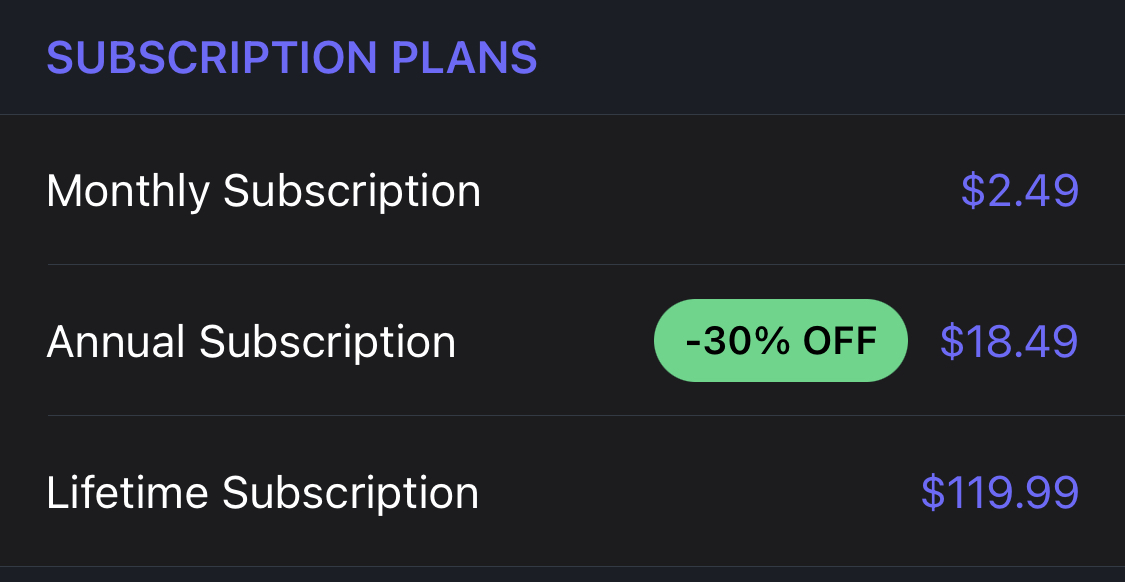
\includegraphics[width={0.7\linewidth}]{img/envision_app_price.jpeg}
\end{center}

Envision also has a pair of wearable glasses, built on top of the Google Glasses platform. All the features on the app are accessible with the glasses as well, as well as one additional feature that enables a video call that broadcasts a direct feed from the glasses. It is not clear from their website which of these features can run offline and which ones run online, as the glasses are capable of both wifi and Bluetooth. It's obvious that the video calling feature would require a network connection, but text detection could be done both offline or online. Additionally, the purchase of the glasses comes with a lifetime subscription to the accompanying application for both iOS and Android.

Similar to the OrCam MyEye, Envision is a great product with some cutting-edge features that are undeniably very useful for the visually impaired demographic. However, it suffers a similar problem in that it is very expensive. As of August 8th, 2021, the base model for Envision is listed as 3268.91 pounds, which is 5696.87 CAD.

\subsubsection{Seeing AI}
Seeing AI is a free application on iOS built as a part of Microsoft's "AI for Good" initiative \cite{seeing-ai}. Seeing AI has a lot of the same features that OrCam MyEye and Envision have, such as real-time short text detection, document reading, barcodes, face recognition, scene description, currency detection, and color detection. Two features that Seeing AI has that we couldn't confirm if MyEye or Envision have is handwritten text detection and light detection. Light detection is a unique feature that plays a sound that indicates how much light the camera detects. 

Some of these features work offline using on-device processing, while others utilize Microsoft's Azure cloud services and require a network connection. The features that require a network connection are document scanning, face detection, scene description, and handwritten text. The rest work offline.

The amazing part about this application is that it is totally free. There is no subscription or additional features available at a price. We found various other applications on the app store that would do a subset of features offered by Seeing AI, but they were not free. As a result, Seeing AI is considered the gold standard application for the visually impaired, as it is totally free and has a rich feature set. The individual we spoke to from Lighthouse SF was very familiar with this app and reported using it regularly.

After trying out this application, we really started to question if making a pair of glasses is even the way to go. If the end goal is to make it as cheap and accessible as possible, it's hard to compete with a free app that can do so much. The key insight that made us realize an affordable pair of glasses is still worthwhile to develop is the fact that it can be used without having to pull out and unlock your phone. Let's consider a specific example of wanting to read the name on a postcard. With Seeing AI, you'd have to pull out your phone, unlock it, find and open the Seeing AI app, switch to the "instant text" mode, and then have it read out the text for you. This might not seem so bad, but this process can be cumbersome for somebody who is visually impaired. However, with our solution, it would only require you to look towards the text you are trying to read, press a button on the glasses, and then after a small wait, the text will be read to you. This is fewer steps and allows you to more quickly read text out in the world. With this insight, we decided to continue pursuing our proposed design solution, even knowing now that a free alternative does exist.

\subsubsection{Speechify}
Speechify is a desktop and mobile app that can turn various forms of text into audio \cite{speechify}. The app is built on the premise that listening to something is easier and faster than reading it. It is not specifically for any demographic, but it can be used by anyone who has reading difficulty due to things like ADHD, Dyslexia, or visual impairment. Many people who have no problem reading still use Speechify, as it can increase productivity to get through large pieces of text faster by listening to it at faster speeds. Speechify can read anything on the internet, files, or images. It comes with a free option but there are paid features available, such as different voices that sound less robotic. This app was brought to our attention by UW AccessAbility services, as one of the complaints of many OCR technologies is the voice sounds very robotic, and Speechify was praised for having options for more realistic voices.

\subsubsection{Be My Eyes}
Be My Eyes is a free app that allows blind and visually impaired people to connect with sighted volunteers through a video call \cite{be-my-eyes}. This allows a sighted individual to assist in a task that a visually impaired person is having trouble with. Signing up to be a volunteer is free, and Connor has been a volunteer on the app for some time and has picked up three calls in the past. Waleed signed up for the app early in the term but has yet to get a notification to pick up a call. We examined this app as a way to potentially have interactions with visually impaired people, and get some insight into the kind of tasks that they need assistance with. An example use case would be for navigating an outdoor park. A visually impaired user may be in search of a bench to sit at and is not sure where to go. They can place a call for assistance on the app and a sighted volunteer will pick up and through the mobile phone's camera, guide the user to a nearby bench to sit at.

A notable mention is another app called Aira, which is built on the same premise as Be My Eyes, but instead of connecting visually impaired users with sighted volunteers, Aira employs trained visual interpreters who pick up the call.

Internally, we had some discussion about enabling a video call through the camera on the glasses, similar to the Envision glasses. This is not a high priority for us at the moment, but due to the success and usefulness of services such as Be My Eyes and Aira, it is something we are open to investigating further if time permits.

\subsubsection{Summary and Key Takeaways}
Assistive devices for the visually impaired is a problem space that has existed for quite some time, and as such, many solutions and products are currently available. Products like the OrCam MyEye 2, Envision, and Seeing AI offer a rich feature set and try to cover as many use cases as possible. The common feature, and the first one that each solution talks about, is the ability to detect and read text using OCR technology. It is reasonable to conclude that this is the most useful feature present in these solutions, and likely the one that gets the most usage. Therefore, we are choosing to focus on OCR as our primary feature, and only once we have that down will we start to consider some of the other features.

Additionally, due to the existence of Seeing AI, we plan on focusing our user experience around the glasses as much as possible. While we do want our app to eventually work without the glasses as well, and the user can simply use their phone's camera, it is less important to us since this functionality is already covered and implemented very well by Seeing AI. Our goal is to push this problem space forward with something that isn't too similar with what already exists.

\subsection{Patent Surveys}
The breadth of existing products with the same functionality as our solution has required us to carefully consider patent law when planning the design of our project. Specifically, OrCam owns a variety of patents protecting both their hardware and software products \cite{orcam-patents}. As the MyEye 2 is the device that most closely resembles our solution, we used their patent list as a starting point for our research. Other products, such as EnVision and NuEyes, possess IP as well, although these patents are either pending \cite{envision-patent} or unrelated to our solution.

Conveniently, the reason OrCam products are so expensive is also the reason we can successfully avoid patent infringement in our design. OrCam's patents are entirely related to proprietary software \cite{orcam-software} and hardware \cite{orcam-hardware}. Because we are using prefabricated hardware in the form of the Raspberry Pi and existing machine-learning software frameworks, neither of these components infringes upon OrCam's patents. OrCam does have some specific patents related to using a wearable camera in combination with machine learning software to drive an assistive device, although crucially these patents universally discuss performing machine learning on-platform. By offloading our machine-learning inference tasks to another device (the iPhone and servers), rather than using a dedicated processing device, our solution exists outside of the intellectual property patented by OrCam.

There is a possible issue of patent infringement concerning the doctrine of equivalents \cite{doctrine-of-equivalents}. This doctrine is a common legal rule which states that a device that does not literally fall within the realm of a patent may still be infringing upon said patent if it performs an identical function. This principle is often a legal grey area, and disputes regarding it are typically settled through a patent lawyer. While not experts, we believe that our solution avoids the doctrine of equivalents. While the system as a whole does perform a similar function to the OrCam MyEye 2, the subsystems involved do not. The wearable hardware's only purpose is to transmit an image wirelessly to either a server or a paired mobile app. In turn, the mobile application/server's only responsibility is to perform optical character recognition on an image. This image can be transmitted from an external source, or possibly captured by the smartphone camera. As a result, the solution performs an arguably different function entirely to OrCam's product. One of the qualifiers for the doctrine of equivalents to come into effect is that a "person skilled in the art" should consider the device or process equivalent to the patent being infringed upon \cite{doctrine-of-equivalents}. We feel confident that the novel addition of performing machine-learning on a mobile device and servers significantly differentiates our solution from OrCam's.

\section{Design Solution Summary}
The design consists of three interacting components: a wearable device attached to a pair of glasses, the user's iOS device, and a cloud server. The glasses are the user's main point of interaction and include a button that kicks off a processing pipeline to complete computer vision processing on the scene at which the user's head is pointed. The glasses and iOS device are both connected to the server using a WiFi network. The glasses do not directly communicate with the iOS device, as all communication goes through the server. Initially, we were going to connect the iOS device to the glasses using Bluetooth and send the WiFi credentials over to the glasses. However, after some research we found that this requires an MFi chip, which we cannot acquire for this demo. Therefore, our solution is to simply hard code the WiFi credentials in the Raspberry PI for this demo and eventually get an MFi certification if we decide to pursue this project further. The primary use for the iOS app is to receive the computer vision result from the server, perform text-to-speech, and play the audio result for the user.

The plan is for the system to operate in 3 different modes. The first mode is Optical Character Recognition (OCR), in which the server extracts any text from the image and reports the results to the user. The second mode is money classification, where the server identifies which type of bill the user is currently holding in front of them. Note that this mode is only being designed for American bills since they do not have braille on them, as opposed to the Canadian bills. The third mode is colour detection, where the server identifies which are the most common colours in front of the user at the moment, and report these back to them. Note that the OCR mode has 3 different sub-functionalities, depending on the modality of the text. The three text modalities to be processed by the system are machine text, handwritten text, and text-in-the-wild. Machine text refers to digitally generated text on relatively flat surfaces, i.e. books, documents, screens, e-readers. Handwritten text occurs in similar scenarios as machine text, but is written by a person and so is much more difficult to process due to the variability in handwriting. Text in the wild is a larger category that includes any text that may be seen on a day-to-day basis. This can range anywhere from logos and packaging to signs. This modality presents unique challenges in that the text may come in non-standard fonts and colours, and may be printed on surfaces that aren't flat. To switch between modes, the user will have two options. Either switch using the UI in the iOS app, or switch using a button on the glasses device.

Please see section \ref{section-system-level} for a more detailed description of the design solution and a description of the current state of the system.

\section{Design Verification/Validation Summary}
\subsection{Review of Compliance to Engineering Design Specification}
See section \ref{eds-0.3} for the latest version of our engineering design specification. Below is a table with status estimates and comments on progress for each specification.

\textbf{General}
\begin{table}[ht]
    \centering
    \begin{tabular}{|p{0.7cm}|p{1cm}|p{12cm}|}
    % \begin{tabular}{|c|c|c|}
        \hline
        No. & Status (\%) & Comments \\ \hline
        
        1.1 & 80 & Majority of individual features are implemented, just need to connect everything together into a full prototype. \\ \hline
        
        1.2 & 100 & Current hardware is well below price target. \\ \hline
        
        1.3 & 100 & Able to call the Google Cloud Vision API from the server and receive good results. \\ \hline
        
        1.4 & 90 & Able to run colour detection from the server, algorithm could use a bit more refinement. \\ \hline
        
        1.5 & 60 & Initial dataset collected and model trained on it, need to collect more data for better performance and implement inference on server. \\ \hline
        
        1.6 & 100 & The Raspberry PI has been connected to a WiFi network. \\ \hline
        
        1.7 & 100 & Test iOS device has been connected to a WiFi network. \\ \hline
        
        1.8 & 100 & Implied when using the device. \\ \hline
        
        1.9 & 100 & Implied when using the device. \\ \hline
    \end{tabular}
\end{table}

\textbf{Software - General}
\begin{table}[ht]
    \centering
    \begin{tabular}{|p{0.7cm}|p{1cm}|p{12cm}|}
    % \begin{tabular}{|c|c|c|}
        \hline
        No. & Status (\%) & Comments \\ \hline
        
        2.1.1 & 70 & Done design for UI/UX for both iOS application and hardware interface. VoiceOver has been implemented into the app and tested. Still need to finish the app and have expert review it. \\ \hline
        
        2.1.2 & 30 & Server code has been tested locally but not deployed on a cloud instance. Once deployed, need to use server monitoring tools to verify. \\ \hline
    \end{tabular}
\end{table}

\newpage
\textbf{Software - iOS}
\begin{table}[ht]
    \centering
    \begin{tabular}{|p{0.7cm}|p{1cm}|p{12cm}|}
    % \begin{tabular}{|c|c|c|}
        \hline
        No. & Status (\%) & Comments \\ \hline
        
        2.2.1 & 50 & App currently does not have full functionality but is able to connect to WiFi. \\ \hline
        
        2.2.2 & 50 & Test app has been built to take images using the phone but has not been setup to communicate with the server. \\ \hline
        
        2.2.3 & 70 & Text-to-speech has been implemented on a test app but not using data received from server. \\ \hline
        
        2.2.4 & 50 & UI has been designed for this but app functionality is not finished. \\ \hline
    \end{tabular}
\end{table}

\textbf{Software - Artificial Intelligence}
\begin{table}[ht]
    \centering
    \begin{tabular}{|p{0.7cm}|p{1cm}|p{12cm}|}
    % \begin{tabular}{|c|c|c|}
        \hline
        No. & Status (\%) & Comments \\ \hline
        
        2.3.1 & 60 & Machine text is handled well by the Google Cloud Vision API. Still need to build custom test set for evaluation. \\ \hline
        
        2.3.2 & 60 & Google Cloud Vision API seems to handle handwritten text relatively well, with some errors. Still need to build custom test set for evaluation. \\ \hline
        
        2.3.3 & 60 & Google Cloud Vision API seems to handle text-in-the-wild well. Still need to build custom test set for evaluation. \\ \hline
        
        2.3.4 & 60 & Model has been trained on custom training set to over 90\% accuracy. Still need to build custom test set for evaluation. \\ \hline
        
        2.3.5 & 60 & Colour detection algorithm is implemented but still need to build custom test set for evaluation. \\ \hline
    \end{tabular}
\end{table}

\newpage
\textbf{Hardware}
\begin{table}[ht]
    \centering
    \begin{tabular}{|p{0.7cm}|p{1cm}|p{12cm}|}
    % \begin{tabular}{|c|c|c|}
        \hline
        No. & Status (\%) & Comments \\ \hline
        
        3.1 & 70 & Button is connected to GPIO on the PI and can be read from a Python script. Still need to integrate it into full pipeline. \\ \hline
        
        3.2 & 50 & Button is connected to GPIO on the PI and can be read from a Python script. Need to integrate it into full pipeline to allow mode switch. \\ \hline
        
        3.3 & 80 & Piezoelectric buzzer has been connected to the PI and tested. Just need to integrate into main pipeline. \\ \hline
        
        3.4 & 100 & Raspberry Pi Zero W has a 5V port and has been verified using multi-meter. \\ \hline
        
        3.5 & 80 & Very intense workload draw has been to be around 230mA, so we expect to meet this requirement. We will be employing a USB tester to monitor the current draw as the design develops. \\ \hline
        
        3.6 & 75 & Buzzer has been integrated but current has not been tested. \\ \hline
        
        3.7 & 50 & Using documentation, we expect to meet this requirement. Easy to test, but not verifiable until the design is complete and can operate at a realistic workload. \\ \hline

    \end{tabular}
\end{table}

\textbf{Safety \& Regulatory}
\begin{table}[ht]
    \centering
    \begin{tabular}{|p{0.7cm}|p{1cm}|p{12cm}|}
    % \begin{tabular}{|c|c|c|}
        \hline
        No. & Status (\%) & Comments \\ \hline
        
        4.1 & 70 & Easily verified. USB cables/ports are well designed and relatively safe. Need to wait for final packaging design to fully verify. \\ \hline
        
        4.2 & 20 & Have not implemented error detection in the design yet. \\ \hline
        
        4.3 & 10 & Requirement is highly related to packaging, and all progress has been focused on technical implementation so far. \\ \hline

    \end{tabular}
\end{table}

\section{Design for Safety}
There are several facets of safety we are considering when designing and implementing our solution. For one, as with any electronic device, it is essential that our design does not present any electrical harm to the user. Since the design is an assistive device for the visually impaired, we will also be taking action to try to avoid putting the user in harm's way.

\subsection{Safety of Electrical Components}
There are several considerations to be made to ensure that no potentially harmful electrical components are exposed. The key area of concern is the micro USB power port that will be used to connect to the battery. We will be using packaging to cover as much of the port as possible. Additionally, the current draw of the Raspberry Pi Zero W will be measured using a USB digital current meter to ensure safe levels.

\subsection{Safety in Use}
We aim to implement error detection and feedback such that the user can always stay informed on the status of the device. We will be employing the following feedback mechanisms to achieve our safety goal:
\begin{itemize}
    \item \textbf{Model Confidence}: OCR and money classification models are statistical in nature, so they provide confidence values for their predictions. This metric will be communicated to the user to keep them more aware of the performance of the system. Although note that deep learning models have a tendency to be overconfident.
    \item \textbf{Piezoelectric Buzzer}: To be used to play a tone to the user informing them of errors in the system, e.g. connection to phone lost, connection to WiFi lost, etc.
    \item \textbf{Orientation Feedback}: It is not outside the realm of possibility for a user to place an item or sign in a position where a portion of the text is cut off. In such a case, we aim to detect when the text is difficult to read and instruct the user on how to remedy the situation.
\end{itemize}
The above feedback options, when integrated with the system, will allow the device to not put the user in a position of relying on the device if it's unable to perform as best as it can.

\section{Design for Regulatory Requirements}
Ontario (and the Canadian government), like many legal jurisdictions around the world, has regulations regarding the manufacture and sale of assistive devices. However, these regulations primarily impose restrictions upon medical technology. Our solution is non-intrusive and does not attempt or promise to perform a medical function of any kind. It, therefore, does not meet the requirements to be categorized as even a Class I medical device.

While our solution may not need to adhere to laws governing medically assistive devices, there are other regulations relating to data usage and privacy that must be carefully considered. The primary feature of the device is to read text to the user from a written or printed source, including medical paperwork, letters, and other sensitive or personal documentation. Data ownership in Canada is governed by an overlapping set of provincial and federal regulations, which apply differently to various use cases \cite{pipeda}. Our solution does not store any data, nor does it tie images taken by the user to them in any way. As such, the device is compliant with all relevant regulations.

\section{Design for Sustainability}
Our project has three primary components, being the wearable hardware platform, cloud server, and mobile application. Each of these constituent components has its own requirements when designing for sustainability, which must be equally considered in the final design.

The solution's hardware has the most obvious sustainability issues, as it uses a PCB, battery, and camera. All of these components are difficult to recycle as they consist of a number of small, intricate pieces, each of which is composed of a different material (e.g. the camera has several lenses, an integrated PCB with copper fittings and capacitors, etc). E-waste disposal is becoming a more common problem, and as such, systems for properly disposing of or recycling these parts do exist \cite{ewaste}. We plan to take advantage of them by keeping the hardware as modular as possible. By using a Raspberry Pi instead of a custom PCB, we increase the ease with which the processor can be recycled. The Raspberry Pi Zero is a mass-produced component, meaning that it can be disposed of along with other Raspberry Pis from different sources. The battery is easy to detach, being connected to the Pi via a universal micro-USB cable. Similarly, the camera module connects to the Pi using a standardized ribbon cable. Collectively, this means that the three main components which make up the electronic hardware can be separated and properly disposed of without the use of specialized tools or knowledge. Once the internals have been removed, the housing can be recycled as any other plastic would be.

The mobile application has its own set of sustainability requirements, although it also has features that inherently support waste prevention. This solution has the added benefit of not generating additional e-waste, instead of having to add speaker and other hardware features to the glasses. A user will already have an iPhone, meaning that not only do they provide the hardware used by our solution, but the phone can be recycled using Apple's iPhone disposal program at the end of its lifespan \cite{iphone-recycle}.

Finally, any server component needs to be analyzed for efficiency. Because we wouldn't be constructing or maintaining servers ourselves, the only way to improve sustainability is to reduce the storage and energy consumed by the code we have running in the cloud. By maximizing the efficiency of our server application, we in turn minimize the cycles taken to perform a given task, ultimately reducing the energy consumption of the system. We can further decrease the power requirements by not storing photos uploaded to the server. By keeping data transient, we minimize the storage needed in order to run the application. We will also be using a server from a large supplier, such as Amazon or Google. This allows us to know that these servers are highly optimized in terms of energy efficiency. Additionally, it's important to note that performing machine learning inference on the server means that the battery required to power the Raspberry Pi and accompanying camera can be much smaller, as the Pi itself only has to compress and send a photo, rather than running a neural network.

\section{Impact on Society and Environment}
It is an unfortunate fact that despite increasing awareness and regulatory support, many disabilities are not accommodated in day-to-day life. This can force an individual with a disability to ask for help when performing a mundane task, or worse yet be unable to do it at all. In our preliminary analysis, we found that one of the universal needs of the disabled is independence. This is also the most significant way in which our solution impacts society at large.

The entire premise of our solution is increasing the independence of the blind or partially sighted when interacting with systems that are not designed to support accessibility (i.e. written materials without an accompanying braille translation). The solution is also designed to not be intrusive or obvious; almost all users of the product will have access to a pair of headphones, as iPhones come packaged with wired earbuds. The device is designed not to draw significant attention to the user, as smart glasses (while still not especially prevalent) are an established concept, and our product is functionally indistinguishable from them upon initial inspection. This low-profile, accessibility-improving solution fills an important niche for the blind or visually impaired when going about their lives with as much independence as possible.

As previously mentioned in our survey of available technologies, products that are functionally similar to our solution do exist. However, they are prohibitively expensive, particularly for disabled individuals who may be on a fixed income or have limited ability to work. The inexpensive nature of our solution makes it drastically more accessible to those who need it, increasing its potential to improve the independence of the disabled. It is our opinion that products designed to improve accessibility should adhere to that principle in all aspects of their design, including affordability for the groups they target.

Furthermore, we intend to make the entire platform (software, hardware, accompanying instructions) fully open-source. We firmly believe that the benefits of making the solution publicly available far outweigh any downsides related to losing profit should our project become a fully-fledged product. Not only does this make the product even more inclusive to those on a limited budget, but it provides the opportunity for technologically-minded individuals who are blind or partially sighted to contribute valuable new ideas and features we may not have considered. This has the added benefit of increasing the independence of the community as a whole; rather than needing to rely on general-purpose products which may not perfectly suit the requirements of an individual, open-sourcing the project means that a user can easily modify their own system, or build a new one based on our design.

\section{Design Project Management Summary}
\subsection{Design Project Plan Changes}
During the Fall 2021 term, there were various changes to our project plan as we began putting together our prototype. One of the major changes is we decided to abandon Bluetooth for facilitating communication between the glasses and the iOS application. This is because it was not straightforward to implement using currently available libraries, and we were unable to find any clear documentation on how to set this up on the iOS side. We opted instead for the iOS app to communicate with the server through sockets. The iOS app will listen on a socket that the server will send computer vision output to. The socket sends arbitrary text, and the iOS app's job is to simply perform text to speech on the text to relay results to the user.

Another change is that we expanded the scope of our project. Originally, we were only planning on supporting OCR. However, as we got OCR working well, we decided to look for other features to include. We've introduced colour detection and money detection as the next two features to our platform.

Please refer to Section \ref{appendix-c}: Appendix C for the current schedule.

\subsection{Management Lessons Learned}
For most of us, this is our first time planning and working on a project that is intended to last longer than a few months. As such, we are bound to make some mistakes in the process, but we also did some things that have worked well.

One of the things we did well was to agree to meet weekly for internal meetings and biweekly with our faculty advisor. This gave us a minimum of one sync point every week where we could update each other on progress and make sure to bring any blockers to attention quickly. We also ensured to take weekly meeting logs so we had a record of what was discussed and worked on each week. See Section \ref{meeting-logs} for an overview of our meeting log setup. Our communication as a team is strong, as we are very transparent and not afraid to challenge each other's ideas in a constructive manner. Any time there was a disagreement on how to progress, we were able to talk it out and converge on an approach that everybody agreed with. We intend to continue our meeting cadence both internally and with our faculty advisor going forward for Winter 2022.

One of the things we did not do well was assigning timelines and due dates on tasks. We took a very free-flowing approach to tasks, where we didn't decide on a deliverable date to aim for, and left it up as a discretion to the person working on it when it could be done by. As a result, there was a lack of accountability and some tasks dragged on for a very long time. Our plan to mitigate this for Fall 2021 was to adopt ClickUp as our project management software. However, we didn't do a great job of keeping up with the ClickUp timelines and keeping them updated. We ended up usually neglecting ClickUp for a few weeks and then updating it once it started to get really out of date. Part of the reason for this is that 3/4 of our team was on a co-op term and the lack of any deadlines made it easy to forget about ClickUp and just go about making progress without consulting it. We hope that since our entire team will be on a school term for Winter 2022, it will be easier to manage deadlines and expectations. Please refer to Section \ref{schedule} to see a current snapshot of our ClickUp workspace.

\section{Conclusions and Next Steps}
Since our group had the Spring 2021 term to do most of the problem identification, needs analysis, research, and preliminary validation, this term was mostly spent working on the prototype and developing features. Most of the individual components of the prototype are in a working state, such as the computer vision algorithms, Raspberry PI scripting and hardware, and server setup. To get to a functioning prototype, the remaining work is mostly to finish the iOS application and connect all the components together, so that they can communicate as a full system.

During this term, all of our members were living in different cities, due to 3 of the 4 being on co-op. This introduced difficulties with collaborating on the physical components and brainstorming ideas as a group. However, in Winter 2022 we will all be together on campus. We expect that this will make finishing the prototype much easier, as we can all meet together and work on it. We expect that finishing the early prototype will be done within a few weeks and the rest of the term can be spent on refinement, additional features, and final deliverables.

% \section{Recommendations for Future Work}

\section{Acknowledgements}
Thank you to the individuals from Lighthouse SF and UW AccessAbility Services (not named for anonymity) who took the time and effort to speak to our team. Their insights and connection will be useful throughout the development process, and we intend to touch base with them again in the future. Thank you as well to our faculty advisor, Professor John Zelek, for meeting with us on a biweekly basis to discuss progress and provide valuable technical consultation. Finally, a thank you to Professor Oscar Nespoli for his useful design knowledge presented in the GENE 403 course content.

\newpage
\section{Appendix A - Design Solution Description}
\subsection{System Level Representation}
\label{section-system-level}

\begin{figure}[H]
\centering
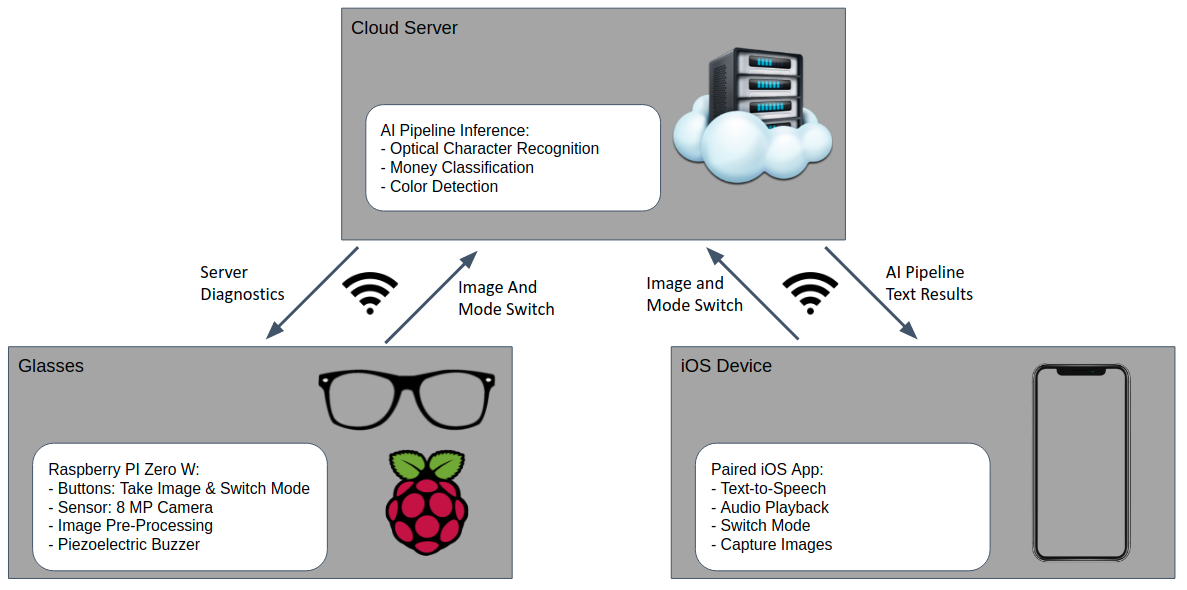
\includegraphics[scale=0.4]{img/system_diagram.png}
\caption{High-level system design diagram.}
\label{fig:system_diagram}
\end{figure}

As shown in Figure \ref{fig:system_diagram}, our design solution consists of three active components: a wearable device in the form of glasses, the user's iOS device, and a cloud server. The glasses will be the main point of interaction for a user.

The glasses will be equipped with a hardware platform consisting of a Raspberry Pi Zero W \cite{rpi-zero-w}, an 8-megapixel camera \cite{rpi-camera}, some buttons for user interaction, and a piezoelectric buzzer to play sounds to indicate processing and error states. A button on the glasses will be used to trigger the computation pipeline. The camera will be used to capture an image of the scene at which the user's head is pointed. The system will take advantage of the processor available on-board the Raspberry Pi Zero W in order to lightly process the image by scaling down its dimensions and then sending it to the server for processing. There will also be a second button connected to the Raspberry PI which allows the user to switch between modes of operation. Finally, the piezoelectric buzzer is there to allow us to send alerts to the user when some sort of error has occurred, either with the Raspberry PI or the response from the server.

The user's iOS device will be used to communicate the results of the computer vision pipeline by employing a text-to-speech engine, most likely just using Apple's native speech synthesis libraries \cite{apple-speech-synthesis}. The text will be received from the server after the processing pipeline is initiated. The iOS device will also be able to initiate the pipeline using an image taken from the device. This is simply done for convenience since it is not difficult to implement given our existing infrastructure. The user will also be able to select the operating mode from the app, using the UI interface. The app will then send the request to the server to inform it of the change. 

We initially planned to have the iOS application be used to send WiFi credentials to the on-glasses device. However, this feature is inaccessible to us without MFi certification, as it is required to gain Wireless Accessory Configuration (WAC) entitlement from Apple \cite{apple-wac}, which allows a third-party device to receive WiFi credentials from an iOS device. As a result of this constraint, it won't be possible for us to configure the glasses properly from the iOS application, and we will have to manually configure the network connection every time on the Raspberry Pi Zero W. As mentioned already, if we were to pursue this design in a scaled manufacturing capacity, we would seek MFi certification to get past this constraint and enable a better user experience.

The server will be used to run the computer vision algorithms that process the images. All communication between the server and the other devices will be done via socket communication. Upon receiving images from either the glasses or the phone, the server will process it using the currently selected computer vision algorithm and send the results to the phone for audio playback. If an error occurs during processing, the server will send an error code back to the device that initiated the processing. The server can also receive mode switch messages from either device. Upon receiving one, the current processing mode is toggled and a message is sent to the other device, informing it of the mode switch.

An example use of this system would go as follows:
\begin{enumerate}
    \item User presses a button on the eyeglasses device.
    \item Device captures a photo of the user's point of view.
    \item Device scales the photo and compresses it.
    \item Device pings the cloud server and transfers the image over WiFi.
    \item Server runs the selected computer vision pipeline on the image.
    \item Server sends the results of the computation in text form to the iOS device over WiFi.
    \item iOS device performs speech synthesis to convert text to audio and plays it through the iOS device's audio output (speakers or Bluetooth connected headphones).
\end{enumerate}

The following sections will outline the computer vision algorithms in more detail since this is what Martin worked on this term. The other components of the system (iOS app, glasses device) won't be described in detail since other members of the group were responsible for these components.

\subsection{Computer Vision Algorithms}
\label{cv-algorithms}

As previously stated, we currently support 3 different modes of operation for this device. These modes were selected based on feedback from the Lighthouse SF interview (OCR) and ease of implementation (money classification and colour detection). If time allows, we plan on adding more modes during the Winter 2022 term. This section covers the development of the algorithms for each of the modes. Note that all the code for these algorithms will be run using Python on the cloud server with the appropriate libraries.

\subsubsection{Optical Character Recognition (OCR)}
Optical Character Recognition is generally a difficult task for computer vision systems. There are currently many existing solutions available to perform OCR. During the Spring 2021 term, different OCR libraries were tested and the best library was selected to be used in the project. Please refer to our Spring 2021 report for the details of the testing. As a summary, we tested EasyOCR, PaddleOCR, Tesseract-OCR, and the Google Cloud Vision API, and found that the Google Cloud Vision API offered the best performance and the most features. This term, Python code was written to submit an API request given an input image. To accomplish this, a Google Cloud project had to be setup, and an API key was given. The images are converted to strings using base64 encoding, and the request is done using a POST request to the API server. The return from the POST request is a string containing the predictions from the API.

The API requires different operating modes for different text modalities. For machine text and handwritten text, the API suggests using DOCUMENT\_TEXT\_DETECTION mode, which is optimized for black text on white documents. For text-in-the-wild, it is suggested to use the default TEXT\_DETECTION mode, which is not optimized for documents and works for any text in general. Example results are shown in Figures \ref{fig:ocr_text-in-the-wild} and \ref{fig:ocr_handwriting} for text-in-the-wild and handwriting. As you can see, the API performs well with both input modalities. From these results, we can be assured that the API will also perform well given machine text since it is much easier in general.

\begin{figure}[H]
\centering
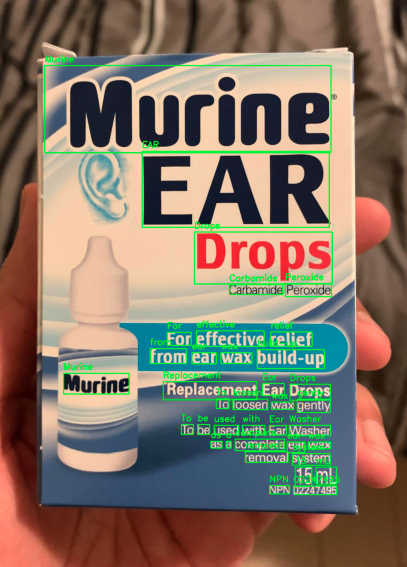
\includegraphics[scale=0.7]{img/cv_appendix/ocr_text_in_the_wild.png}
\caption{Results from the Google Cloud Vision API for an example text-in-the-wild input.}
\label{fig:ocr_text-in-the-wild}
\end{figure}

\begin{figure}[H]
\centering
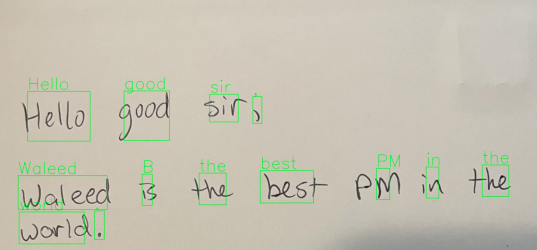
\includegraphics[scale=0.9]{img/cv_appendix/ocr_handwriting.png}
\caption{Results from the Google Cloud Vision API for an example handwriting input.}
\label{fig:ocr_handwriting}
\end{figure}

\subsubsection{Money Classification}
Money classification is the task of identifying the type of bill being shown in the image. We targeted American bills only for this task since Canadian bills have braille on them to identify the bill type. After some research, we could not find any open-source money classification algorithms already existing. Therefore, we decided to implement our own classification algorithm.

It was decided early on that a convolutional neural network (CNN) would be a good fit for this task, since these types of networks are typically very good at classifying objects based on visual patterns. The first step to having a CNN classify bills is building a dataset. To build this dataset, members of the group acquired American bills and took photos of them in various situations and orientations using their phones. The photos were saved in a folder on Google Drive and the images were separated into sub-folders, each corresponding to the type of bill. The bill types we looked to classify are the 1, 5, 10, 20, and 50 dollar bills. We tried collecting images of the bills in as many situations as possible, to ensure robustness in our classifier. Some of the possible situations we thought of are:

\begin{enumerate}
    \item Bill in center of image vs. bill closer to edge of image
    \item Nice bill vs. bill with edges folded vs. crumpled bill
    \item Holding bill in hand vs. bill resting on table/chair/floor
    \item Indoors vs. outdoors
    \item Good lighting vs. bad lighting
    \item Front side of bill vs. back side of bill
    \item Bill upside down
    \item Bill rotated
\end{enumerate}

Some example images from the dataset can be seen in Figures \ref{fig:one_dollar_nice} and \ref{fig:one_dollar_hard}. In the first image, we can see an example of a relatively easy bill to classify. In the second image, this is clearly a more difficult problem due to the bill being folded multiple times.

\begin{figure}[H]
\centering
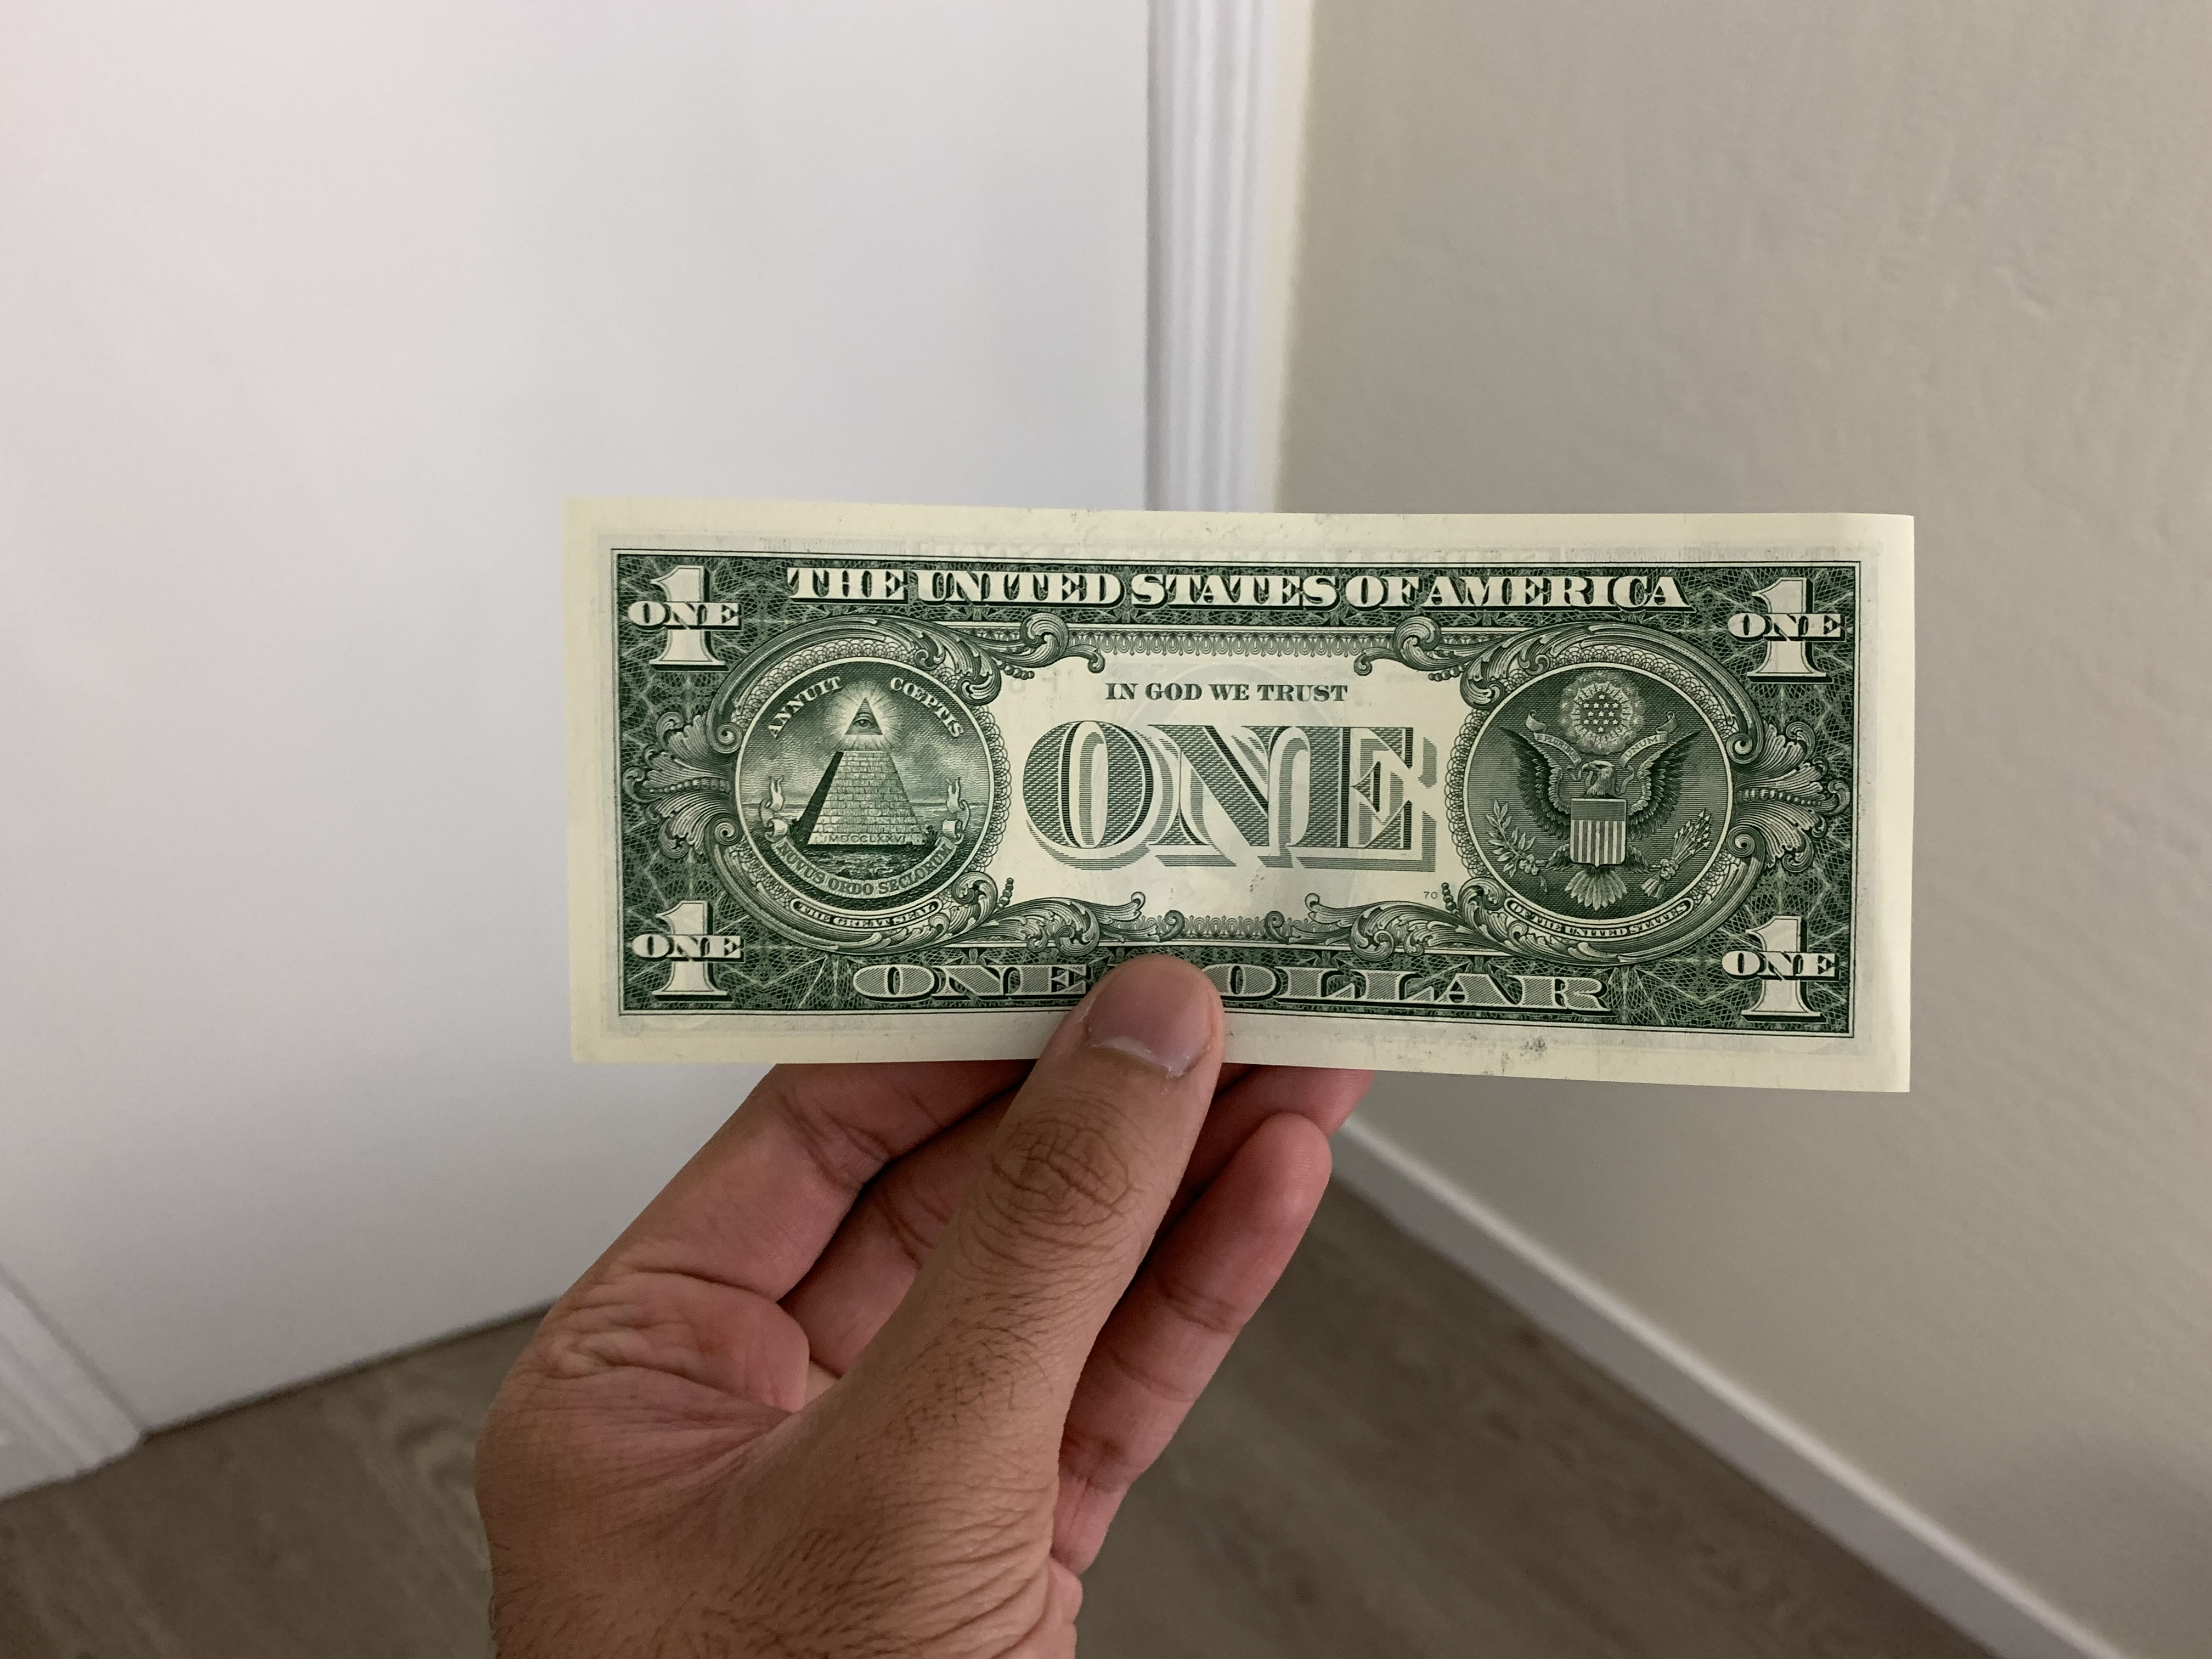
\includegraphics[scale=0.1]{img/cv_appendix/one_dollar_bill_nice.jpeg}
\caption{Easy example of a one dollar bill.}
\label{fig:one_dollar_nice}
\end{figure}

\begin{figure}[H]
\centering
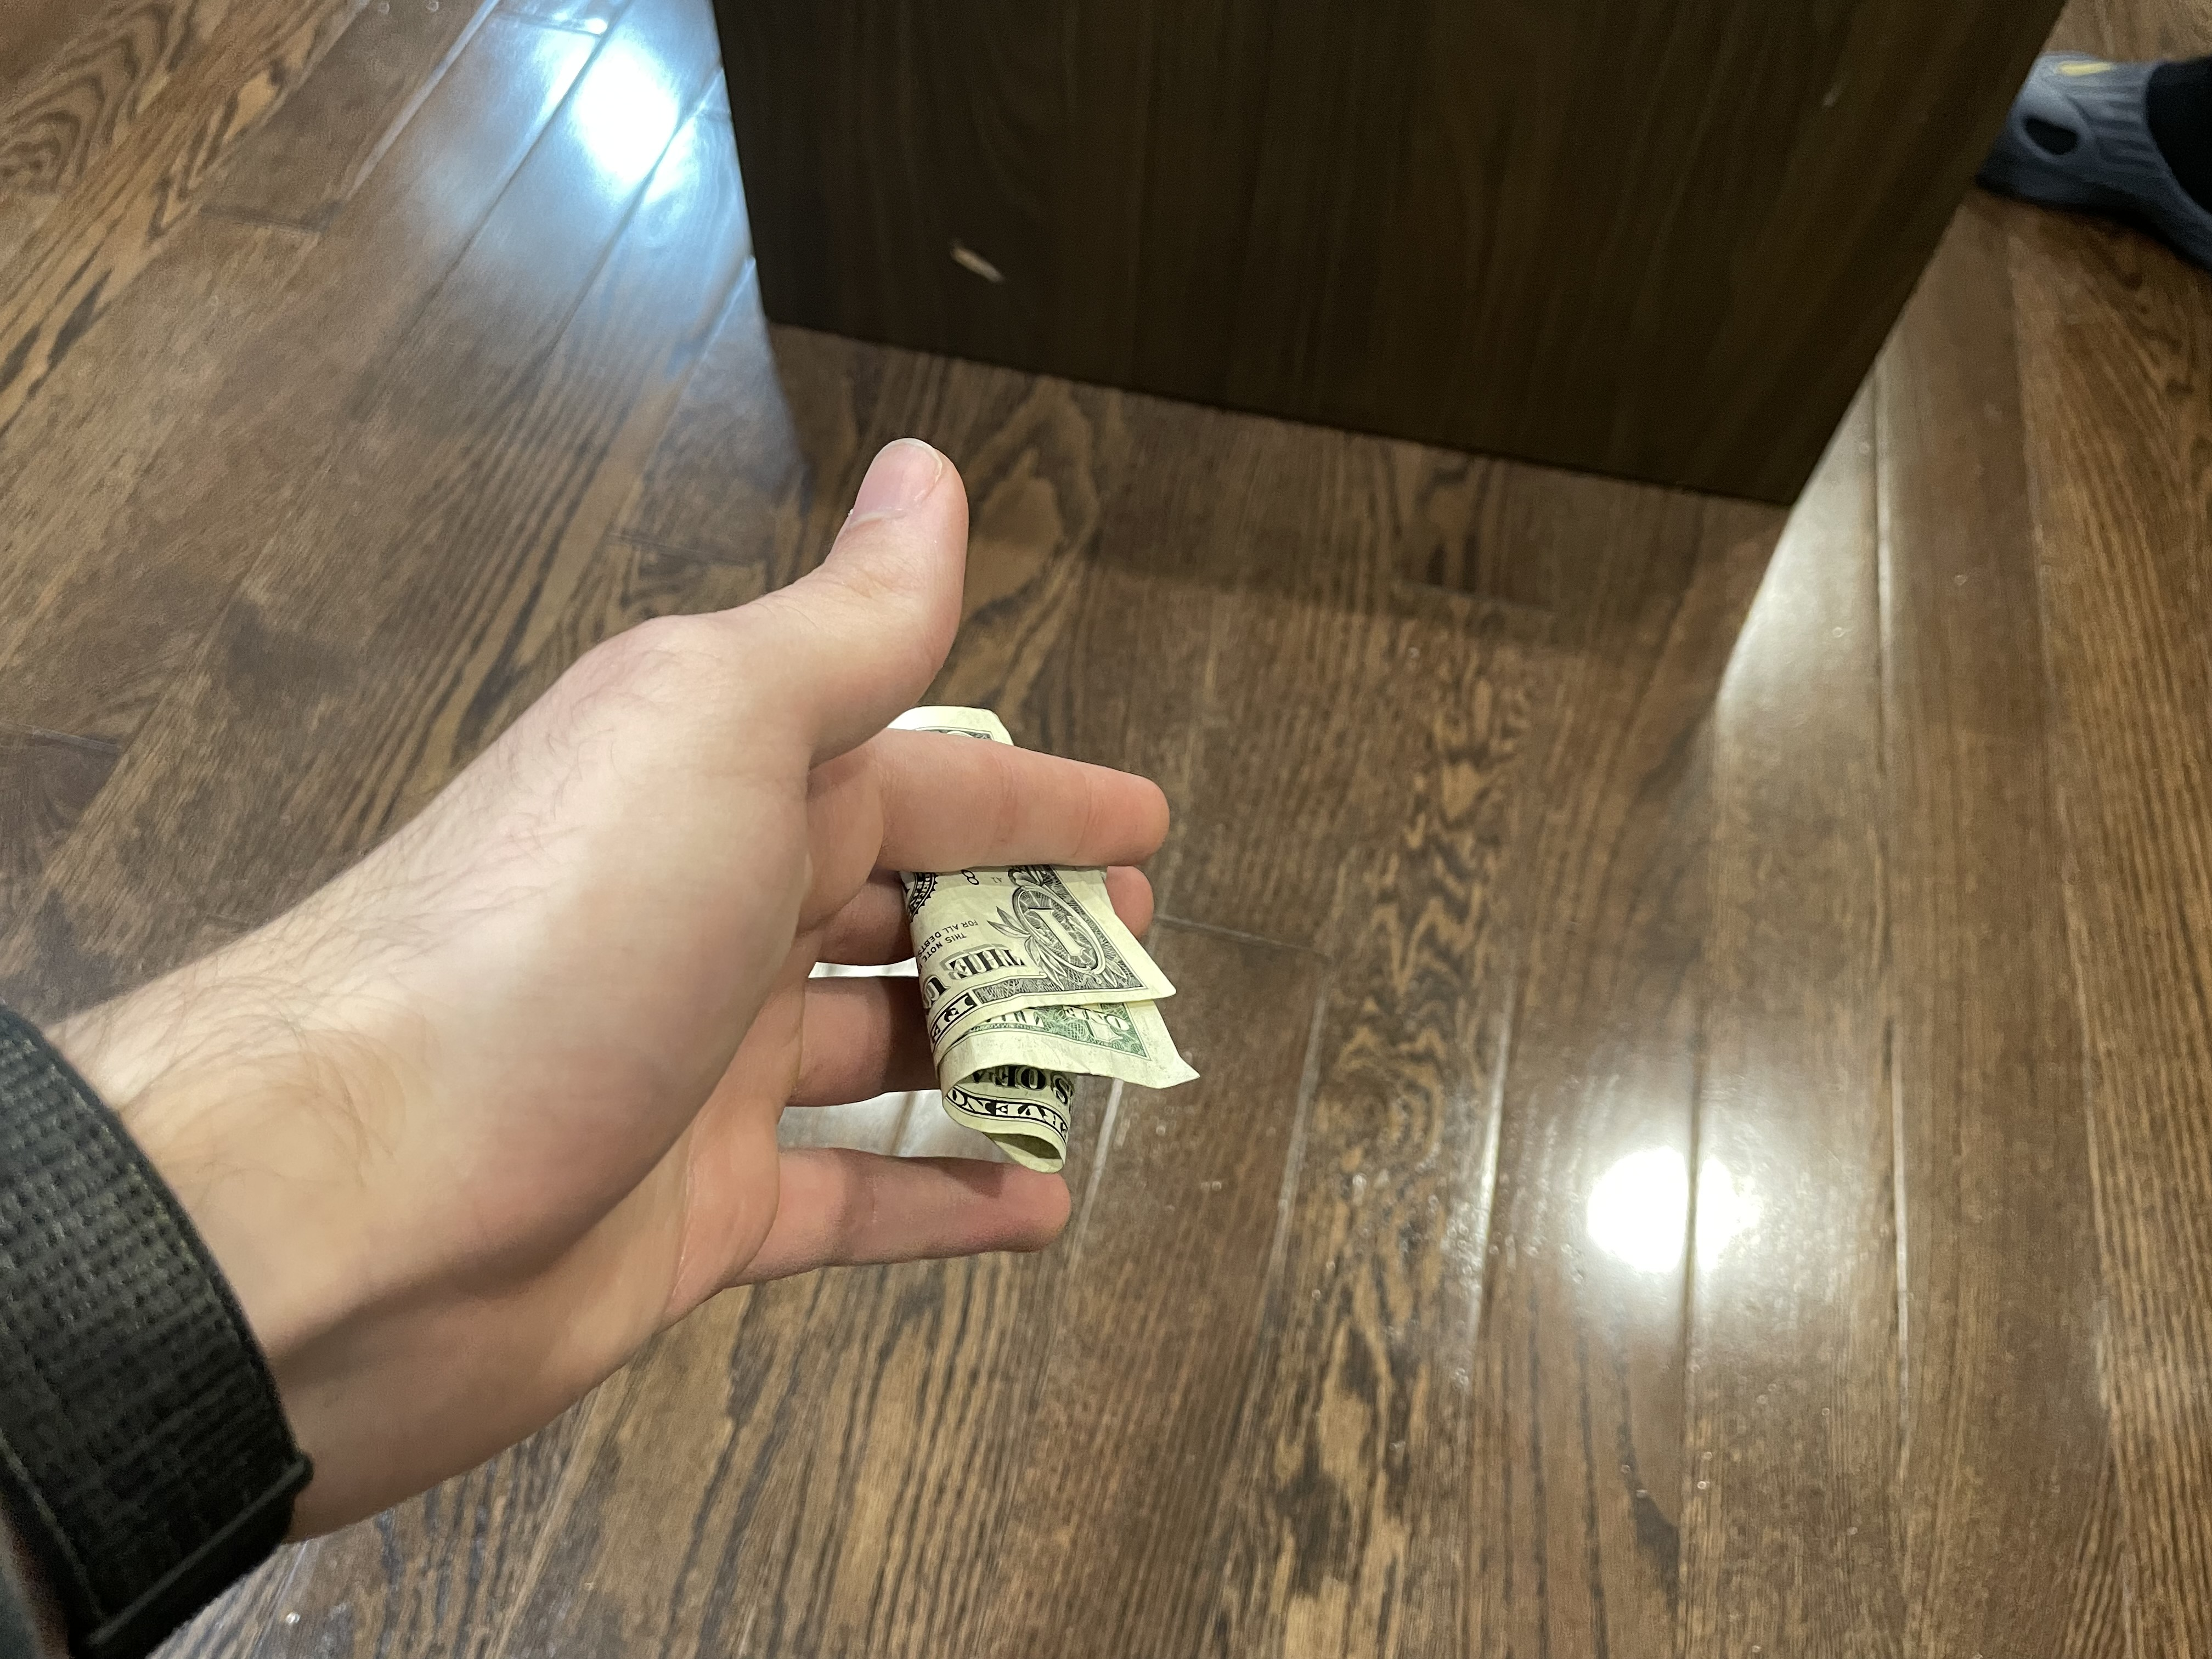
\includegraphics[scale=0.1]{img/cv_appendix/one_dollar_bill_hard.jpeg}
\caption{Difficult example of a one dollar bill.}
\label{fig:one_dollar_hard}
\end{figure}

This preliminary dataset ended up having 405 total images. To train on this dataset, it was first split into training and validation sets at a ratio of 70\% for training and 30\% for validation. The PyTorch deep learning library was then used to train a ResNet-34 CNN on this dataset. Figure \ref{fig:resnet} has a diagram showing the architecture of the ResNet-18 model. Note that the ResNet-34 is simply a scaled up version of the ResNet-18. After some hyperparameter tuning, the resulting best model achieved a validation accuracy of 94.2\%. The accuracy curves and validation confusion matrix can be seen in Figures \ref{fig:train_acc} to \ref{fig:conf_matrix}.

\begin{figure}[H]
\centering
\frame{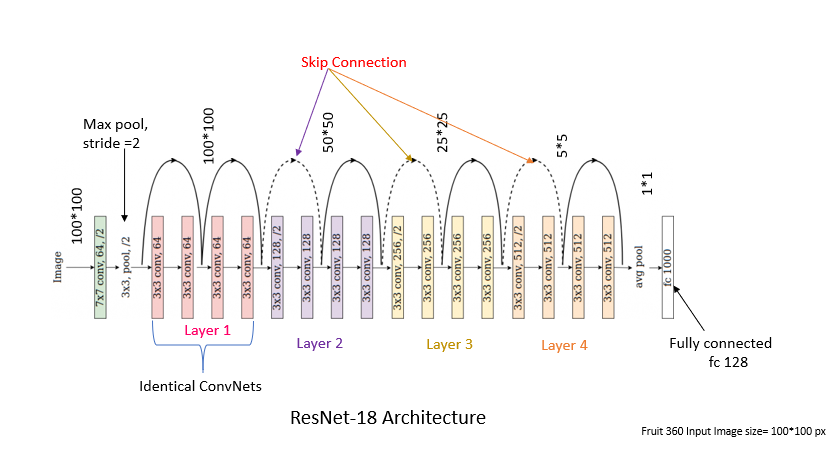
\includegraphics[scale=0.5]{img/cv_appendix/resnet18.png}}
\caption{Diagram explaining the ResNet-18 CNN architecture. \cite{resnet}}
\label{fig:resnet}
\end{figure}

\begin{figure}[H]
\centering
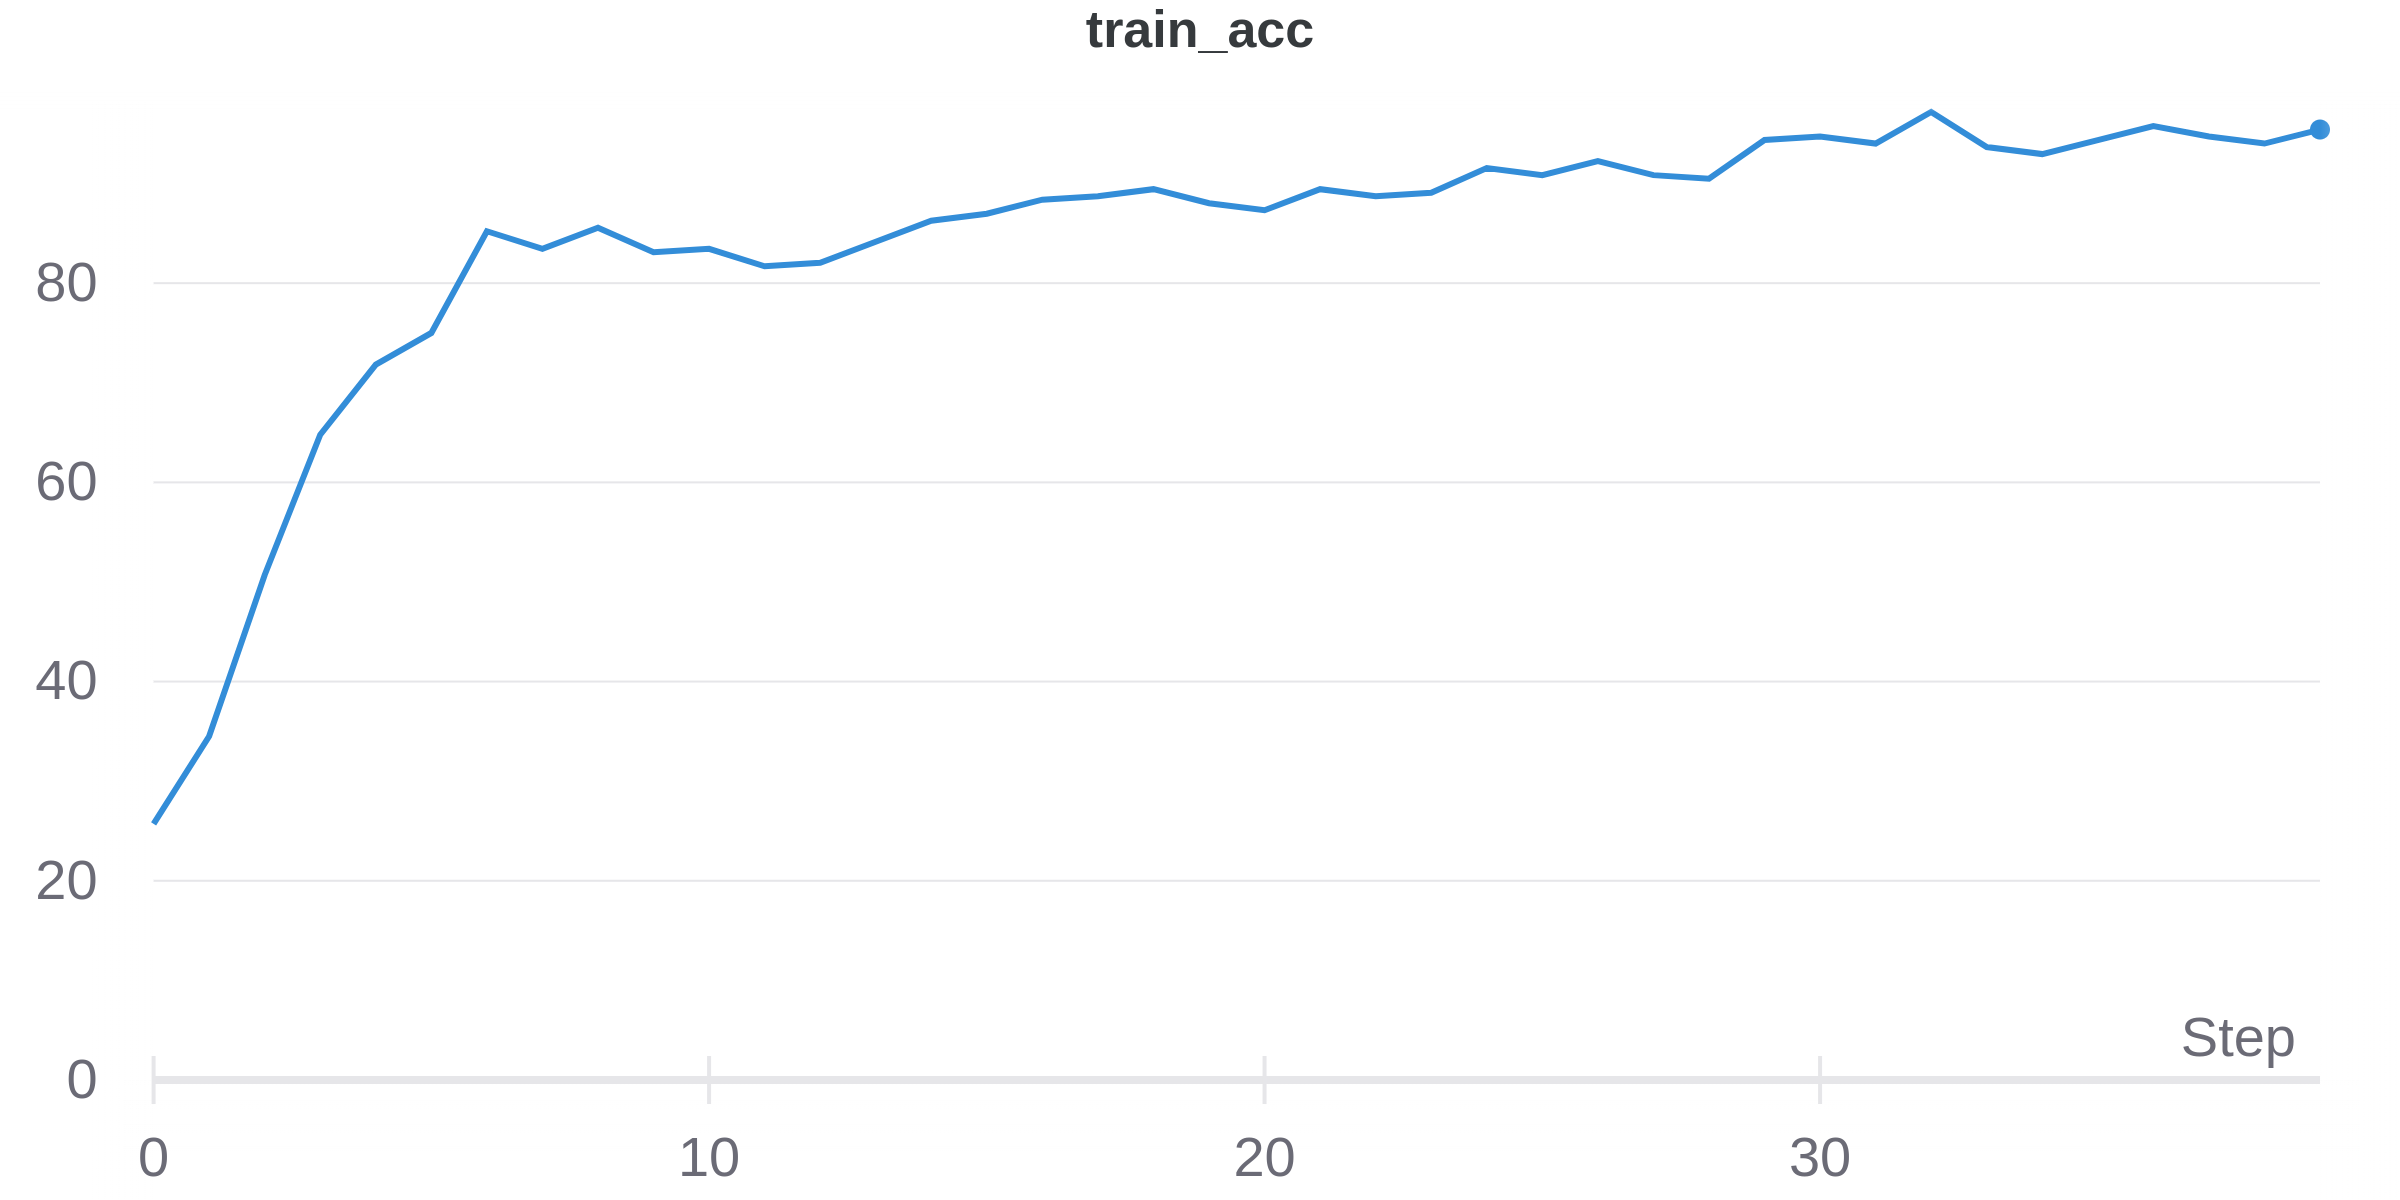
\includegraphics[scale=0.18]{img/cv_appendix/best_run_train_acc.png}
\caption{Plot of training accuracy per epoch for the best run.}
\label{fig:train_acc}
\end{figure}

\begin{figure}[H]
\centering
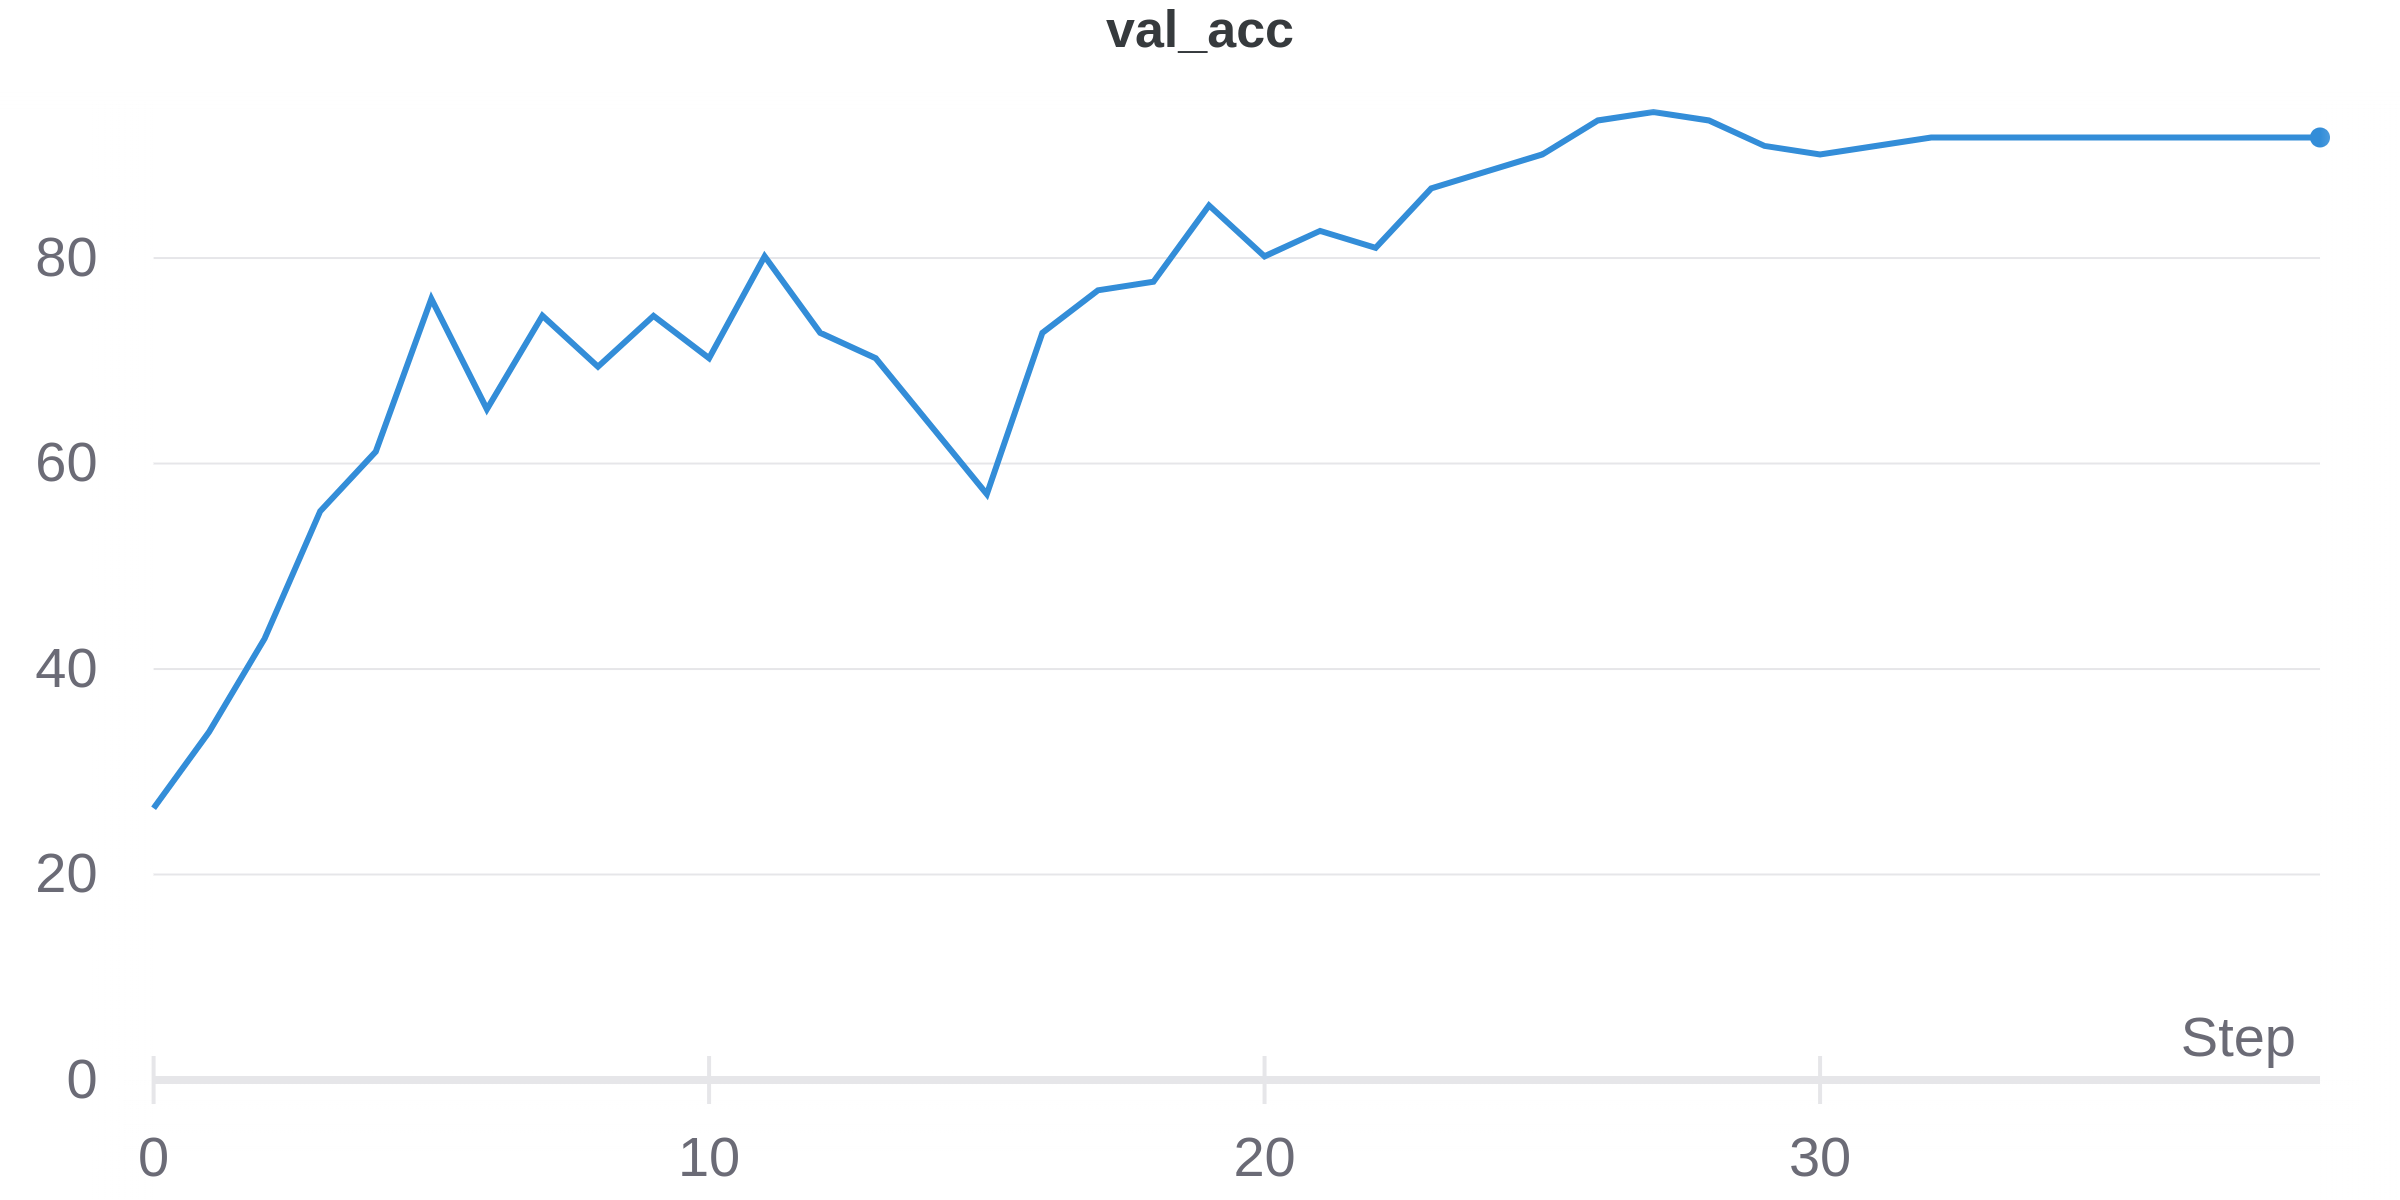
\includegraphics[scale=0.18]{img/cv_appendix/best_run_val_acc.png}
\caption{Plot of validation accuracy per epoch for the best run.}
\label{fig:val_acc}
\end{figure}

\begin{figure}[H]
\centering
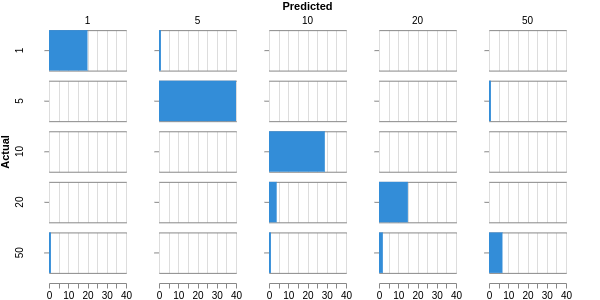
\includegraphics[scale=0.75]{img/cv_appendix/best_run_conf_matrix.png}
\caption{Confusion matrix for the best run.}
\label{fig:conf_matrix}
\end{figure}

As you can see, the classifier performs well on the given dataset. However, it could definitely be improved by collecting more training data.

\subsubsection{Colour Detection}
Colour detection is the process of identifying the most prevalent colours in front of the user. We had determined that this would be a relatively straightforward algorithm to implement and decided to work on developing one. Since our goal is to identify colours in the image by name, a database of colour names was first found. Multiple tables containing colour names and their associated RGB values were found at the following link: https://www.rapidtables.com/web/color/RGB\_Color.html. On this website, a small table with just simple colours is given, as well as a more detailed table with more colours. To identify the dominant colours in an image, a simple algorithm would be to assign each pixel in the image to its closest colour in the database by taking the euclidean distance between that pixel's RGB value and every colour in the database. We can then simply assign the database colour with the smallest distance value to that pixel. The equation for the euclidean distance can be seen in Equation \ref{eq:euclidean_dist}, where $d_i$ is the distance to the $i_{th}$ colour in the database. 

\begin{equation}
\label{eq:euclidean_dist}
d_i=\sqrt{(R - R_i)^2 + (G - G_i)^2 + (B - B_i)^2}
\end{equation}

Doing this with pure Python loops results in extremely slow computation times. However, using the NumPy library allows the algorithm to be very quick, less than a second for a 200x200 image. Once a database colour is assigned to each pixel, we can simply count the number of pixels corresponding to each database colour and return the top 3 colours with the highest pixel counts. Example results on a few test images using the small colour database can be found in Figures \ref{fig:lego_small} to \ref{fig:drops_small}. These results also have the reconstructed image, where the colour of each pixel is the corresponding database colour.

\begin{figure}[H]
\centering
\frame{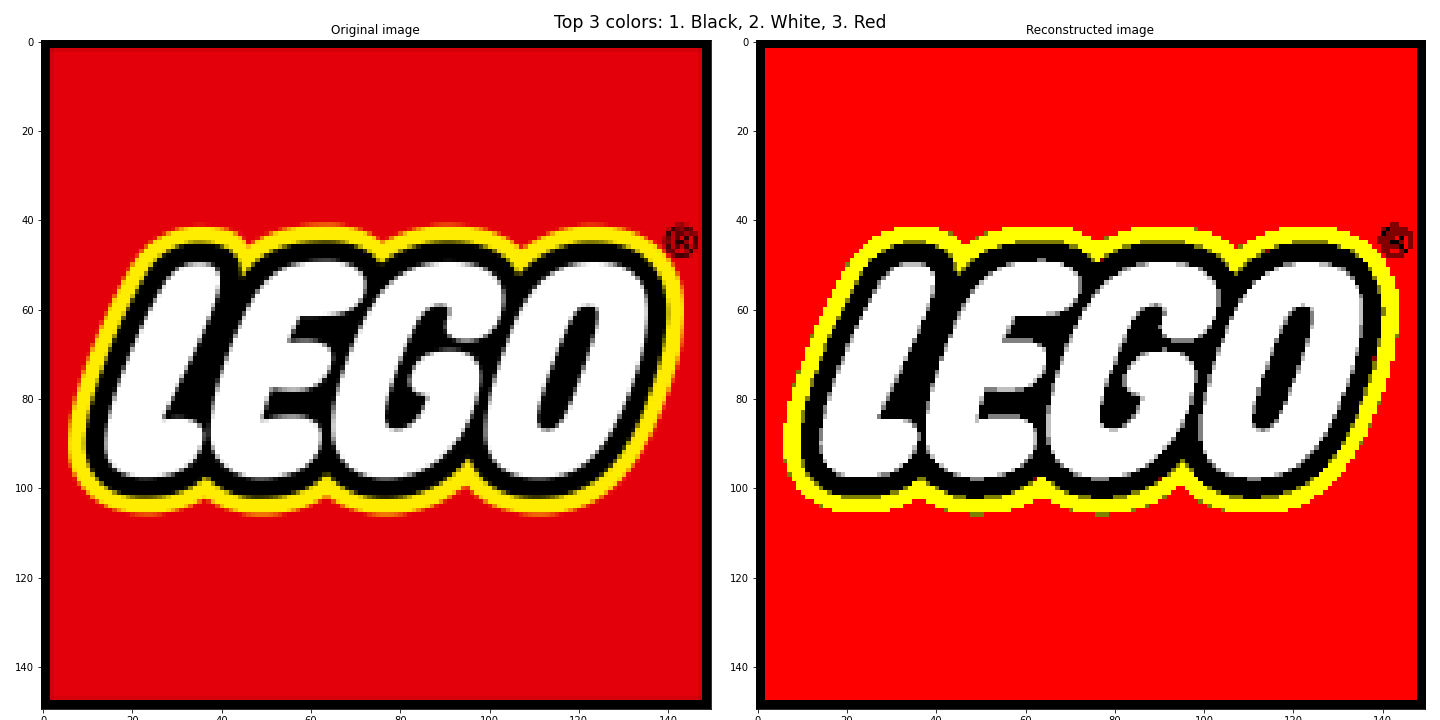
\includegraphics[scale=0.32]{img/cv_appendix/lego_small.png}}
\caption{Colour detection result on lego logo using small colour database.}
\label{fig:lego_small}
\end{figure}

\begin{figure}[H]
\centering
\frame{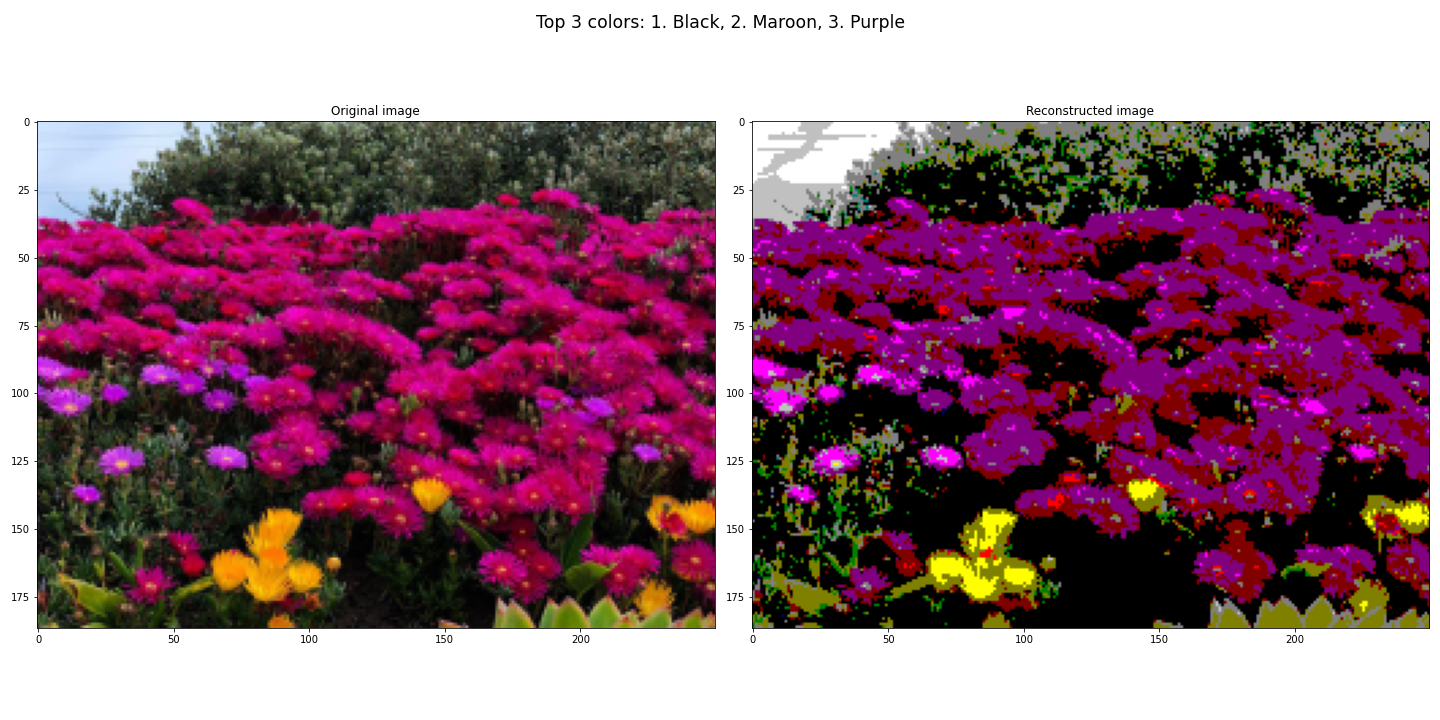
\includegraphics[scale=0.32]{img/cv_appendix/flowers_small.png}}
\caption{Colour detection result on flowers using small colour database.}
\label{fig:flowers_small}
\end{figure}

\begin{figure}[H]
\centering
\frame{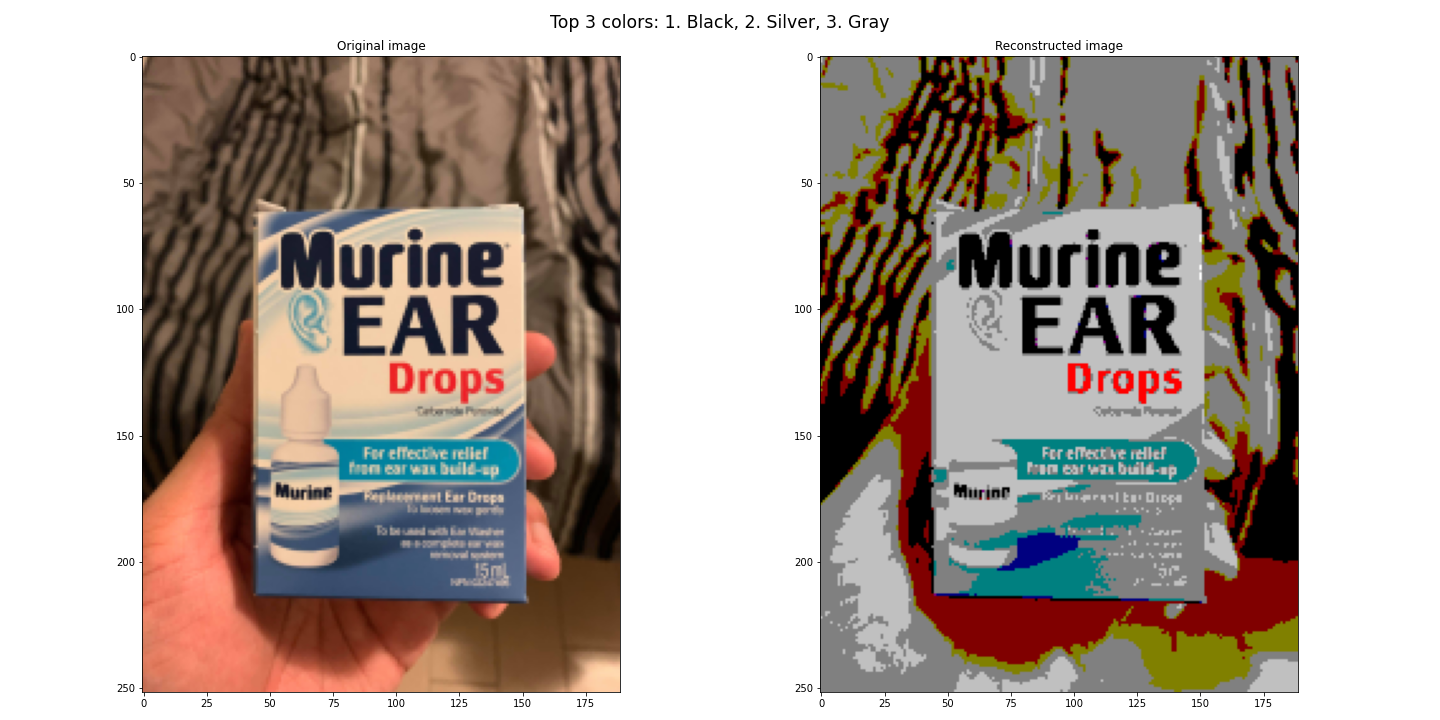
\includegraphics[scale=0.32]{img/cv_appendix/drops_small.png}}
\caption{Colour detection result on ear drops box using small colour database.}
\label{fig:drops_small}
\end{figure}

Looking at the reconstructed results, it is clear that this small colour database is not detailed enough to accurately describe the more complex images. The same images were then processed with the larger database. The results can be seen in Figures \ref{fig:lego_medium} to \ref{fig:drops_medium}.

\begin{figure}[H]
\centering
\frame{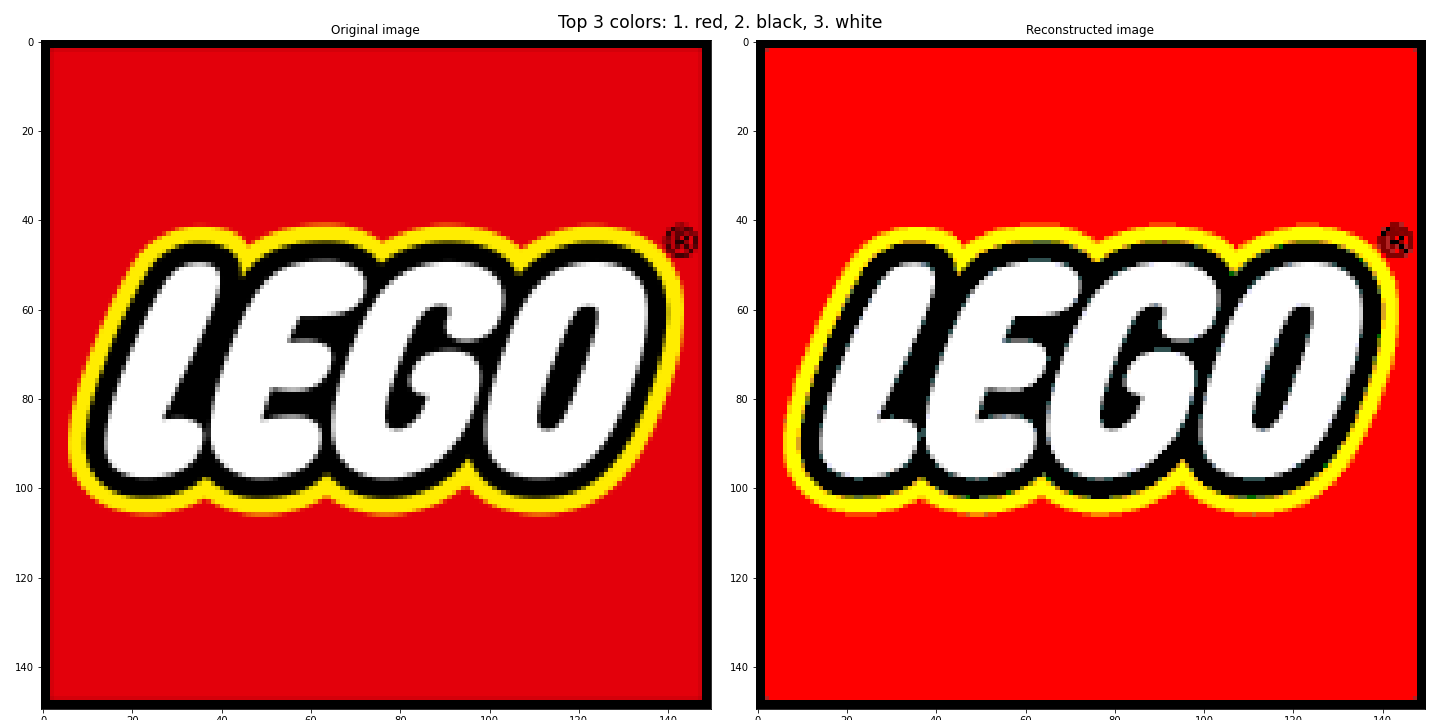
\includegraphics[scale=0.32]{img/cv_appendix/lego_medium.png}}
\caption{Colour detection result on lego logo using larger colour database.}
\label{fig:lego_medium}
\end{figure}

\begin{figure}[H]
\centering
\frame{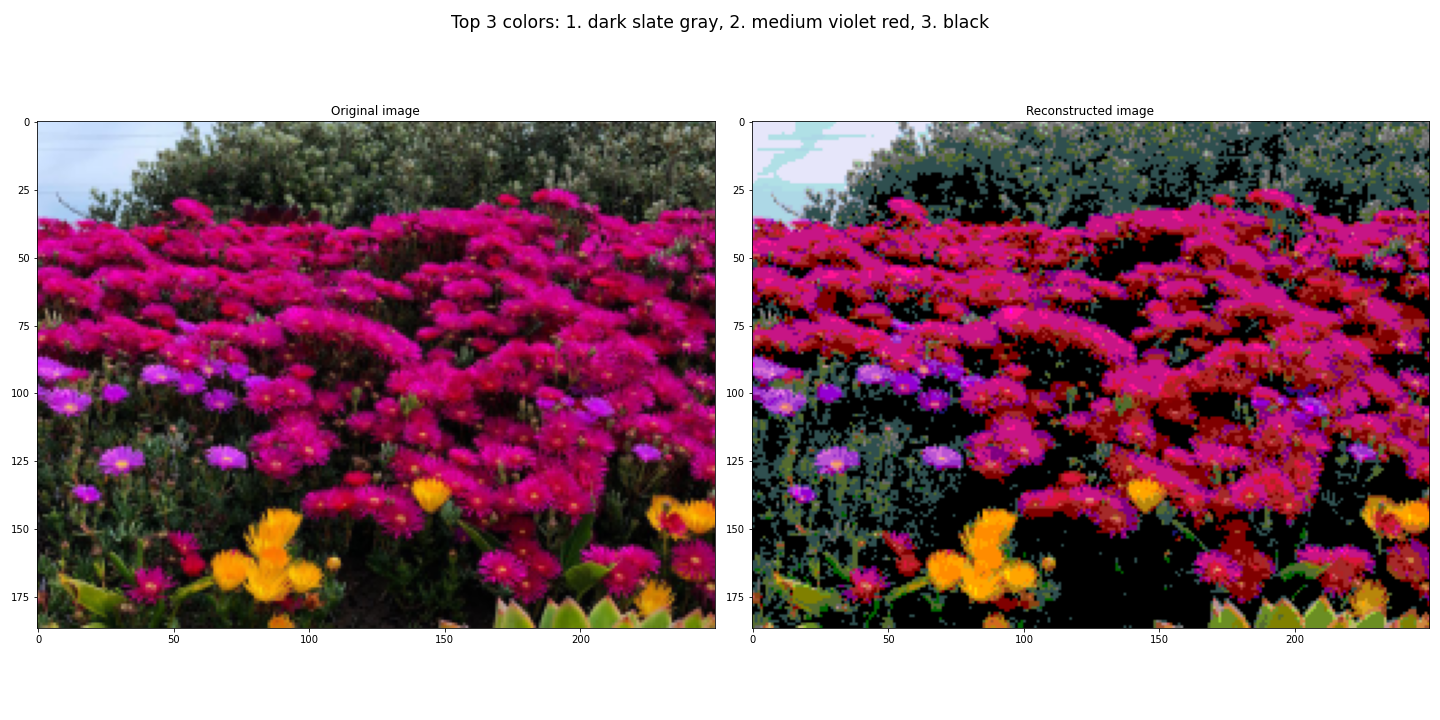
\includegraphics[scale=0.32]{img/cv_appendix/flowers_medium.png}}
\caption{Colour detection result on flowers using larger colour database.}
\label{fig:flowers_medium}
\end{figure}

\begin{figure}[H]
\centering
\frame{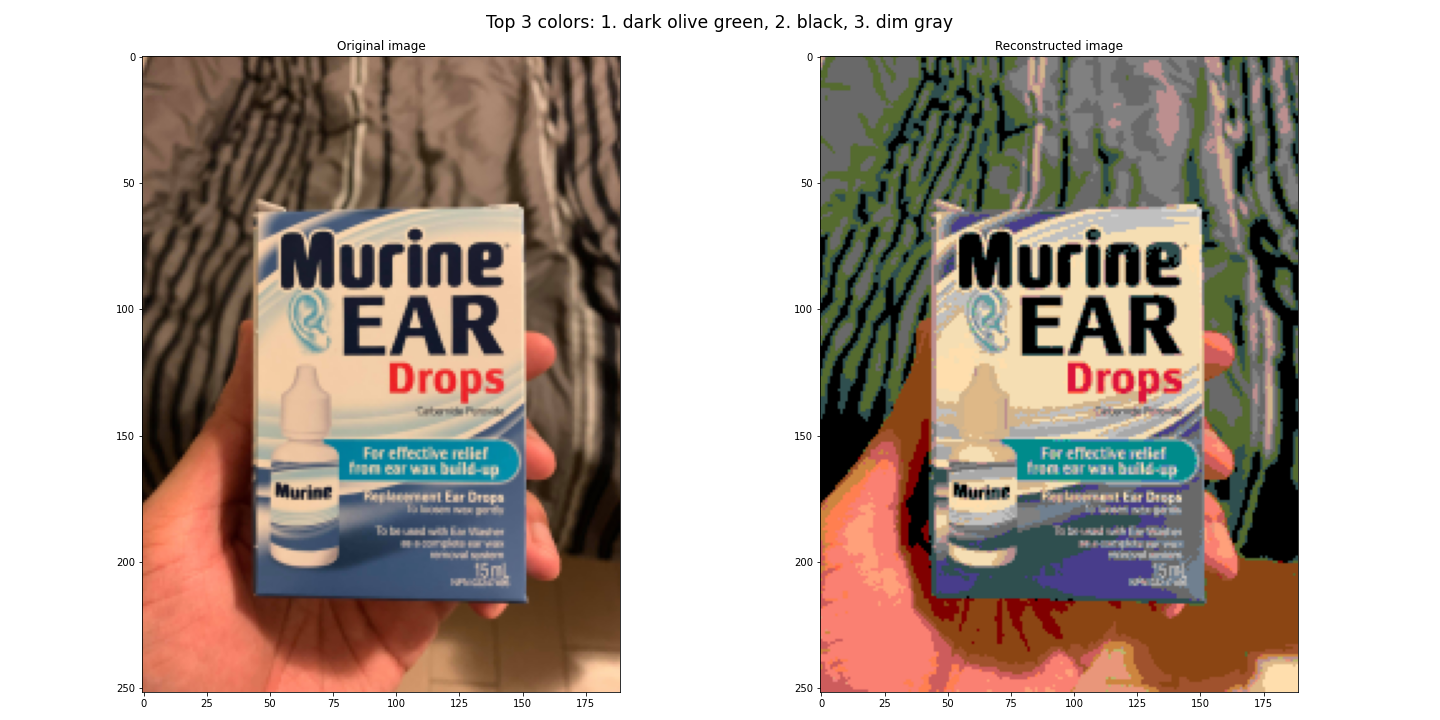
\includegraphics[scale=0.32]{img/cv_appendix/drops_medium.png}}
\caption{Colour detection result on ear drops box using larger colour database.}
\label{fig:drops_medium}
\end{figure}

Clearly, the larger database is necessary for good performance on real-life images. However, there still exists the issue of the algorithm reporting background pixel colours. For example, in Figure \ref{fig:flowers_medium}, two of the top three colours are dark slate grey and black, which are more prevalent in the background. Ideally, the user would probably want to know the colours of the flowers in this case. Either performing background segmentation or simply looking at the middle of the image might help with this issue, but these methods have not been explored yet.

\newpage
\begin{landscape}
    \subsection{Engineering Design Specification}
    \subsubsection{v0.1}
    \begin{center}
        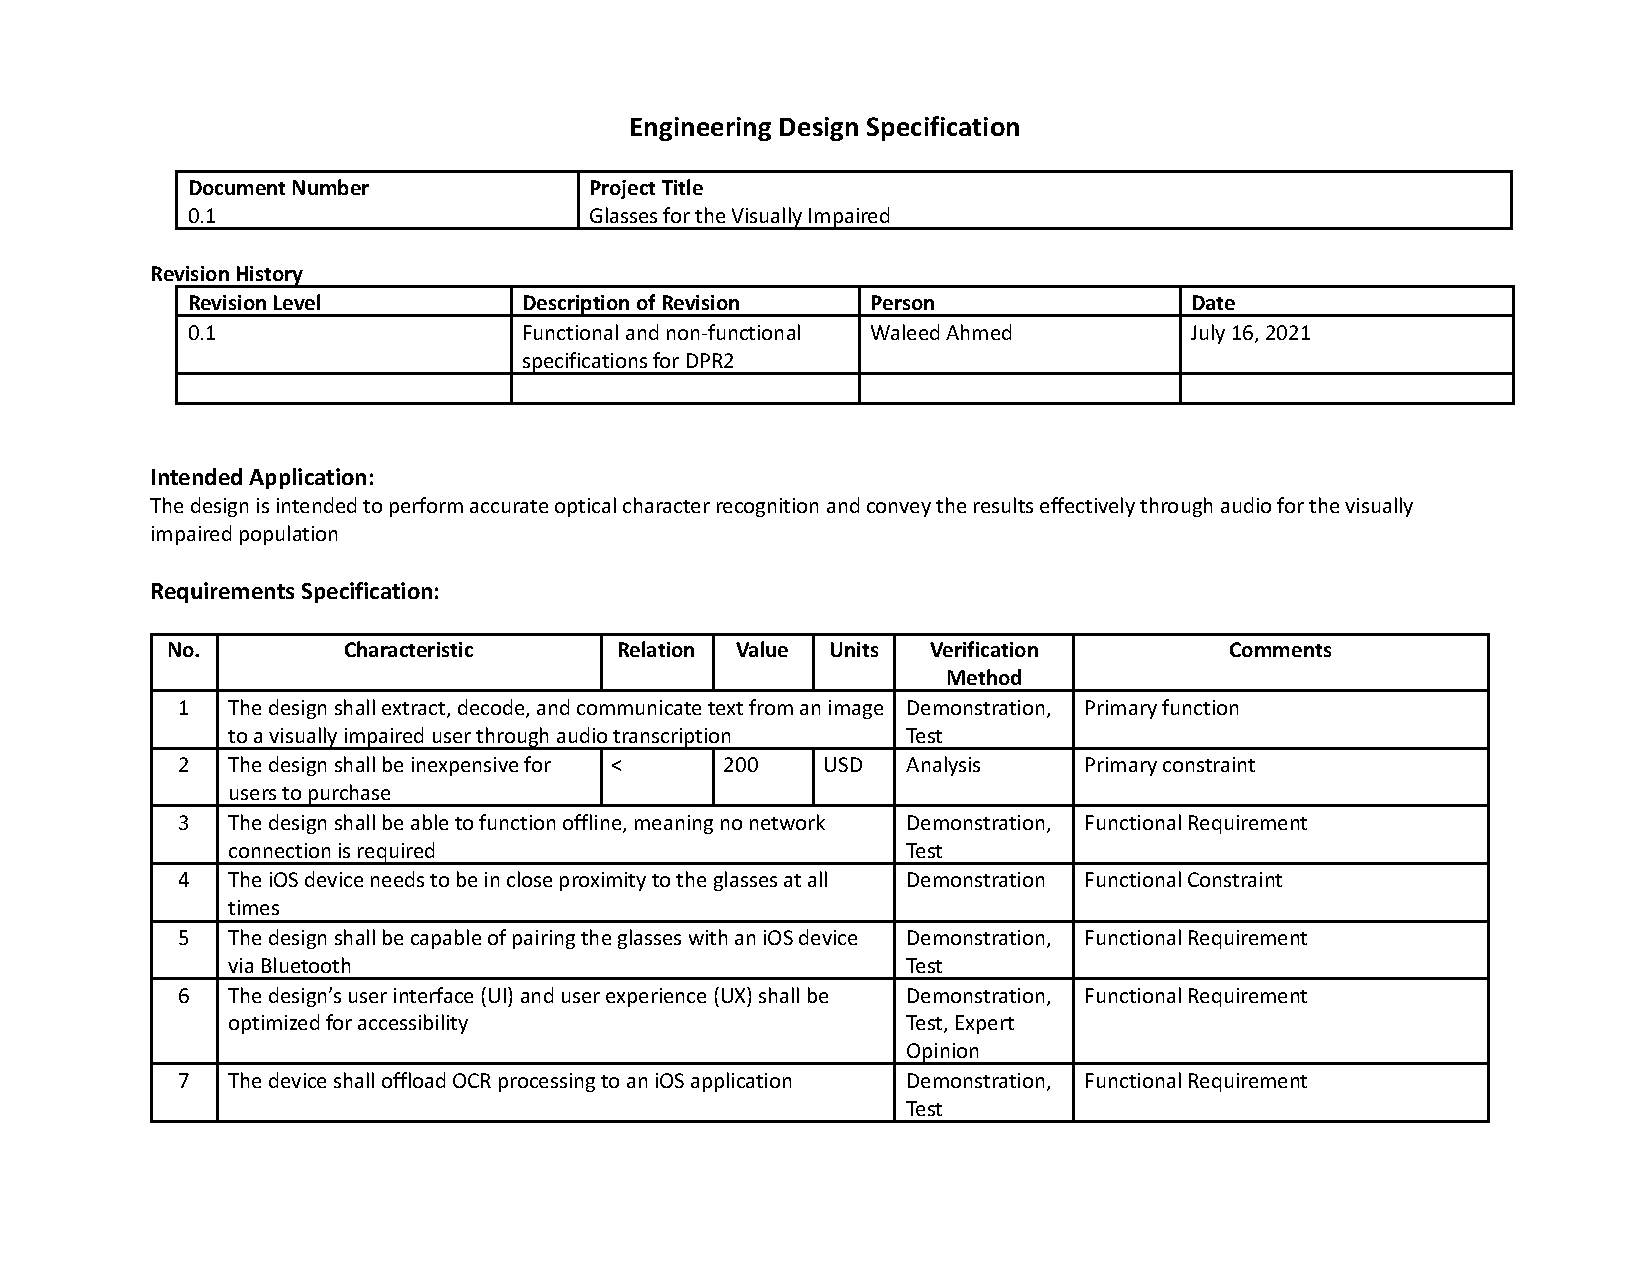
\includegraphics[page=1,width={0.86\linewidth}]{pdf/eds_0.1.pdf}
        \newpage
        \includegraphics[page=2,width={0.86\linewidth}]{pdf/eds_0.1.pdf}
    \end{center}
    
    \newpage
    \subsubsection{v0.2}
    \label{eds-0.2}
    \begin{center}
        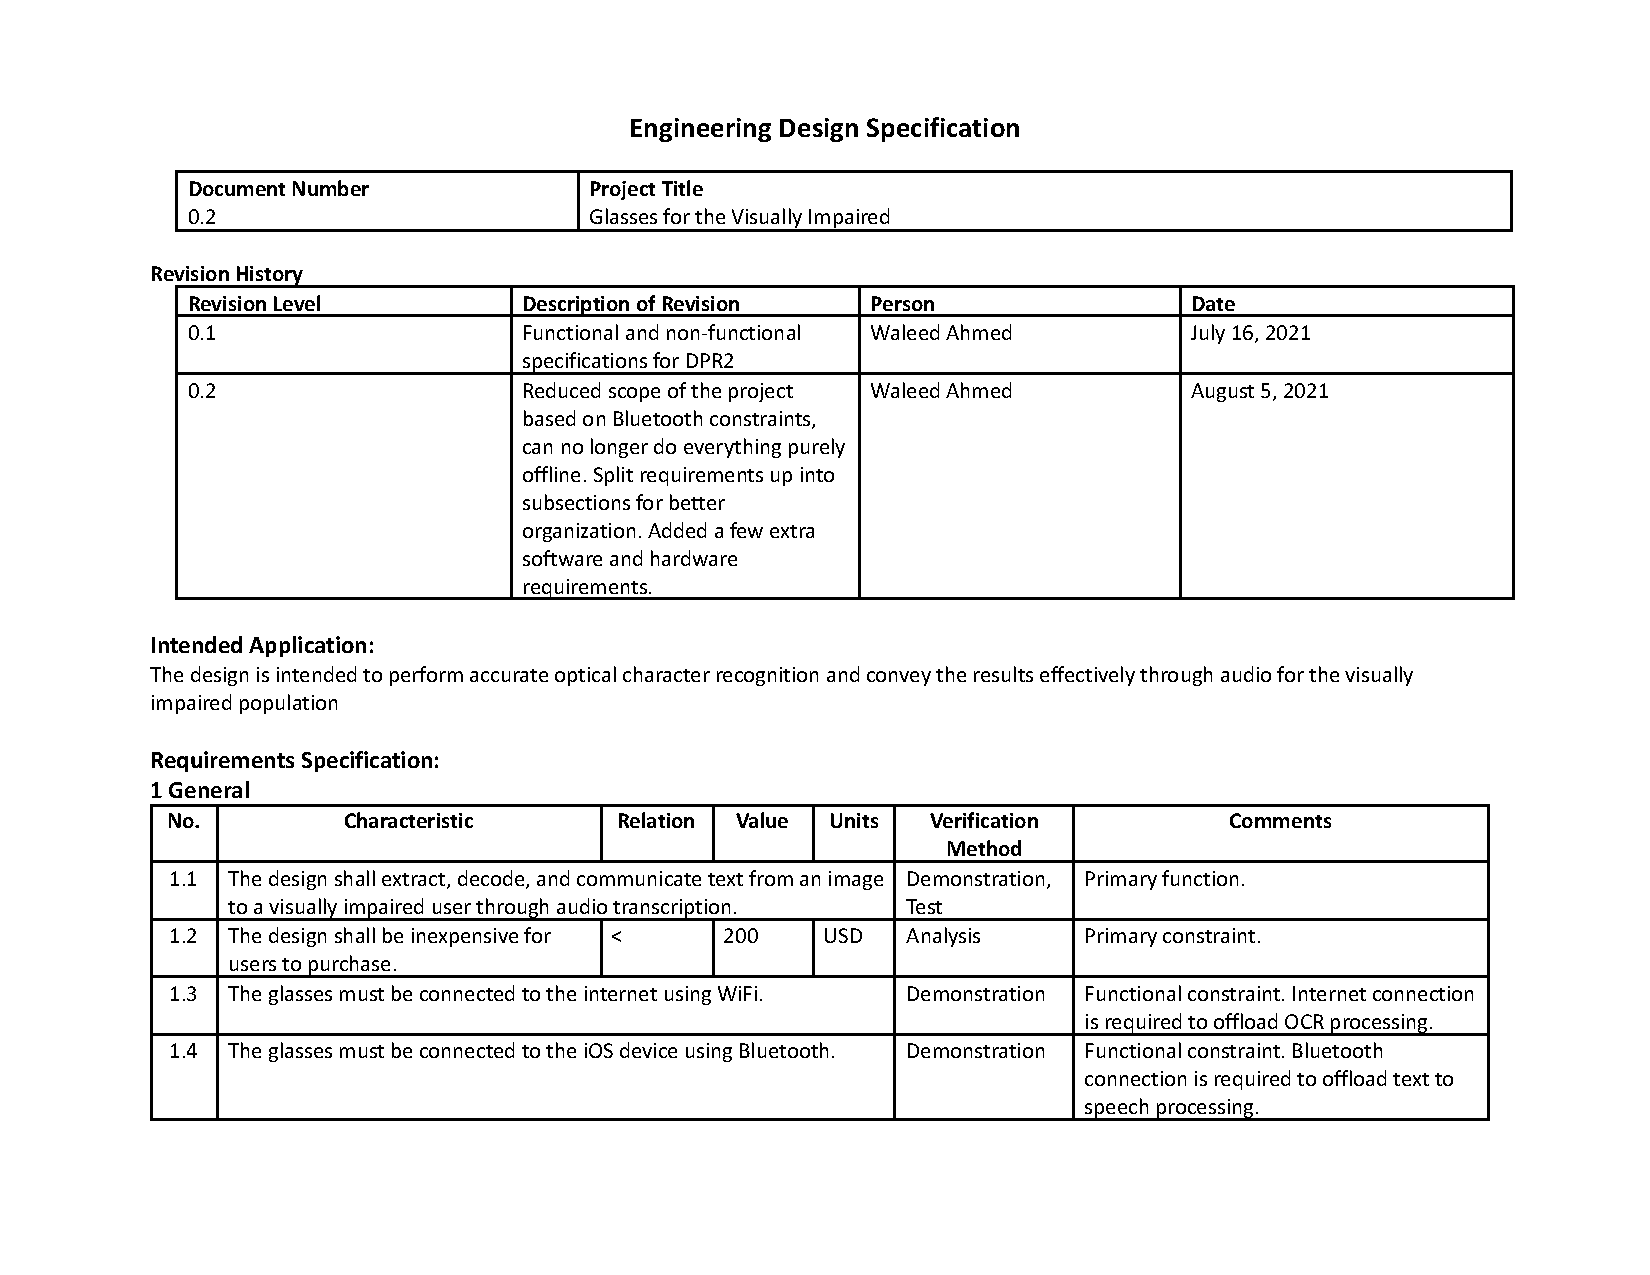
\includegraphics[page=1,width={0.86\linewidth}]{pdf/eds_0.2.pdf}
        \newpage
        \includegraphics[page=2,width={0.86\linewidth}]{pdf/eds_0.2.pdf}
        \newpage
        \includegraphics[page=3,width={0.86\linewidth}]{pdf/eds_0.2.pdf}
    \end{center}
    
    \newpage
    \subsubsection{v0.3}
    \label{eds-0.3}
    \begin{center}
        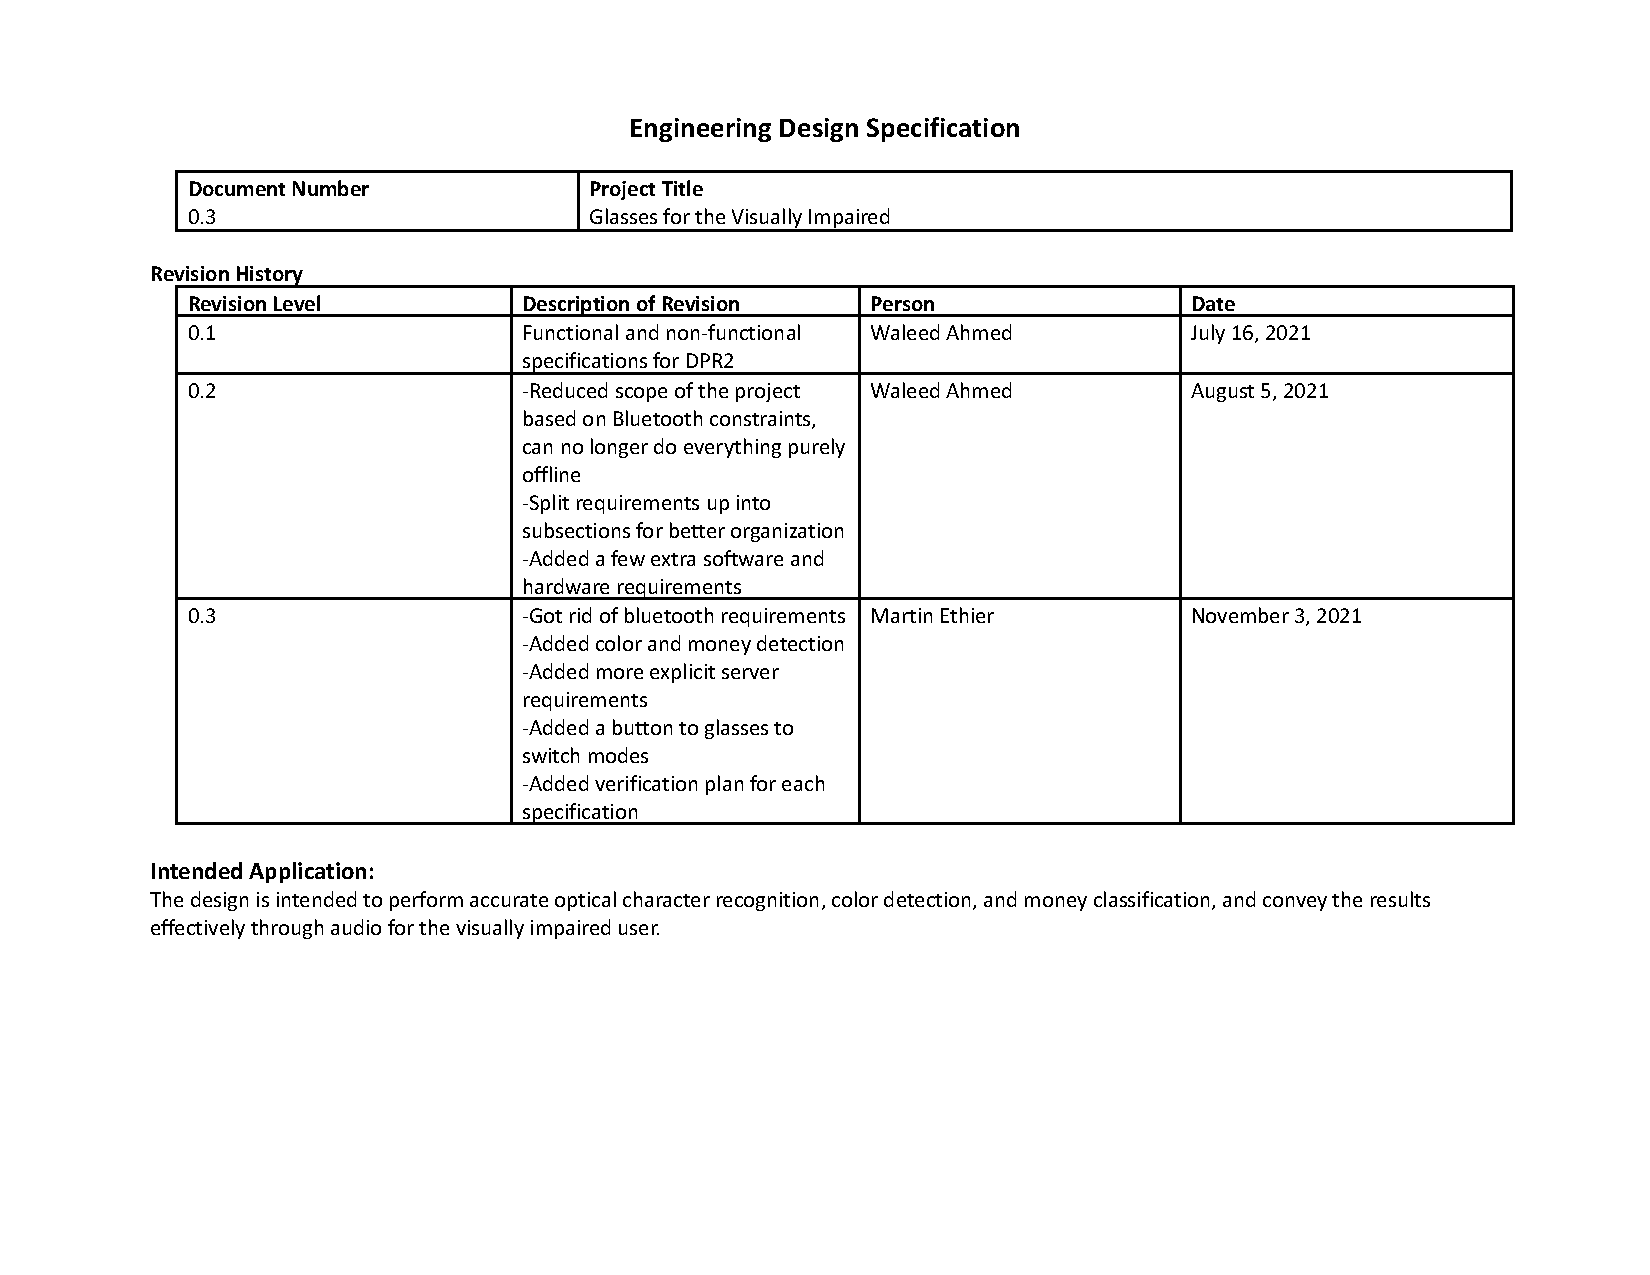
\includegraphics[page=1,width={0.86\linewidth}]{pdf/eds_v0.3.pdf}
        \newpage
        \includegraphics[page=2,width={0.86\linewidth}]{pdf/eds_v0.3.pdf}
        \newpage
        \includegraphics[page=3,width={0.86\linewidth}]{pdf/eds_v0.3.pdf}
        \newpage
        \includegraphics[page=4,width={0.86\linewidth}]{pdf/eds_v0.3.pdf}
        \newpage
        \includegraphics[page=5,width={0.86\linewidth}]{pdf/eds_v0.3.pdf}
    \end{center}
\end{landscape}

\newpage
\section{Appendix B - Verification and Validation Data}

\subsection{Algorithm Testing Datasets}
In order to properly verify the performance of the computer vision algorithms we deploy, we plan on building custom testing datasets for each modality. These datasets will be collected using both the Raspberry PI camera that is used on the device and the iPhone camera, to ensure the algorithms are robust to both inputs. For each dataset, specific target use cases have been identified. The images in each of these datasets will be chosen to reflect these use cases. Note that the list of identified use cases can grow over time as we identify more of them. Evaluation metrics have also been defined for each dataset. Also note that we have not started collection of any of these datasets, as we are waiting for all members to be on campus to assist in image collection. This work will be done during the Winter 2022 term.

\subsubsection{Machine Text Dataset}
To evaluate our OCR performance on machine text, a dataset will be collected which encompasses the following identified use cases:

\begin{enumerate}
    \item Books
    \item Text on computer monitors
    \item Printed documents
\end{enumerate}

The metric used to evaluate will be Word Error Rate (WER), which is commonly used in text recognition. An explanation of WER can be found in Appendix D. We have set the WER goal to 10\% (lower is better), since this is the threshold most OCR libraries fall under.

\subsubsection{Handwritten Text Dataset}
To evaluate our OCR performance on handwritten text, a dataset will be collected which encompasses the following identified use cases:

\begin{enumerate}
    \item Printed letters
    \item Printed class notes
    \item Class notes on computer monitors
    \item General household lists (groceries, chores, etc...)
\end{enumerate}

The metric used to evaluate will also be Word Error Rate (WER), since this is still a text recognition task. An explanation of WER can be found in Appendix D. We have set the WER goal to 25\% (lower is better), since handwritten text is generally much more difficult than machine text due to the high variability from person to person. It will also be important to collect this dataset with as many different handwriting styles as possible.

\subsubsection{Text-in-the-wild Dataset}
To evaluate our OCR performance on text-in-the-wild, a dataset will be collected which encompasses the following identified use cases:

\begin{enumerate}
    \item Store and restaurant signs
    \item Traffic signs
    \item Way finding signs (such as uWaterloo building signs)
    \item Packages
\end{enumerate}

The metric used to evaluate will be F-score, which is more commonly used for object detection. Since a difficult aspect of text-in-the-wild OCR is the detection of the text, we need a metric that takes this into account. An explanation of F-score can be found in Appendix D. We have set the F-score goal to 60\% (higher is better), since this seemed to be a common number for many text-in-the-wild benchmarks.

\subsubsection{Money Classification Dataset}
Money classification is more straightforward to evaluate than OCR. We did not see the need to define use cases for this task since it is always the same use case: classifying money. We will build this test set to try and capture as much variability in the dataset as possible. Examples of these variabilities are outlined in Section 13.2.2. The metric used to evaluate will simply be accuracy, since this is the most commonly used metric for classification. We have set the goal accuracy to 90\%, as we felt this was a reachable number.

\subsubsection{Colour Detection Dataset}
We have identified the following use cases for colour detection:

\begin{enumerate}
    \item Clothing
    \item Flowers
    \item Crayons, pencils, and markers
\end{enumerate}

The metric used to evaluate will once again be accuracy. We will collect test images and label the images with the top 3 colours we would would describe the image with. We have set the goal accuracy to 90\%, as we felt this was a reachable number.

\section{Appendix C - Design Project Management Data}
\label{appendix-c}

\subsection{Summary of Software and Tools Used}
We are using many tools for configuration management and record keeping. They are all listed below:

\begin{itemize}
    \item Discord: Internal meetings and communication.
    \item Notion: Meeting and research notes. See Section \ref{meeting-logs} for more on our Notion setup.
    \item ClickUp: Tasks and timelines. See Section \ref{schedule} for more info.
    \item Overleaf: LaTeX editor to create and store reports.
    \item Google Drive: Store files, datasets, presentation slides, and revision controlled documents such as the engineering design specification and risk register.
    \item Github: Source code and software documentation.
    \item Microsoft Teams: Meetings with faculty advisor.
\end{itemize}

\subsection{Schedule}
\label{schedule}
Below is the Gantt charts showcasing the current high level timeline. It is then followed by Gantt charts for the subsystem level tasks for the server software, the iOS software, AI software, and hardware. Note that these will be continually evolving as our project progresses, this is just a current snapshot of where we are at.
\begin{center}
    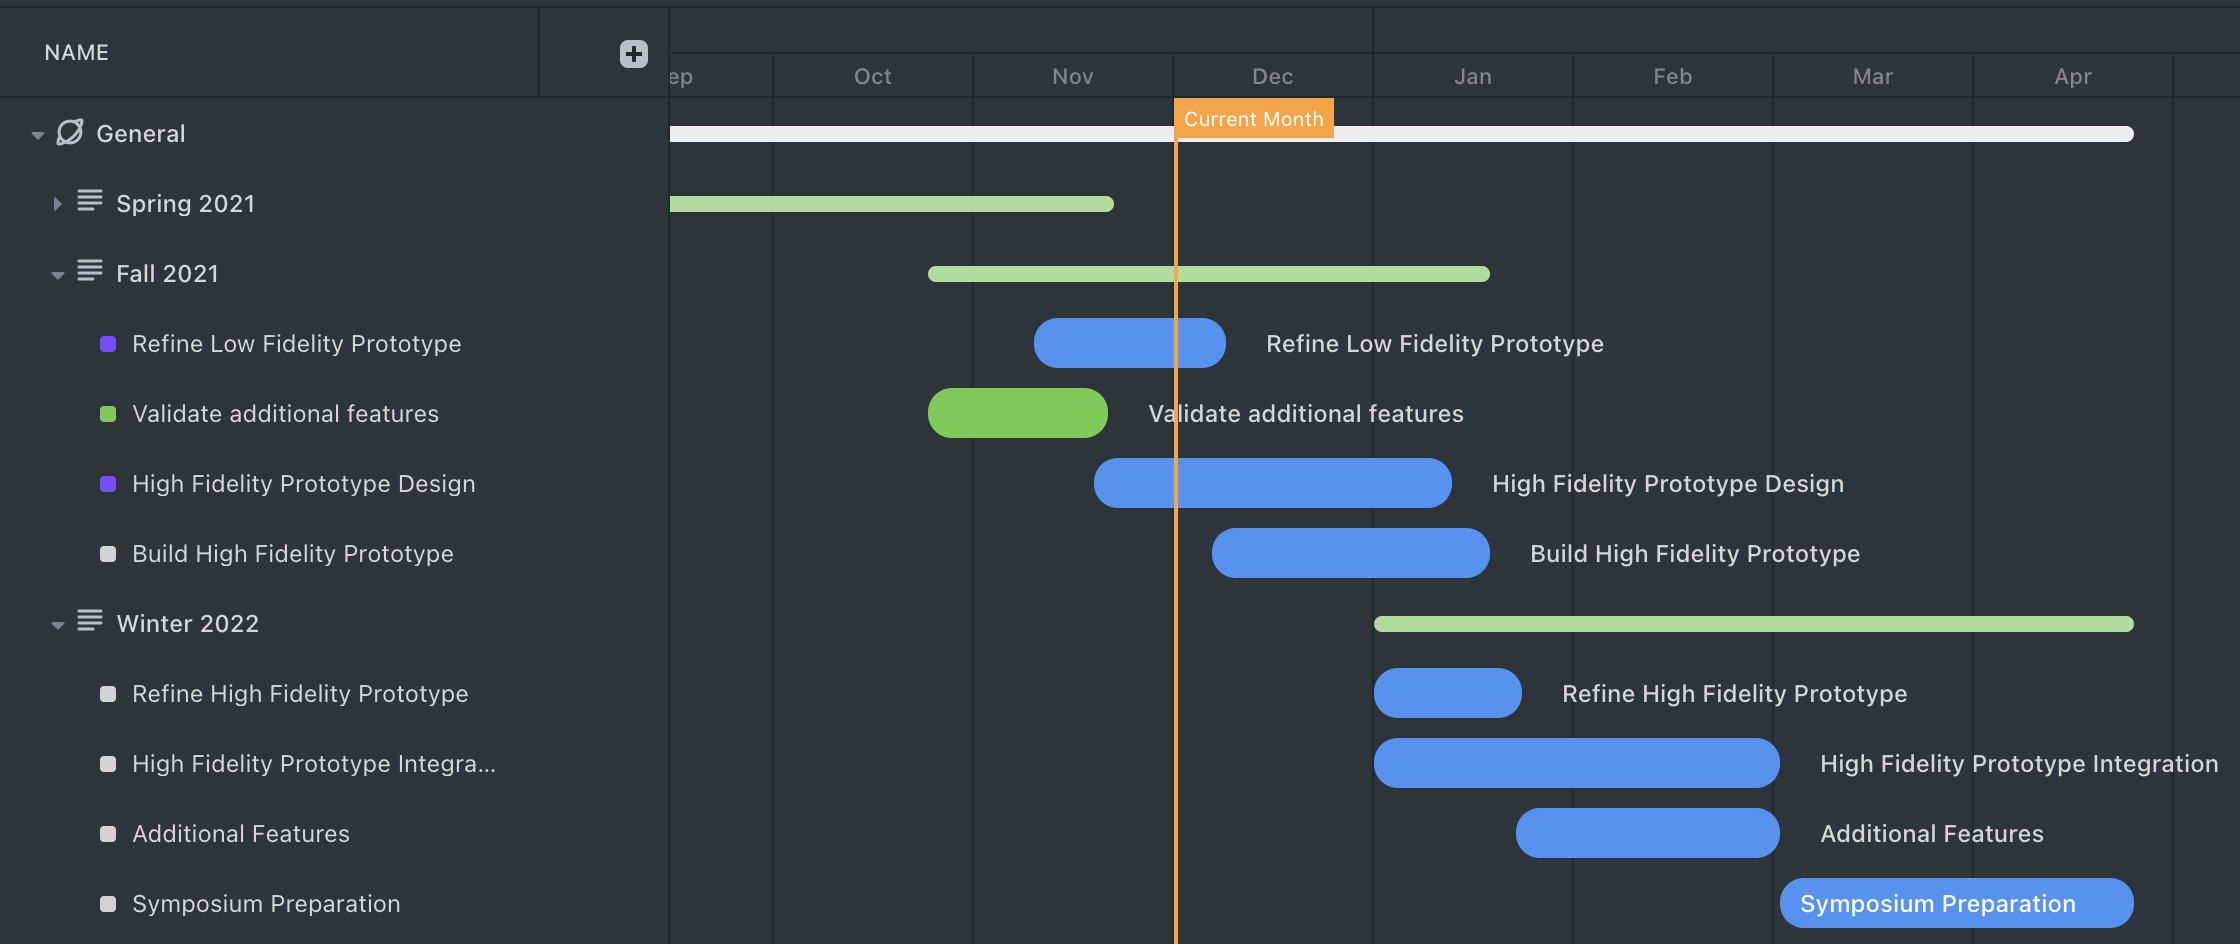
\includegraphics[width={1.0\linewidth}]{img/general-gantt.png}
    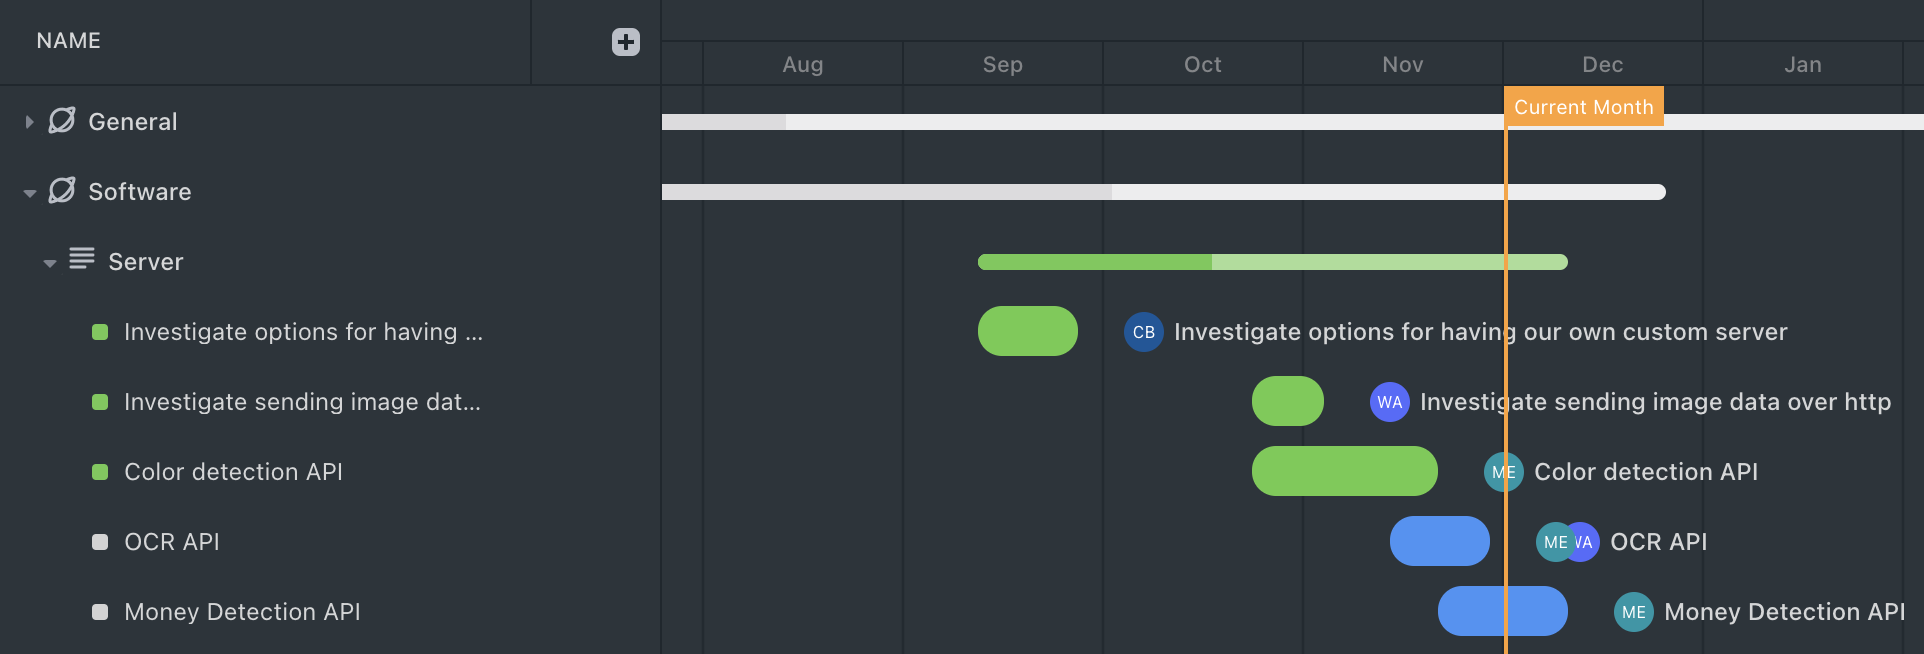
\includegraphics[width={1.0\linewidth}]{img/software-gantt-1.png}
    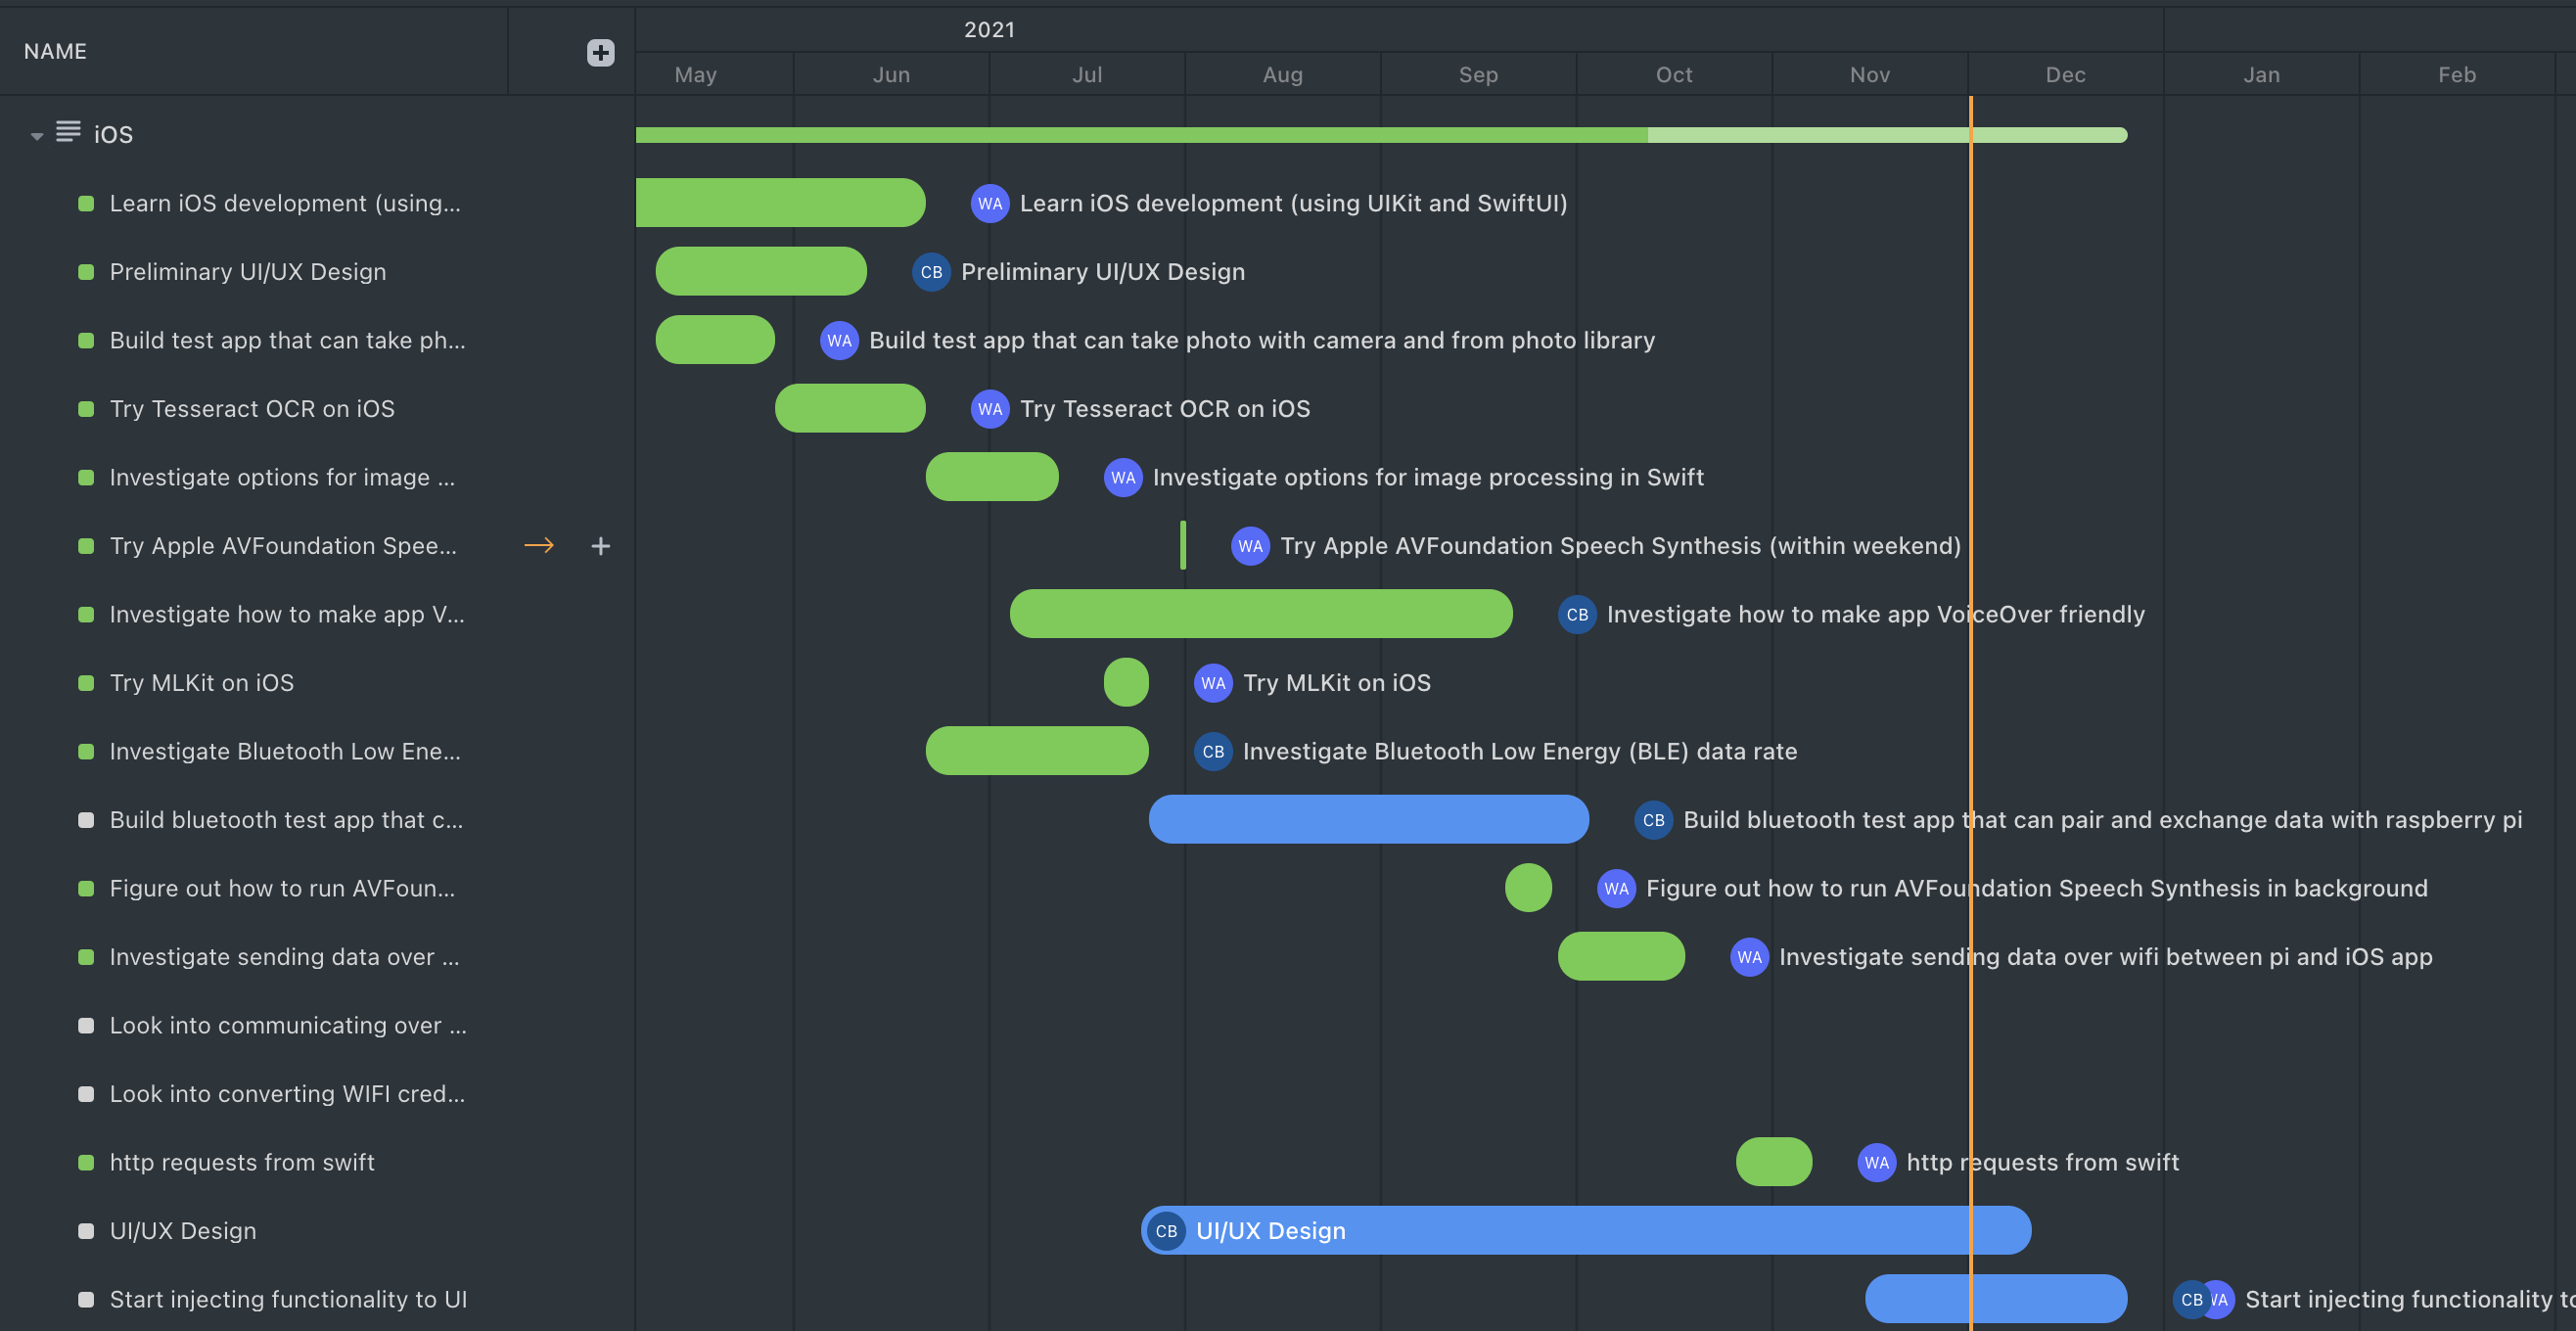
\includegraphics[width={1.0\linewidth}]{img/software-gantt-2.png}
    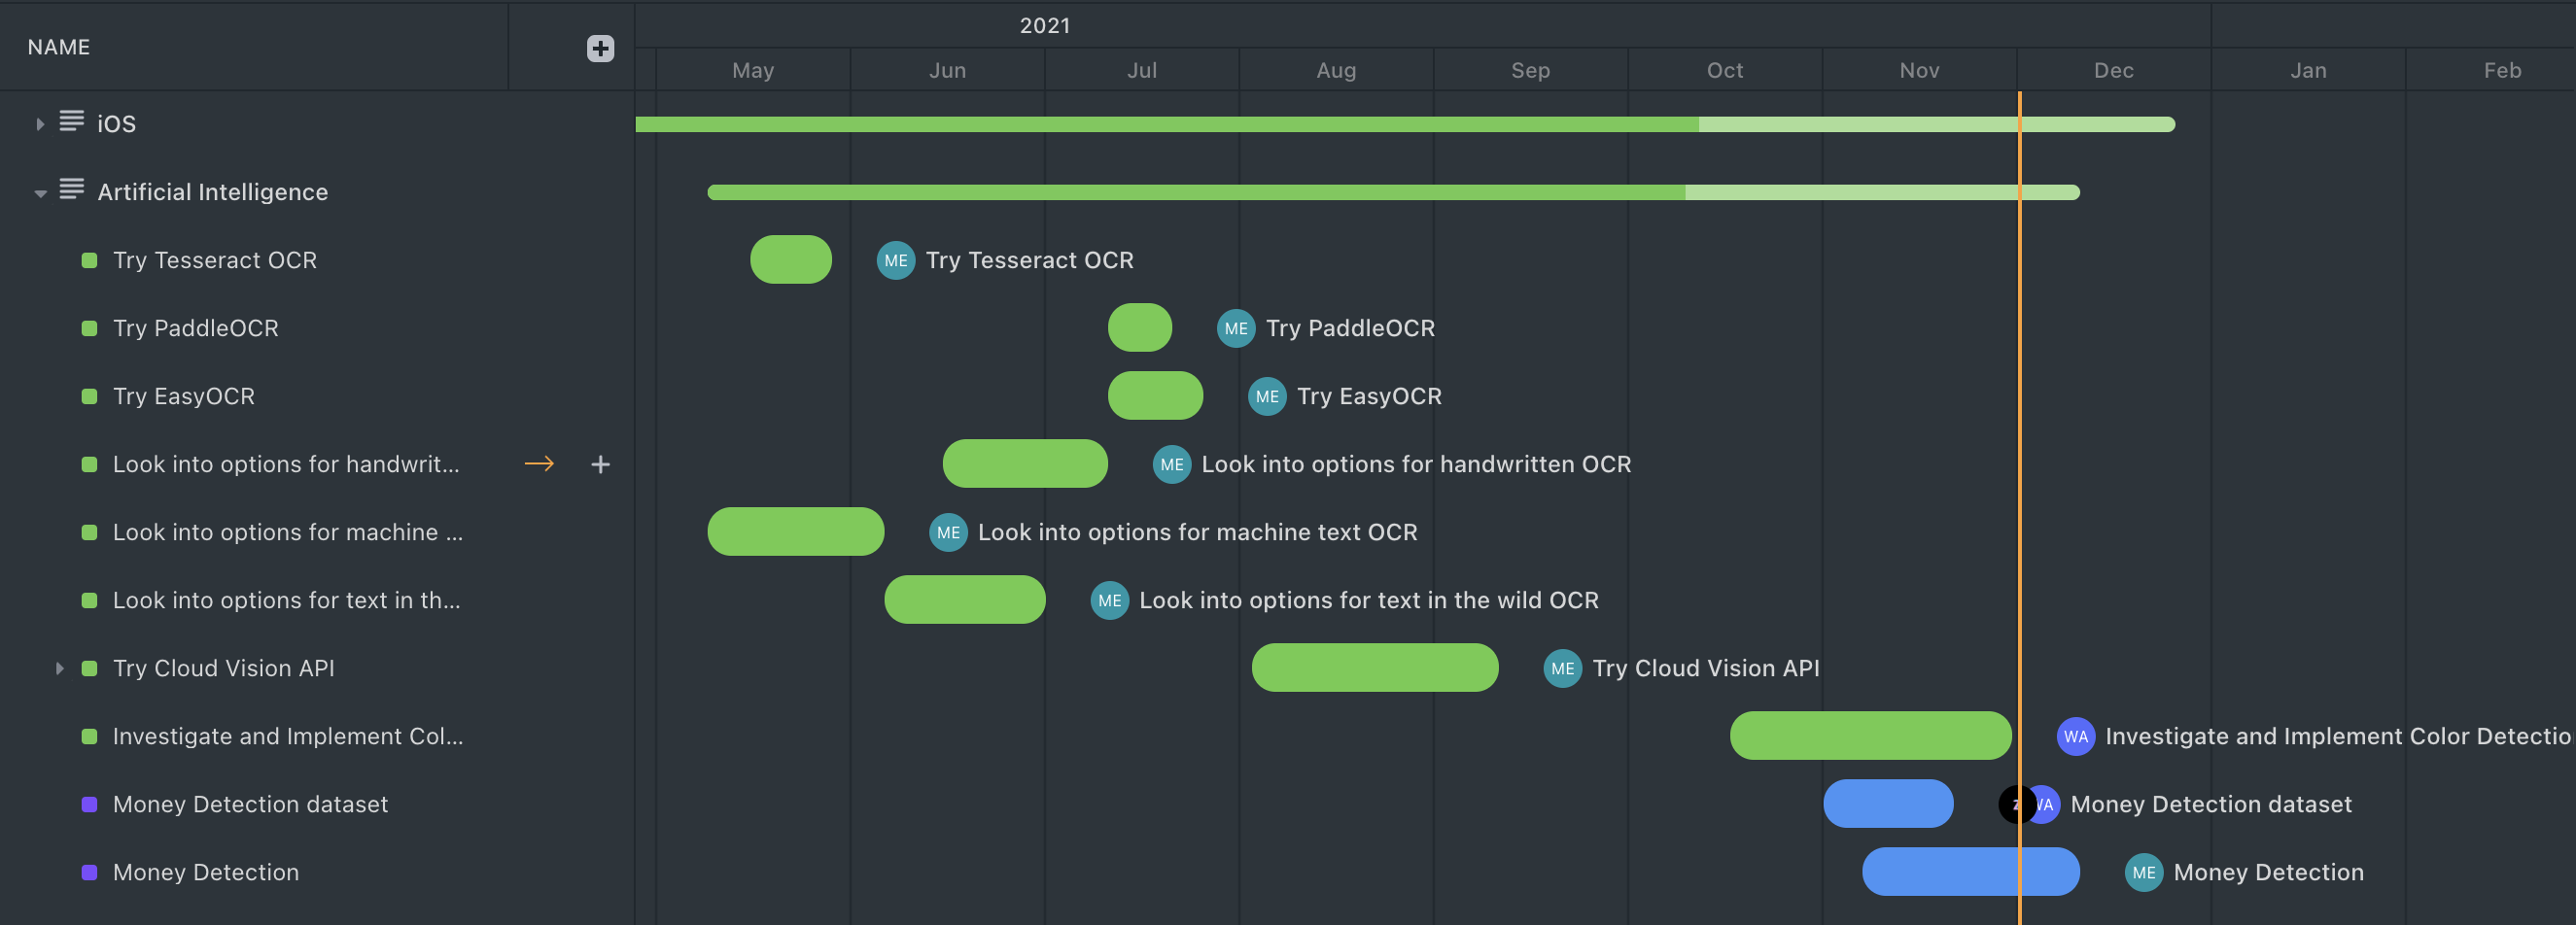
\includegraphics[width={1.0\linewidth}]{img/software-gantt-3.png}
    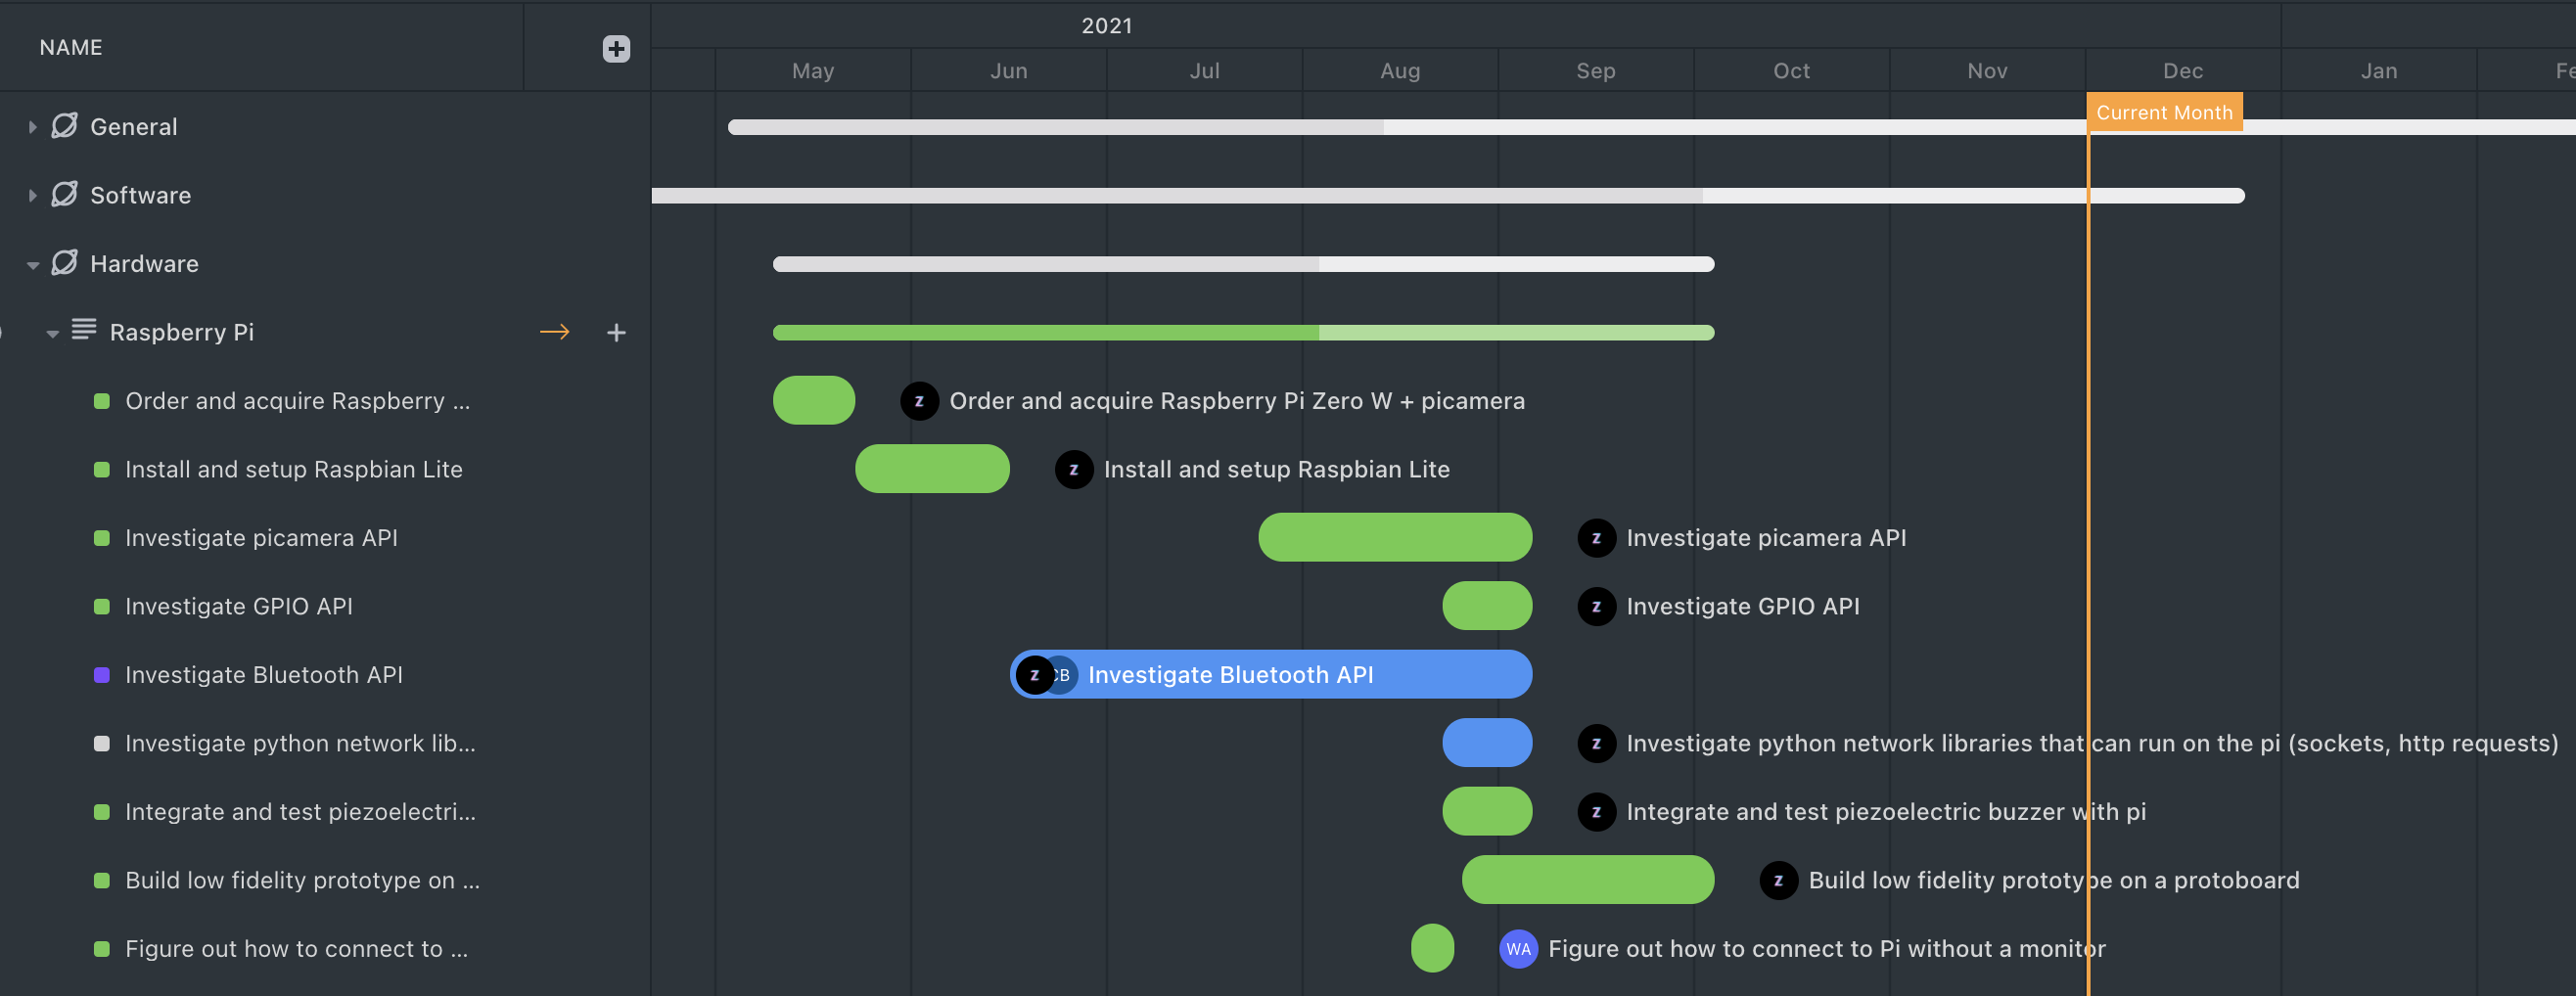
\includegraphics[width={1.0\linewidth}]{img/hardware-gantt.png}
\end{center}

\subsection{Budget}
The following table shows a breakdown of all materials and resources purchased and/or used during the term for the purpose of the project. The overall budget has not changed since the Spring 2021 term since no new parts have been added.

\begin{table}[ht]
    \centering
    \begin{tabular}{|l|c|r|}
        \hline
        
        \textbf{Item / Resource} & \textbf{Supplier} & \textbf{Cost (CAD)}
        \\ \hline
        Raspberry Pi Zero W Camera Pack & Adafruit      & 44.95
        \\ \hline
        SanDisk Ultra 32GB micro SDHC   & Amazon        & 12.79
        \\ \hline
        UGREEN Mini HDMI Adapter        & Amazon        & 10.99
        \\ \hline
        Electop USB Power Meter Tester  & Amazon        & 29.36
        \\ \hline
        Github Organization Free        & Github        & 0
        \\ \hline
        ClickUp Workspace               & ClickUP       & 0
        \\ \hline
        Overleaf Online LaTeX Editor    & Overleaf      & 0
        \\ \hline
        Labour Costs                    & N/A           & 15,120
        \\ \hline
        \textbf{Total}                  & \multicolumn{2}{r|}{\textbf{15218.09}}
        \\ \hline
    \end{tabular}
    \label{Tab:budget}
\end{table}
As a note, Labour costs were estimated using a rate (per student) of \$35/hour, 9 hour/week workload, and a 12-week term.

\subsection{Organizational Chart}
\begin{table}[ht]
    \centering
    % \begin{tabular}{|c|c|c|c|}
    \begin{tabular}{|p{2.8cm}|p{5.5cm}|p{6.5cm}|}
        \hline
        Name & Position & Responsibilities \\ \hline
        Waleed Ahmed & Project Manager & Driving discussions, scheduling, brainstorming, meeting logs, general support on prototyping and integration
        \\ \hline
        
        Martin Ethier & Artificial Intelligence Lead & 
        Research, testing, and integration of artificial intelligence software
        \\ \hline
        
        Zain Denno & Hardware and Embedded Lead & 
        Research, testing, and integration of the hardware platform \\ \hline
        
        Connor Barker & iOS Lead & 
        Research, testing, and integration of the mobile iOS application \\ \hline
        
        John Zelek & Faculty Advisor (SYDE) & Problem space and technical consultation \\ \hline
        
        Oscar Nespoli & GENE Course Instructor & Engineering design guidance through GENE 403 and 404 course content \\ \hline
    \end{tabular}
\end{table}

\newpage
\subsection{Risk Register}
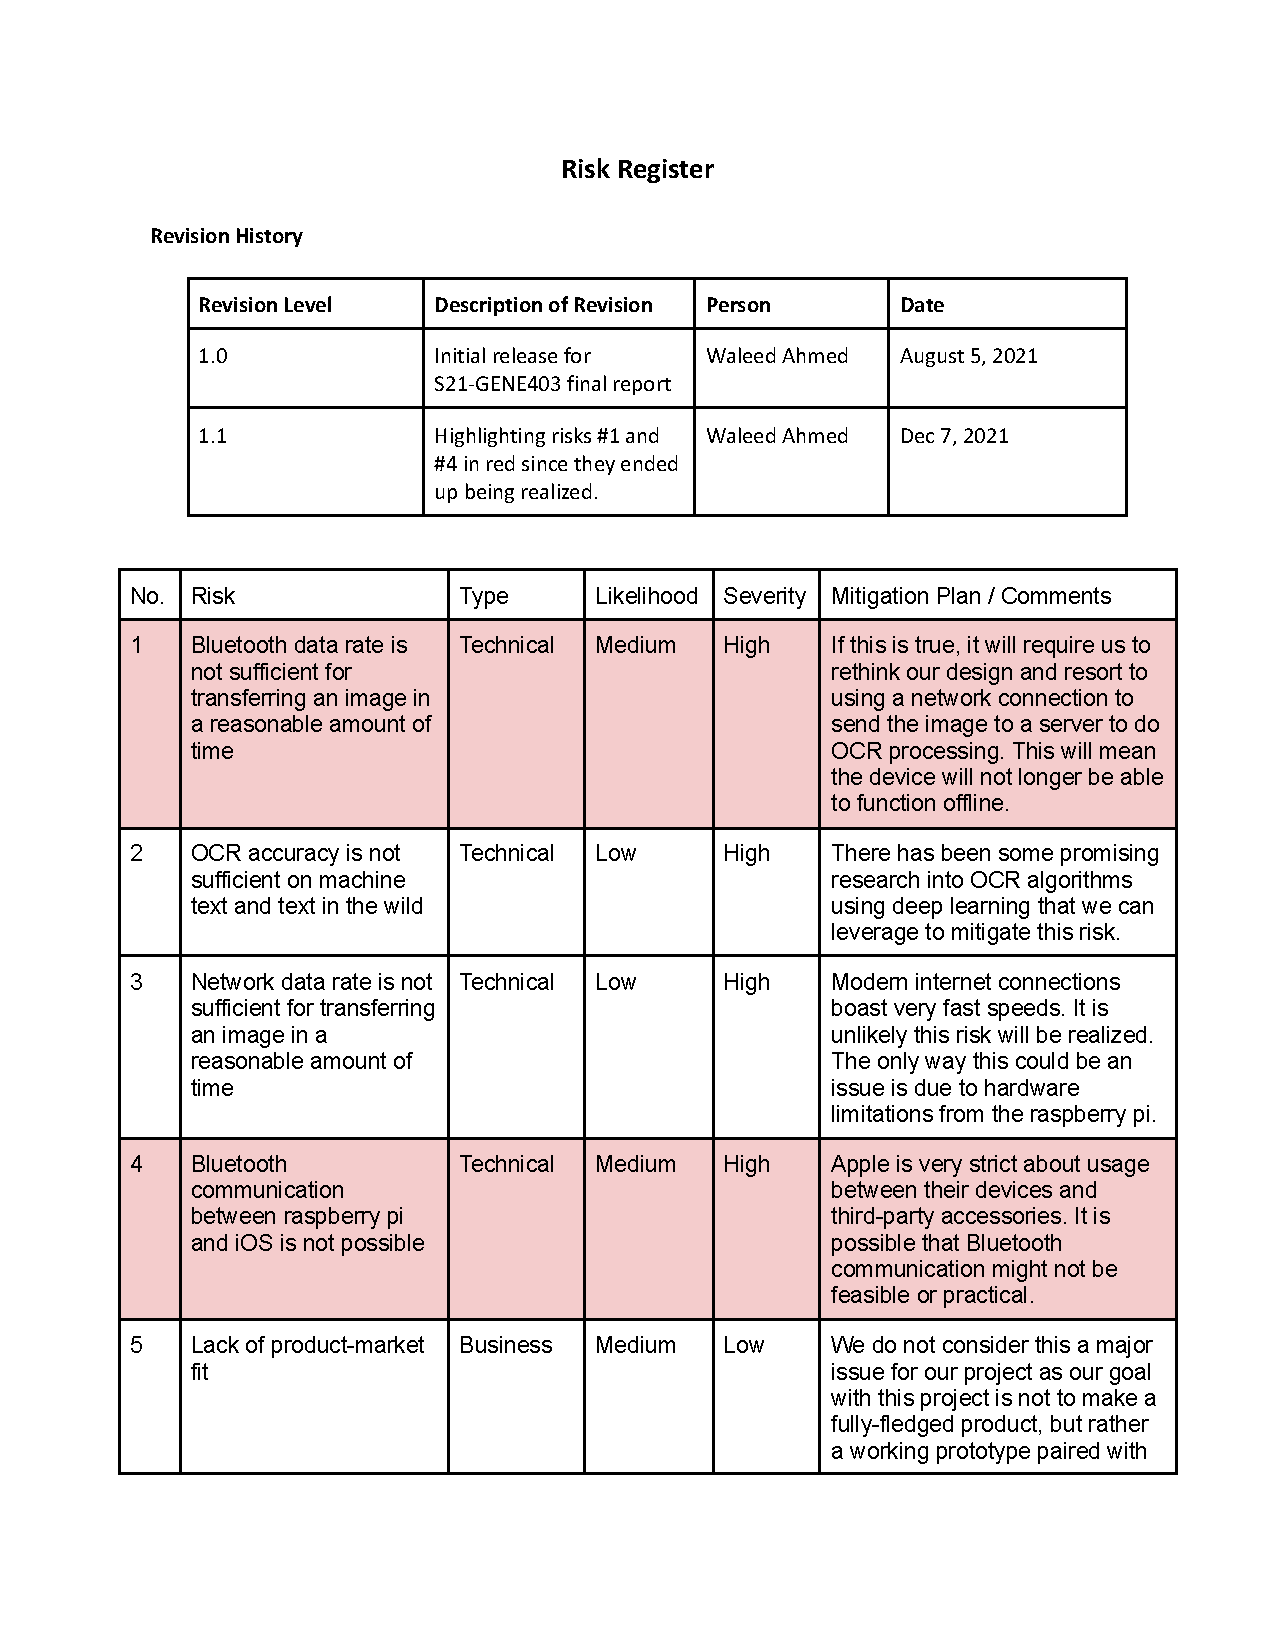
\includegraphics[page=1,width={1.0\linewidth}]{pdf/risk-register-1.1.pdf}
\newpage
\includegraphics[page=2,width={1.0\linewidth}]{pdf/risk-register-1.1.pdf}

\newpage
\subsection{Meeting Logs}
\label{meeting-logs}
Throughout the term, we used a shared Notion drive to hold all meeting logs and research notes.
Below are some screenshots that showcase the organization of the drive and the format we followed for keeping track of meeting logs.

\begin{center}
    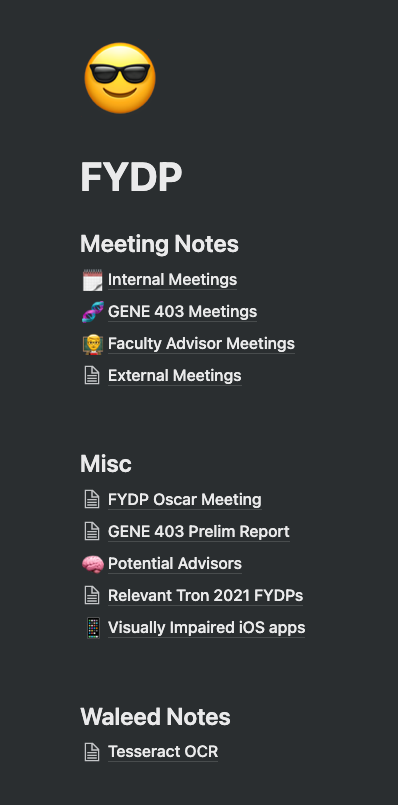
\includegraphics[width={0.3\linewidth}]{img/notion/notion1.png}
    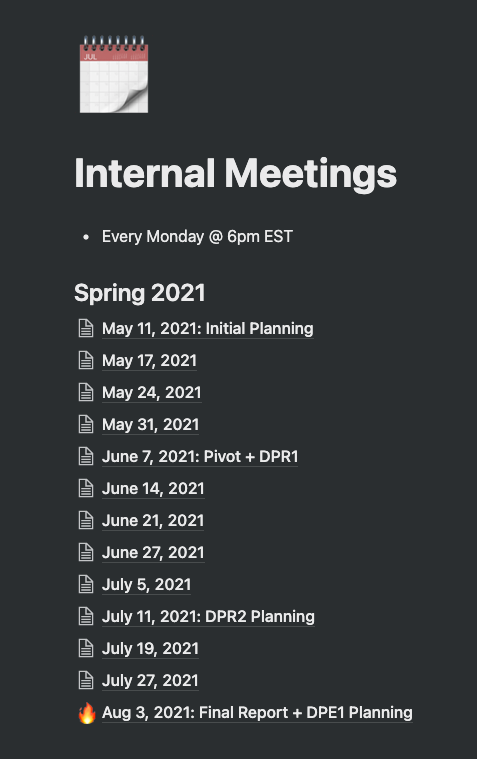
\includegraphics[width={0.35\linewidth}]{img/notion/notion2.png}
    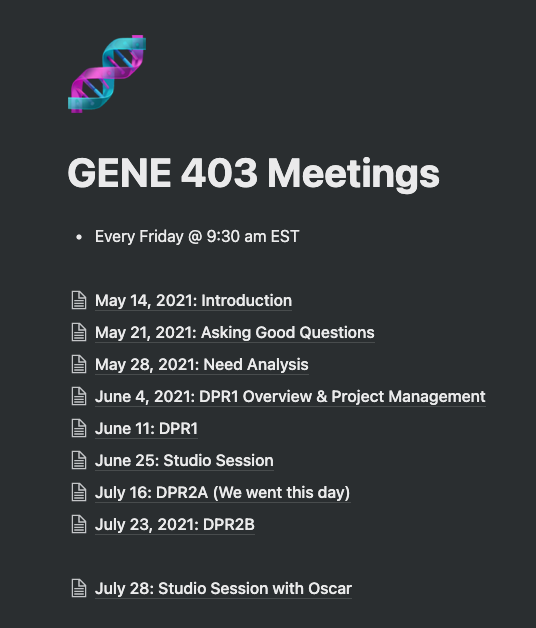
\includegraphics[width={0.3\linewidth}]{img/notion/notion3.png}
    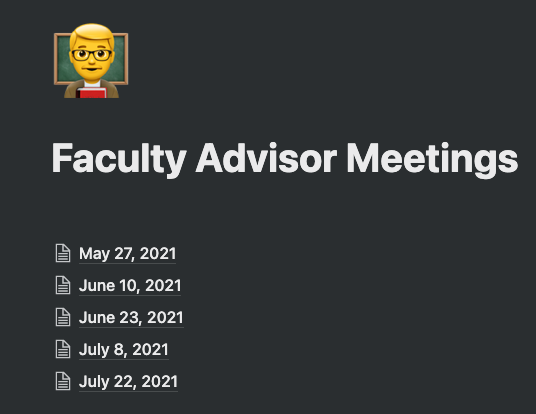
\includegraphics[width={0.3\linewidth}]{img/notion/notion4.png}
    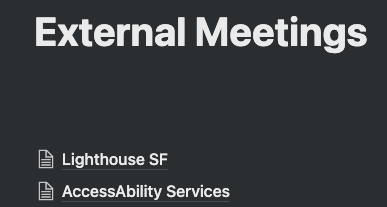
\includegraphics[width={0.3\linewidth}]{img/notion/notion5.png}
\end{center}

\newpage

For the internal meeting notes, the format we converged on naturally was:
\begin{itemize}
    \item Updates
        \begin{itemize}
            \item Waleed
            \item Connor
            \item Zain
            \item Martin
        \end{itemize}
    \item Discussion Topics
    \item Action Items
        \begin{itemize}
            \item Waleed
            \item Connor
            \item Zain
            \item Martin
        \end{itemize}
\end{itemize}

The idea is for each member to give updates on what they did the previous week, and then we go into any discussion items for that week, and finally end off with each member listing off their current action items. The expectation is that next week's updates will be based on the previous week's action items. An example of our notes from one of our meetings is shown below:
\begin{center}
    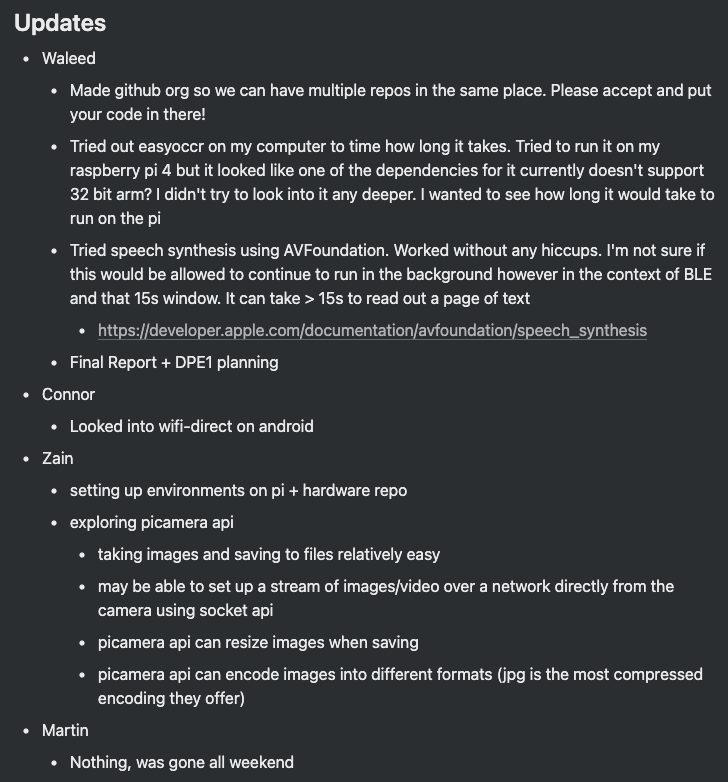
\includegraphics[width={0.5\linewidth}]{img/notion/Aug3_Updates.png} \\
    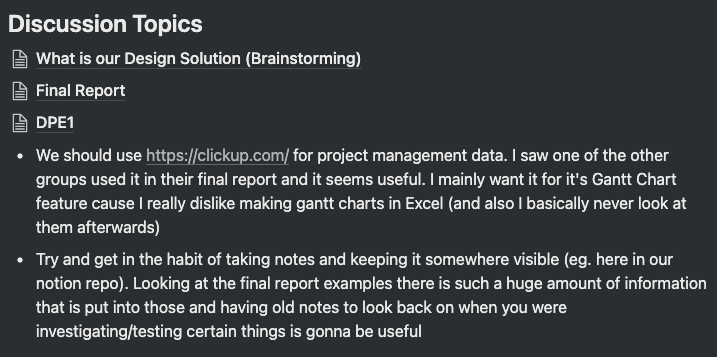
\includegraphics[width={0.45\linewidth}]{img/notion/Aug3_Discussion.png}
    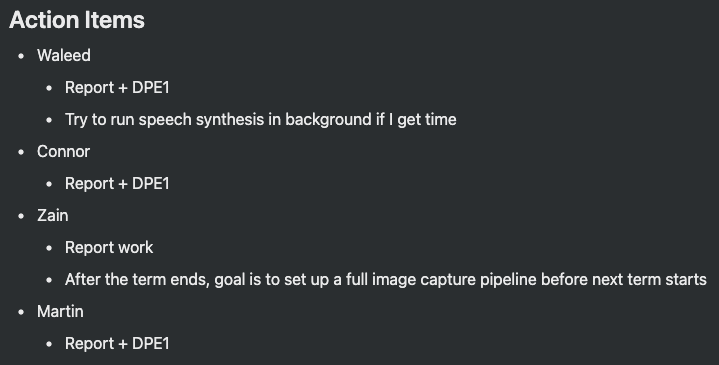
\includegraphics[width={0.45\linewidth}]{img/notion/Aug3_Action.png}
\end{center}

\section{Appendix D - Knowledge Application}
\label{appendix-D}

\subsection{OCR Testing Metrics}
Two metrics will be used to evaluate various OCR methods on our custom test sets. For machine text and handwritten text OCR, the word error rate metric is commonly used in the literature \cite{wer-metric}. For text-in-the-wild detection, the F-score metric is commonly used \cite{scene-text-rec}.

\subsubsection{Word Error Rate (WER)}
The Word Error Rate (WER) metric is very similar to the Character Error Rate (CER) metric. However, WER is typically a more useful metric if precise character-level accuracy is not required as long as the meaning of the sentence can be understood, which is the case for most OCR applications.

Both CER and WER are based on the concept of the Levenshtein Distance. In the context of CER, the Levenshtein Distance corresponds to the minimum number of single-character edits needed to transform one string into another. The allowed character edits are insertion, deletion, and substitution. To apply this to WER, the Levenshtein Distance can be adjusted to be the minimum number of word edits needed to transform a sequence of multiple words to another. \cite{wer-metric}

The following is an example for displaying the Levenshtein Distance between the words "visual" and "optical". The character edits needed to transform "visual" into "optical" can be seen below:
\begin{enumerate}
  \item \textbf{o}isual: substitute v with o at position 1
  \item o\textbf{p}isual: insert p at position 1
  \item op\textbf{t}isual: insert t at position 1
  \item opti\textbf{c}ual: substitute s with c at position 3
  \item opti\textbf{c}al: delete u at position 4
\end{enumerate}

Based on these edits, we can see the Levenshtein Distance is 5. In order to calculate the Levenshtein Distance between two strings, dynamic programming is used. This algorithm will also provide the number of insertions, deletions, and substitutions. These edit counts are what are used in the end to calculate the WER. The dynamic programming algorithm recursively splits the task into smaller tasks of finding the Levenshtein Distance on sub-strings. This generates a DP table. The DP table generated for the example above can be seen in Table \ref{tab:levenshtein_table}. The counts for substitutions, insertions, and deletions can be determined by looking at the number of diagonal, horizontal, and vertical transitions along the highlighted path in the DP table. The final Levenshtein Distance is the value in the bottom-right corner of the table. \cite{levenshtein-dist}

\begin{table}[H]
\begin{center}
\caption{Levenshtein DP table for transforming "visual" to "optical".}
\begin{tabular}{ c|c c c c c c c c } 
  &   & o & p & t & i & c & a & l \\ \hline
  & \textcolor{red}{0} & 1 & 2 & 3 & 4 & 5 & 6 & 7 \\
 v & 1 & \textcolor{red}{1} & \textcolor{red}{2} & \textcolor{red}{3} & 4 & 5 & 6 & 7 \\
 i & 2 & 2 & 2 & 3 & \textcolor{red}{3} & 4 & 5 & 6 \\
 s & 3 & 3 & 3 & 3 & 4 & \textcolor{red}{4} & 5 & 6 \\
 u & 4 & 4 & 4 & 4 & 4 & \textcolor{red}{5} & 5 & 6 \\
 a & 5 & 5 & 5 & 5 & 5 & 5 & \textcolor{red}{5} & 6 \\
 l & 6 & 6 & 6 & 6 & 6 & 6 & 6 & \textcolor{red}{5} \\
\end{tabular}
\label{tab:levenshtein_table}
\end{center}
\end{table}

These edit counts can then be fed into Equation \ref{eq:CER} for CER. Where S, D, and I are the number of substitutions, deletions, and insertions respectively and N is the total number of characters in the ground truth string. Note that for Equation \ref{eq:WER}, the counts correspond to full word edits and the denominator is the total number of words in the ground truth text. \cite{wer-metric}

\begin{equation}
\label{eq:CER}
CER=\frac{S+D+I}{N}
\end{equation}

\begin{equation}
\label{eq:WER}
WER=\frac{S_w+D_w+I_w}{N_w}
\end{equation}

\subsubsection{F-Score}
An OCR system typically consists of text detection followed by recognition. In the context of machine text, the difficulty of the detection is negligible. Therefore, a metric that evaluates recognition is only required. However, for text-in-the-wild OCR, the detection task is much more difficult. A metric that takes detection accuracy into account should be used. What is commonly used in research is the F-score metric.

To calculate the F-score for a given example, counts for true positives (TP), false positives (FP), and false negatives (FN) are needed. A TP in this case is defined as a bounding box prediction which firstly has an intersection over union (IoU) above a certain threshold with any ground truth bounding box and secondly predicts the correct text corresponding to the ground truth. The definition of IoU can be seen in Figure \ref{fig:iou-equation}.

\begin{figure}[H]
\centering
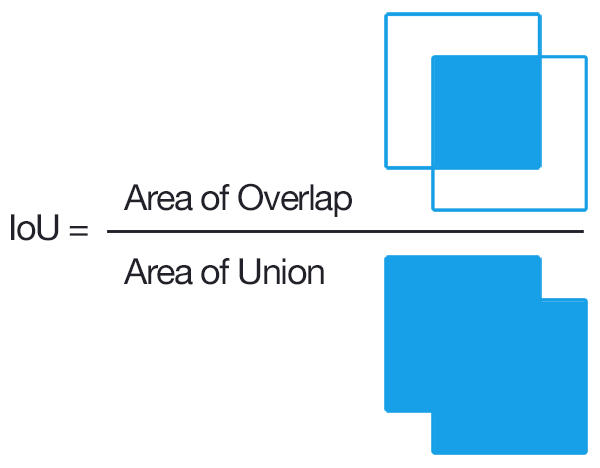
\includegraphics[scale=0.5]{img/iou_equation.png}
\caption{Description of the Intersection over Union (IoU) metric. \cite{iou-object-detection}}
\label{fig:iou-equation}
\end{figure}

False positives are then defined as bounding box predictions that do not have an IoU above the desired threshold with any ground truth bounding box or pass the desired IoU but do not provide the correct text prediction. False negatives are defined as any ground truth bounding boxes that do not have any predictions corresponding as true positives with them. As seen in Equations \ref{eq:precision}, \ref{eq:recall}, and \ref{eq:f-score}, these values can then be used to calculate precision (P) and recall (R), which can then be used to calculate the F-score (F) value.

\begin{equation}
\label{eq:precision}
P=\frac{TP}{TP+FP}
\end{equation}

\begin{equation}
\label{eq:recall}
R=\frac{TP}{TP+FN}
\end{equation}

\begin{equation}
\label{eq:f-score}
F=2*\frac{P*R}{P+R}
\end{equation}

\newpage
% REFERENCES
\begin{thebibliography}{9}
\bibitem{orbis-global-blind-data}
“Number of blind people set to triple by 2050” Orbis, 09-Feb-2021. [Online]. Available: https://can.orbis.org/en/news/2017/number-of-blind-people-set-to-triple-by-2050-1. [Accessed: 02-Aug-2021]. 

\bibitem{cnib-blind-data}
“Blindness in Canada” CNIB. [Online]. Available: https://cnib.ca/en/sight-loss-info/blindness/blindness-canada?region=on. [Accessed: 02-Aug-2021]. 

\bibitem{nfb-blind-data}
“Blindness Statistics” NFB, Jan-2019. [Online]. Available: https://nfb.org/resources/blindness-statistics. [Accessed: 02-Aug-2021]. 

\bibitem{lighthouse-sf-info-page}
“What does ‘blind’ really mean?” LightHouse for the Blind and Visually Impaired, 28-Jan-2019. [Online]. Available: https://lighthouse-sf.org/about/getting-started/. [Accessed: 02-Aug-2021]. 

\bibitem{WHO-blindness}
“Vision impairment and blindness” World Health Organization. [Online]. Available: https://www.who.int/news-room/fact-sheets/detail/blindness-and-visual-impairment. [Accessed: 02-Aug-2021]. 

\bibitem{lighthouse-sf-homepage}
LightHouse for the Blind and Visually Impaired, 22-Aug-2019. [Online]. Available: https://lighthouse-sf.org/. [Accessed: 02-Aug-2021].

\bibitem{uw-accessability}
AccessAbility Services, 08-Jul-2021. [Online]. Available: https://uwaterloo.ca/accessability-services/. [Accessed: 03-Aug-2021]. 

\bibitem{jaws-software}
“Jaws®” Freedom Scientific. [Online]. Available: https://www.freedomscientific.com/products/
software/jaws/. [Accessed: 03-Aug-2021].

\bibitem{kurzweil}
K. Education, Assistive learning technologies \& literacy software from KURZWEIL Education. [Online]. Available: https://www.kurzweiledu.com/default.html. [Accessed: 03-Aug-2021]. 

\bibitem{read-and-write}
“Read \& write for education - reading, literacy \& assistive software” Texthelp. [Online]. Available: https://www.texthelp.com/en-gb/products/read-and-write-education/. [Accessed: 03-Aug-2021]. 

\bibitem{speechify}
Speechify. [Online]. Available: https://speechify.com/. [Accessed: 03-Aug-2021]. 

\bibitem{clickup}
“ClickUp™ | one app to replace them all.” [Online]. Available: https://clickup.com/. [Accessed: 07-Aug-2021]. 

\bibitem{orcam}
OrCam MyEye 2.0. [Online]. Available: https://www.orcam.com/en/myeye2/. [Accessed: 08-Aug-2021].

\bibitem{orcam-price}
B. Holton, “MyReader and MyEye from OrCam: Text and item recognition at the touch of a finger,” The American Foundation for the Blind. [Online]. Available: https://www.afb.org/aw/18/2/15244. [Accessed: 08-Aug-2021]. 

\bibitem{orcam-amazon}
“OrCam MyEye Pro ,” Amazon.ca: Electronics. [Online]. Available: https://www.amazon.ca/OrCam-Inc-MyEye-2/dp/B07H31SBMW. [Accessed: 08-Aug-2021].

\bibitem{WHO-assistive}
“Assistive technology,” World Health Organization. [Online]. Available: https://www.who.int/news-room/fact-sheets/detail/assistive-technology. [Accessed: 08-Aug-2021]. 

\bibitem{envision}
Envision. [Online]. Available: https://www.letsenvision.com/. [Accessed: 08-Aug-2021].

\bibitem{seeing-ai}
Seeing AI App from Microsoft. [Online]. Available: https://www.microsoft.com/en-us/ai/seeing-ai. [Accessed: 08-Aug-2021]. 

\bibitem{speechify}
Speechify. [Online]. Available: https://speechify.com/. [Accessed: 08-Aug-2021]. 

\bibitem{be-my-eyes}
Be My Eyes - See the world together. [Online]. Available: https://www.bemyeyes.com/. [Accessed: 08-Aug-2021]. 

\bibitem{tesseract-github}
“Tesseract-Ocr/Tesseract: Tesseract open source ocr engine (main repository),” GitHub. [Online]. Available: https://github.com/tesseract-ocr/tesseract. [Accessed: 09-Aug-2021]. 

\bibitem{apple-speech-synthesis}
“Speech Synthesis,” Apple Developer Documentation. [Online]. Available: https://developer.apple.com/documentation/avfoundation/speech\_synthesis. [Accessed: 09-Aug-2021]. 

\bibitem{tesseract-improve-quality}
“Improving the quality of the output,” tessdoc. [Online]. Available: https://tesseract-ocr.github.io/tessdoc/ImproveQuality.html. [Accessed: 09-Aug-2021]. 

\bibitem{apple-mfi}
“Create innovative Accessories,” MFi Program. [Online]. Available: https://mfi.apple.com/. [Accessed: 10-Aug-2021]. 

\bibitem{apple-wac}
“Wireless Accessory Configuration Entitlement,” Apple Developer Documentation. [Online]. Available: https://developer.apple.com/documentation/bundleresources/entitlements/com\_apple\_external-accessory\_wireless-configuration. [Accessed: 10-Aug-2021]. 

\bibitem{rpi-zero-w}
“Raspberry Pi Zero W,” Raspberry Pi. [Online]. Available: https://www.raspberrypi.org/products/raspberry-pi-zero-w/. [Accessed: 10-Aug-2021]. 

\bibitem{rpi-camera}
“Camera Module 2,” Raspberry Pi. [Online]. Available: https://www.raspberrypi.org/products/camera-module-v2/. [Accessed: 10-Aug-2021]. 

\bibitem{wer-metric}
K. Leung, “Evaluate ocr output quality with character error rate (cer) and word error rate (wer),” Medium, 27-Jul-2021. [Online]. Available: https://towardsdatascience.com/evaluating-ocr-output-quality-with-character-error-rate-cer-and-word-error-rate-wer-853175297510. [Accessed: 10-Aug-2021].

\bibitem{levenshtein-dist}
“Levenshtein distance,” Wikipedia, 09-Mar-2021. [Online]. Available: https://en.wikipedia.org/wiki/Levenshtein\_distance. [Accessed: 10-Aug-2021].

\bibitem{scene-text-rec}
Y. Cao, S. Ma, and H. Pan, “FDTA: Fully CONVOLUTIONAL Scene text detection with TEXT ATTENTION,” IEEE Access, vol. 8, pp. 155441–155449, 2020.

\bibitem{iou-object-detection}
A. Rosebrock, “Intersection over Union (iou) for object detection,” PyImageSearch, 01-Jul-2021. [Online]. Available: https://www.pyimagesearch.com/2016/11/07/intersection-over-union-iou-for-object-detection. [Accessed: 10-Aug-2021].

\bibitem{paddle-ocr}
PaddlePaddle, “PaddlePaddle/PaddleOCR: Awesome Multilingual OCR toolkits based on PaddlePaddle (practical ultra lightweight OCR system, support 80+ Languages recognition, provide data annotation and synthesis tools, support training and deployment among server, mobile, embedded and Iot devices),” GitHub. [Online]. Available: https://github.com/PaddlePaddle/PaddleOCR. [Accessed: 10-Aug-2021].

\bibitem{easy-ocr}
JaidedAI, “JaidedAI/EasyOCR: Ready-to-use OCR with 80+ supported languages and all popular writing scripts including Latin, Chinese, Arabic, Devanagari, Cyrillic and etc.,” GitHub. [Online]. Available: https://github.com/JaidedAI/EasyOCR. [Accessed: 10-Aug-2021].

\bibitem{orcam-patents}
https://www.orcam.com/en/patents/

\bibitem{envision-patent}
https://patents.google.com/patent/US9805619B2/en

\bibitem{orcam-hardware}
https://patents.google.com/patent/US8902303B2/en

\bibitem{orcam-software}
https://patents.justia.com/patent/9911361

\bibitem{doctrine-of-equivalents}
“Doctrine of Equivalents”, Wikipedia, 02-Jun-2021. [Online]. Available: https://en.wikipedia.org/wiki/Doctrine\_of\_equivalents. [Accessed: 09-Aug-2021].

\bibitem{pipeda}
https://www.priv.gc.ca/en/privacy-topics/privacy-laws-in-canada/the-personal-information-protection-and-electronic-documents-act-pipeda/pipeda\_brief/

\bibitem{ewaste}
"What Are The Right Electronic Waste Disposal Methods?", Dawn DeVroom, 30-Apr-2019. [Online]. Available: https://blog.idrenvironmental.com/what-are-the-right-electronic-waste-disposal-methods. [Accessed: 9-Aug-2021]

\bibitem{neural-efficiency}
“Apple A11”, Wikipedia, 02-Jun-2021. [Online]. Available:
https://en.wikipedia.org/wiki/Apple\_A11. [Accessed: 9-Aug-2021].

\bibitem{iphone-recycle}
https://www.apple.com/ca/environment/

\bibitem{apple-bluetooth}
“Core Bluetooth”, Apple Developer Documentation. [Online]. Available: https://developer.apple.com/documentation/corebluetooth. [Accessed: 09-Aug-2021]. 

\bibitem{raspi-hardware}
https://www.raspberrypi.org/products/raspberry-pi-zero-w/

\bibitem{iphone-hardware}
“iPhone X Specifications”, Apple. [Online]. Available: https://support.apple.com/kb/sp770?locale=en\_CA. [Accessed: 09-Aug-2021]. 

\bibitem{bluetooth-classic}
"Bluetooth Classic vs Bluetooth Low Energy (BLE) on Android", D. Kliszowki, A. Vlasov. [Online]. Available: https://www.thedroidsonroids.com/blog/bluetooth-classic-vs-bluetooth-low-energy-ble. [Accessed: 09-Aug-2021].

\bibitem{resnet}
Singhal, G. (2020, May 5). Gaurav Singhal. Pluralsight. Retrieved December 4, 2021, from https://www.pluralsight.com/guides/introduction-to-resnet.


\end{thebibliography}

\end{document}
